\documentclass[11pt, openany]{article}
%\usepackage{pstricks,pstricks-add,pst-math,pst-xkey}
\usepackage[frenchb]{babel}
%\usepackage{slashbox}
\usepackage{graphicx}
\usepackage{amsmath,amssymb,amstext}
\usepackage[latin1]{inputenc}
\usepackage[OT1]{fontenc}
%\usepackage{fancybox}
\usepackage{a4wide}
%\usepackage{fancyvrb}
\usepackage{pgf,tikz} %arbres
%\usetikzlibrary{arrows}
\usepackage{xcolor}
%\usepackage{multicol}
%\usepackage[cm]{fullpage}
\usepackage{amsthm} %pour les th�or�mes sans num�ro
\usepackage{array,multirow,makecell}
\usepackage{mathrsfs}

\usepackage{floatflt}

\usepackage{bussproofs}\EnableBpAbbreviations


\bibliographystyle{ieeetr}  


\newcounter{moncompteur}
\newtheorem{q}[moncompteur]{\textbf{Question}}{}
\newtheorem{prop}[moncompteur]{\textbf{Proposition}}{}
\newtheorem{df}[moncompteur]{\textbf{D�finition}}{}
\newtheorem*{df*}{\textbf{D�finition}}{}
\newtheorem{rem}[moncompteur]{\textbf{Remarque}}{}
\newtheorem{theo}[moncompteur]{\textbf{Th�or�me}}{}
\newtheorem*{theo*}{\textbf{Th�or�me}}{}
\newtheorem{conj}[moncompteur]{\textbf{Conjecture}}{}
\newtheorem{cor}[moncompteur]{\textbf{Corollaire}}{}
\newtheorem{lm}[moncompteur]{\textbf{Lemme}}{}
\newtheorem*{lm*}{\textbf{Lemme}}{}
%\newtheorem{nota}[moncompteur]{ \textbf{Notation}}{}
%\newtheorem{conv}[moncompteur]{ \textbf{Convention}}{}
\newtheorem{exa}[moncompteur]{\textbf{Exemple}}{}
\newtheorem{ex}[moncompteur]{\textbf{Exercice}}{}
%\newtheorem{app}[moncompteur]{ \textbf{Application}}{}
%\newtheorem{prog}[moncompteur]{ \textbf{Algorithme}}{}
%\newtheorem{hyp}[moncompteur]{ \textbf{Hypoth�se}}{}
%\newenvironment{dem}{\noindent\textbf{Preuve}\\}{\flushright$\blacksquare$\\}
%\newenvironment{dem}{\noindent\textbf{Preuve.} }{\hfill$\blacksquare$\\}

%\newenvironment{myindentpar}[1]%
%{\begin{list}{}%
%         {\setlength{\leftmargin}{#1}}%
%         \item[]%
%}
%{\end{list}}



%\newcommand{\R}{\mathbb{R}}
%\newcommand{\K}{\mathbb{K}}
%\newcommand{\N}{\mathbb{N}}
%\newcommand{\Z}{\mathbb{Z}}
%\newcommand{\C}{\mathbb{C}}
%\newcommand{\U}{\mathbb{U}}
%\newcommand{\Q}{\mathbb{Q}}
%\newcommand{\card}{\mathrm{card}}


\newcommand{\s}{\sigma}
%\newcommand{\l}{\lambda}
%\newcommand{\a}{\alpha}
%\newcommand{\r}{\rho}

%m�moire
\newcommand{\Ccal}{\mathcal{C}}
\newcommand{\Dcal}{\mathcal{D}}
\newcommand{\1}{\boldsymbol{1}}
\newcommand{\CProofs}{
%?\mathcal{C}?
\mathcal{CP}
}
%

\newcommand{\subsectionDescription}[1]{
\addtocontents{toc}{%\textit{
%\qquad\qquad
\hangindent=3.5\parindent \hangafter=0
\noindent
#1
}%}
}


\newcommand{\idees}[1]{
\textsf{(#1)}
}



%stage
\newcommand{\LK}{$\mathbf{LK}$}
\newcommand{\LJ}{$\mathbf{LJ}$}
\newcommand{\LJT}{$\mathbf{LJT}$}
\newcommand{\LSJ}{$\mathbf{LSJ}$}
\newcommand{\LSJn}{$\mathbf{LSJ\boldsymbol\ell}$}


\newcommand{\Sig}{\mathfrak S}
\newcommand{\G}{\Gamma}
\newcommand{\D}{\Delta}
\newcommand{\Th}{\Theta}
\newcommand{\Gp}{\Gamma}
\newcommand{\Dp}{\Delta}
\newcommand{\Gt}{\widetilde\Gamma}
\newcommand{\Dt}{\widetilde\Delta}

\newcommand{\imp}{\to\negthickspace}

\newcommand{\surj}{
%\mathrm{surj}
\boldsymbol
\Phi
}
\newcommand{\To}{\Rightarrow}
\newcommand{\forget}{\mathsf{forget}}



\newcommand{\autour}[5]{
^{#2}_{#3}#1^{#4}_{#5}
}

\begin{document}
\renewcommand{\labelitemi}{$\bullet$}



%\begin{titlepage}
%\begin{center}
% {\huge\bfseries M�moire et rapport de stage \\---\\ Automates cellulaires \\ et probl�mes inverses : \\classification de la densit�\\--- \\�tude de la multiplication binaire et approches dynamiques pour la factorisation de nombres\\ }
% % ----------------------------------------------------------------
% \vspace{5cm}
% {\Large\bfseries Rapha�l Rieu-Helft}\\[5pt]
%% email@gmail.com\\[14pt]
%%   % ----------------------------------------------------------------
% \vspace{5cm}
%% {Thesis  submitted to} \\[5pt]
%% \emph{{Your University}}\\[2cm]
%% {in partial fulfilment for the award of the degree
%%  of} \\[2cm]
%% \textsc{\Large{{Doctor of Philosophy}}} \\[5pt]
%% {in some subject} \vspace{0.4cm} \\[2cm]
%% % {By}\\[5pt] {\Large \sc {Me}}
%%  \vfill
%%  % ----------------------------------------------------------------
%%\includegraphics[width=0.19\textwidth]{example-image-a}\\[5pt]
%{\Large M�moire encadr� par Jean Mairesse (LIAFA)}\\[5pt]
%\vspace{1.5em}
%{\Large Stage effectu� au LORIA sous la direction de Sylvain Contassot-Vivier (�quipe Algorille) et de Nazim Fat�s (�quipe Maia)}\\[5pt]
%
% \vfill
%{\Large �t� 2014}
%\end{center}
%\end{titlepage}

\begin{titlepage}
\begin{center}
\vspace*{3cm}
 {\huge\bfseries Calcul des s�quents et\\ transfert vers une cat�gorie\\}
  \vspace{.5cm}
 {\Large M�moire encadr� par Paul-Andr� Melli�s (PPS)\\}
 % ----------------------------------------------------------------
 \vspace{4cm}
  {\huge\bfseries Recherche de preuves compil�e et certifi�e\\}
  \vspace{.5cm}
 {\Large Stage effectu� au LORIA de Nancy\\
 au sein de l'�quipe TYPES\\
 sous la direction de Didier Galmiche et Dominique Larchey-Wendling\\}
 
  \vspace{5cm}
 
 {\Large\bfseries Diane Gallois-Wong}\\[5pt]
 \vspace{.7cm}
{\Large L3 \quad---\quad 2014}
\end{center}
\end{titlepage}




%regles et instances
\def\regle{
\def\defaultHypSeparation{\hskip .05in}
	\AXC	{$prem_{1}$}
	\AXC	{...}
	\AXC	{$prem_{p}$}
	\RightLabel{$(\mathcal R)$}
	\TIC{$concl$}
	\DP
}
\def\instance{
\def\defaultHypSeparation{\hskip .05in}
	\AXC	{$\s_{1}$}
	\AXC	{...}
	\AXC	{$\s_{p}$}
	\RightLabel{$(\mathcal R)$}
	\TIC{$\s$}
	\DP
}
\def\instanceAx{
\centerAlignProof
	\AXC	{\qquad}
	\RightLabel{$(\mathcal A)$}
	\UIC{$\s$}
	\DP
}
\def\instancedeux{
\def\defaultHypSeparation{\hskip .05in}
	\AXC	{$\s_{1}$}
	\AXC	{$\s_{2}$}
	\BIC{$\s$}
	\DP
}


%LJ
%LJ, axiomes
\def\LJid{
	\AXC	{}
	\RightLabel{$(id)$}
	\UIC{$A,\G \To A$}
	\DP
}
\def\LJbotL{
	\AXC	{}
	\RightLabel{$(\bot L)$}
	\UIC{$\bot,\G \To D$}
	\DP
}
%LJ,r�gles logiques
\def\LJetL{
	\AXC	{$A,B,\G \To D$}
	\RightLabel{$(\land L)$}
	\UIC{$A\land B,\G \To D$}
	\DP
}
\def\LJetR{
	\AXC	{$\G \To A$}
	\AXC	{$\G \To B$}
	\RightLabel{$(\land R)$}
	\BIC{$\G \To A\land B$}
	\DP
}
\def\LJouL{
	\AXC	{$A,\G \To D$}
	\AXC	{$B,\G \To D$}
	\RightLabel{$(\lor L)$}
	\BIC{$A\lor B,\G \To D$}
	\DP
}
\def\LJouRun{
	\AXC	{$\G \To A$}
	\RightLabel{$(\lor R_{1})$}
	\UIC{$\G \To A\lor B$}
	\DP
}
\def\LJouRdeux{
	\AXC	{$\G \To B$}
	\RightLabel{$(\lor R_{2})$}
	\UIC{$\G \To A\lor B$}
	\DP
}
\def\LJimpL{
	\AXC	{$\G \To A$}
	\AXC	{$B,\G \To D$}
	\RightLabel{$(\to L)$}
	\BIC{$A\to B,\G \To D$}
	\DP
}
\def\LJimpR{
	\AXC	{$A,\G \To B$}
	\RightLabel{$(\to R)$}
	\UIC{$\G \To A\to B$}
	\DP
}
%LJ, r�gles structurelles
\def\LJechange{
	\AXC	{$\G_{1},A,B,\G_{2} \To D$}
	\RightLabel{$(permut.\ L)$}
	\UIC{$\G_{1},B,A,\G_{2} \To D$}
	\DP
}
\def\LJcontraction{
	\AXC	{$A,A,\G \To D$}
	\RightLabel{$(contraction\ L)$}
	\UIC{$A,\G \To D$}
	\DP
}
\def\LJweakening{
	\AXC	{$\G \To D$}
	\RightLabel{$(weakening\ L)$}
	\UIC{$A,\G \To D$}
	\DP
}
%LJ, coupure
\def\LJcut{
	\AXC	{$\G_{1} \To A$}
	\AXC	{$A,\G_{2} \To D$}
	\RightLabel{$(cut)$}
	\BIC{$\G_{1},\G_{2} \To D$}
	\DP
}


%LK
\def\LKetR{
	\AXC	{$\G \To A,\D$}
	\AXC	{$\G \To B,\D$}
	\RightLabel{$(\land R)$}
	\BIC{$\G \To A\land B,\D$}
	\DP
}
\def\LKouR{
	\AXC	{$\G \To A,B,\D$}
	\RightLabel{$(\lor R)$}
	\UIC{$\G \To A\lor B,\D$}
	\DP
}

\def\LKTiersExclu{
	\AXC	{}
	\RightLabel{(id)}
	\UIC	{$A \To A, \bot$}
	\RightLabel{$(\to R)$}
	\UIC	{$\To A, (A\to\bot)$}
	\RightLabel{$(\lor R)$}
	\UIC{$\To A\lor (A\to\bot)$}
	\DP
}


%LJ ajustement
\def\LJimpLcontr{
	\AXC	{$\G,A\to B \To A$}
	\AXC	{$\G,B \To D$}
	\RightLabel{$(\to L)$}
	\BIC{$\G,A\to B \To D$}
	\DP
}
\def\LJimpLcontrA{
	\AXC	{$\G,A\to B \To A$}
	\AXC	{$\G,B \To A$}
	\RightLabel{$(\to L)$}
	\BIC{$\G,A\to B \To A$}
	\DP
}

\def\LJnnTiersExclu{
%	\AXC	{}
%	\RightLabel{id}
%	\UIC	{$A \To A, \bot$}
%	\RightLabel{$\to R$}
%	\UIC	{$\To A, (A\to\bot)$}
%	\RightLabel{$\lor R$}
	
	\AXC	{}
	\RightLabel{(id)}
	\UIC	{$A \;\To\; A$}
	\RightLabel{$(\lor R_{1})$}
	\UIC	{$A \;\To\; A\lor (A\to\bot)$}
	
		\AXC	{}
		\RightLabel{$(\bot L)$}
		\UIC	{$\bot,A \;\To\; \bot$}
	
	\RightLabel{$(\to L)$}
	\BIC	{$A,(A\lor (A\to\bot))\to\bot \;\To\; \bot$}
	\RightLabel{$(\to R)$}
	\UIC	{$(A\lor (A\to\bot))\to\bot \;\To\; A\to\bot$}
	\RightLabel{$(\lor R_{2})$}
	\UIC	{\colorbox{yellow}{$(A\lor (A\to\bot))\to\bot \;\To\; A\lor (A\to\bot)$}}
	
		\AXC	{}
		\RightLabel{$(\bot L)$}
		\UIC	{$\bot,(A\lor (A\to\bot))\to\bot \;\To\; \bot$}
	
	\RightLabel{$(\to L)$}
	\BIC	{$(A\lor (A\to\bot))\to\bot \,,\; (A\lor (A\to\bot))\to\bot \;\To\; \bot$}
	\RightLabel{$(contraction\ L)$}
	\UIC	{$(A\lor (A\to\bot))\to\bot \;\To\; \bot$}
	\RightLabel{$(\to R)$}
	\UIC{$\;\To\; ((A\lor (A\to\bot))\to\bot)\to\bot$}
	\DP
}





%LJT
\def\LJTimpLun{
	\AXC	{$B,A,\G \;\To\; D$}
	\RightLabel{$(\to L_{1})$}
	\UIC{$A\to B, A,\G \;\To\; D$}
	\DP
}
\def\LJTimpLdeux{
	\AXC	{$A_{1}\to(A_{2}\to B) \,,\; \G \;\To\; D$}
	\RightLabel{$(\to L_{2})$}
	\UIC{$(A_{1}\land A_{2})\to B \,,\; \G \;\To\; D$}
	\DP
}

%%%%%%%%%%%%

%LSJ

\def\LSJfauxL{
	\AXC	{}
	\RightLabel{$(\bot L)$}
	\UIC{$\Th\,; \bot, \G \To \D$}
	\DP
}
\def\LSJid{
	\AXC	{}
	\RightLabel{$(id)$}
	\UIC{$\Th\,; A,\G \To A,\D$}
	\DP
}
\def\LSJetL{
	\AXC{$\Th\,; A, B,\G \To \D$}
	\RightLabel{$(\land L)$}
	\UIC{$\Th\,; A\land B,\G \To  \D$}
	\DP
}
\def\LSJetR{
	\AXC{$\Th\,; \G \To A,\D$}
	\AXC{$\Th\,; \G \To B,\D$}
	\RightLabel{$(\land R)$}
	\BIC{$\Th\,; \G \To A\land B,\D$}
	\DP
}
\def\LSJouL{
	\AXC{$\Th\,; A,\G \To \D$}
	\AXC{$\Th\,; B,\G \To \D$}
	\RightLabel{$(\lor L)$}
	\BIC{$\Th\,; A\lor B,\G \To \D$}
	\DP
}
\def\LSJouR{
	\AXC{$\Th\,; \G \To A,B,\D$}
	\RightLabel{$(\lor R)$}
	\UIC{$\Th\,; \G \To A\lor B,\D$}
	\DP
}
\def\LSJimpL{
	\AXC{$\Th\,; B,\G \To \D$}
	\AXC{$B,\Th\,; \G \To A,\D$}
	\AXC{$B\,; \Th,\G \To A$}
	\RightLabel{$(\to L)$}
	\TIC{$\Th\,; A\to B,\G \To \D$}
	\DP
}
\def\LSJimpR{
	\AXC{$\Th\,; A,\G \To B,\D$}
	\AXC{$\emptyset\,; A,\Th,\G \To B$}
	\RightLabel{$(\to R)$}
	\BIC{$\Th\,; \G \To A\to B,\D$}
	\DP
}



% LSJL


\def\LSJLfauxL{
	\AXC	{}
	\RightLabel{$(\bot L)$}
	\UIC{$i:\bot, \Gp \To_{n} \Dp$}
	\DP
}
\def\LSJLid{
	\AXC	{}
	\RightLabel{$(id)$}
	\UIC{$i:A,\Gp \To_{n} n:A,\Dp$}
	\DP
}
\def\LSJLetL{
	\AXC{$i:A,i:B,\Gp \To_{n} \Dp$}
	\RightLabel{$(\land L)$}
	\UIC{$i:A\land B,\Gp \To_{n} \Dp$}
	\DP
}
\def\LSJLetR{
	\AXC{$\Gp \To_{n} n:A,\Dp$}
	\AXC{$\Gp \To_{n} n:B,\Dp$}
	\RightLabel{$(\land R)$}
	\BIC{$\Gp \To_{n} n:A\land B,\Dp$}
	\DP
}
\def\LSJLouL{
	\AXC{$i:A,\Gp \To_{n} \Dp$}
	\AXC{$i:B,\Gp \To_{n} \Dp$}
	\RightLabel{$(\lor L)$}
	\BIC{$i:A\lor B,\Gp \To_{n} \Dp$}
	\DP
}
\def\LSJLouR{
	\AXC{$\Gp \To_{n} n:A,n:B,\Dp$}
	\RightLabel{$(\lor R)$}
	\UIC{$\Gp \To_{n} n:A\lor B,\Dp$}
	\DP
}
\def\LSJLimpL{
	\AXC{$i:B,\Gp \To_{n} \Dp$}
	\AXC{$n+1:B,\Gp \To_{n} n:A,\Dp$}
	\AXC{$n+2:B,\Gp \To_{n+1} n+1:A, \Dp$}
	\RightLabel{$(\to L)$}
	\TIC{$i:A\to B,\Gp \To_{n} \Dp$}
	\DP
}
\def\LSJLimpR{
	\AXC{$0:A,\Gp \To_{n} n:B,\Dp$}
	\AXC{$0:A,\Gp \To_{n+1} n+1:B, \Dp$}
	\RightLabel{$(\to R)$}
	\BIC{$\Gp \To_{n} n:A\to B,\Dp$}
	\DP
}


% �quivalence LSJL LSJ

\def\instanceR{
\def\defaultHypSeparation{\hskip .05in}
	\AXC	{$\s_{1}$}
	\AXC	{...}
	\AXC	{$\s_{p}$}
	\RightLabel{$(\mathcal R)$}
	\TIC{$\s$}
	\DP
}
\def\instanceRp{
\def\defaultHypSeparation{\hskip .05in}
	\AXC	{$\s'_{1}$}
	\AXC	{...}
	\AXC	{$\s'_{p}$}
	\RightLabel{$(\mathcal R')$}
	\TIC{$\s'$}
	\DP
}
\def\instanceAx{
\centerAlignProof
	\AXC	{\qquad}
	\RightLabel{$(\mathcal A)$}
	\UIC{$\s$}
	\DP
}
\def\instanceAxp{
\centerAlignProof
	\AXC	{\qquad}
	\RightLabel{$(\mathcal A')$}
	\UIC{$\s'$}
	\DP
}
\def\instanceid{
\centerAlignProof
	\AXC	{\qquad}
	\RightLabel{(id)}
	\UIC{$\s$}
	\DP
}
\def\instanceidp{
\centerAlignProof
	\AXC	{\qquad}
	\RightLabel{(id$'$)}
	\UIC{$\s'$}
	\DP
}
\def\instanceetR{
\def\defaultHypSeparation{\hskip .05in}
	\AXC	{$\s_{1}$}
	\AXC	{$\s_{2}$}
	\RightLabel{$(\land R)$}
	\BIC{$\s$}
	\DP
}
\def\instanceetRp{
\def\defaultHypSeparation{\hskip .05in}
	\AXC	{$\s'_{1}$}
	\AXC	{$\s'_{2}$}
	\RightLabel{($\land R'$)}
	\BIC{$\s'$}
	\DP
}
\def\instanceimpL{
\def\defaultHypSeparation{\hskip .in}
	\AXC	{$\s_{1}$}
	\AXC	{$\s_{2}$}
	\AXC	{$\s_{3}$}
	\RightLabel{($\to L$)}
	\TIC{$\s$}
	\DP
}
\def\instanceimpLp{
\def\defaultHypSeparation{\hskip .in}
	\AXC	{$\s'_{1}$}
	\AXC	{$\s'_{2}$}
	\AXC	{$\s'_{3}$}
	\RightLabel{($\to L'$)}
	\TIC{$\s'$}
	\DP
}






\documentclass[11pt, openany]{article}
%\usepackage{pstricks,pstricks-add,pst-math,pst-xkey}
\usepackage[frenchb]{babel}
%\usepackage{slashbox}
\usepackage{graphicx}
\usepackage{amsmath,amssymb,amstext}
\usepackage[latin1]{inputenc}
\usepackage[OT1]{fontenc}
%\usepackage{fancybox}
\usepackage{a4wide}
%\usepackage{fancyvrb}
\usepackage{pgf,tikz} %arbres
%\usetikzlibrary{arrows}
\usepackage{xcolor}
%\usepackage{multicol}
%\usepackage[cm]{fullpage}
\usepackage{amsthm} %pour les th�or�mes sans num�ro
\usepackage{array,multirow,makecell}
\usepackage{mathrsfs}

\usepackage{floatflt}

\usepackage{bussproofs}\EnableBpAbbreviations


\bibliographystyle{ieeetr}  


\newcounter{moncompteur}
\newtheorem{q}[moncompteur]{\textbf{Question}}{}
\newtheorem{prop}[moncompteur]{\textbf{Proposition}}{}
\newtheorem{df}[moncompteur]{\textbf{D�finition}}{}
\newtheorem*{df*}{\textbf{D�finition}}{}
\newtheorem{rem}[moncompteur]{\textbf{Remarque}}{}
\newtheorem{theo}[moncompteur]{\textbf{Th�or�me}}{}
\newtheorem*{theo*}{\textbf{Th�or�me}}{}
\newtheorem{conj}[moncompteur]{\textbf{Conjecture}}{}
\newtheorem{cor}[moncompteur]{\textbf{Corollaire}}{}
\newtheorem{lm}[moncompteur]{\textbf{Lemme}}{}
\newtheorem*{lm*}{\textbf{Lemme}}{}
%\newtheorem{nota}[moncompteur]{ \textbf{Notation}}{}
%\newtheorem{conv}[moncompteur]{ \textbf{Convention}}{}
\newtheorem{exa}[moncompteur]{\textbf{Exemple}}{}
\newtheorem{ex}[moncompteur]{\textbf{Exercice}}{}
%\newtheorem{app}[moncompteur]{ \textbf{Application}}{}
%\newtheorem{prog}[moncompteur]{ \textbf{Algorithme}}{}
%\newtheorem{hyp}[moncompteur]{ \textbf{Hypoth�se}}{}
%\newenvironment{dem}{\noindent\textbf{Preuve}\\}{\flushright$\blacksquare$\\}
%\newenvironment{dem}{\noindent\textbf{Preuve.} }{\hfill$\blacksquare$\\}

%\newenvironment{myindentpar}[1]%
%{\begin{list}{}%
%         {\setlength{\leftmargin}{#1}}%
%         \item[]%
%}
%{\end{list}}



%\newcommand{\R}{\mathbb{R}}
%\newcommand{\K}{\mathbb{K}}
%\newcommand{\N}{\mathbb{N}}
%\newcommand{\Z}{\mathbb{Z}}
%\newcommand{\C}{\mathbb{C}}
%\newcommand{\U}{\mathbb{U}}
%\newcommand{\Q}{\mathbb{Q}}
%\newcommand{\card}{\mathrm{card}}


\newcommand{\s}{\sigma}
%\newcommand{\l}{\lambda}
%\newcommand{\a}{\alpha}
%\newcommand{\r}{\rho}

%m�moire
\newcommand{\Ccal}{\mathcal{C}}
\newcommand{\Dcal}{\mathcal{D}}
\newcommand{\1}{\boldsymbol{1}}
\newcommand{\CProofs}{
%?\mathcal{C}?
\mathcal{CP}
}
%

\newcommand{\subsectionDescription}[1]{
\addtocontents{toc}{%\textit{
%\qquad\qquad
\hangindent=3.5\parindent \hangafter=0
\noindent
#1
}%}
}


\newcommand{\idees}[1]{
\textsf{(#1)}
}



%stage
\newcommand{\LK}{$\mathbf{LK}$}
\newcommand{\LJ}{$\mathbf{LJ}$}
\newcommand{\LJT}{$\mathbf{LJT}$}
\newcommand{\LSJ}{$\mathbf{LSJ}$}
\newcommand{\LSJn}{$\mathbf{LSJ\boldsymbol\ell}$}


\newcommand{\Sig}{\mathfrak S}
\newcommand{\G}{\Gamma}
\newcommand{\D}{\Delta}
\newcommand{\Th}{\Theta}
\newcommand{\Gp}{\Gamma}
\newcommand{\Dp}{\Delta}
\newcommand{\Gt}{\widetilde\Gamma}
\newcommand{\Dt}{\widetilde\Delta}

\newcommand{\imp}{\to\negthickspace}

\newcommand{\surj}{
%\mathrm{surj}
\boldsymbol
\Phi
}
\newcommand{\To}{\Rightarrow}
\newcommand{\forget}{\mathsf{forget}}



\newcommand{\autour}[5]{
^{#2}_{#3}#1^{#4}_{#5}
}




\begin{document}
%\renewcommand{\labelitemi}{$\diamond$}
\renewcommand{\labelitemi}{$\bullet$}
\vspace{2cm}~~\\


%regles et instances
\def\regle{
\def\defaultHypSeparation{\hskip .05in}
	\AXC	{$prem_{1}$}
	\AXC	{...}
	\AXC	{$prem_{p}$}
	\RightLabel{$(\mathcal R)$}
	\TIC{$concl$}
	\DP
}
\def\instance{
\def\defaultHypSeparation{\hskip .05in}
	\AXC	{$\s_{1}$}
	\AXC	{...}
	\AXC	{$\s_{p}$}
	\RightLabel{$(\mathcal R)$}
	\TIC{$\s$}
	\DP
}
\def\instanceAx{
\centerAlignProof
	\AXC	{\qquad}
	\RightLabel{$(\mathcal A)$}
	\UIC{$\s$}
	\DP
}
\def\instancedeux{
\def\defaultHypSeparation{\hskip .05in}
	\AXC	{$\s_{1}$}
	\AXC	{$\s_{2}$}
	\BIC{$\s$}
	\DP
}


%LJ
%LJ, axiomes
\def\LJid{
	\AXC	{}
	\RightLabel{$(id)$}
	\UIC{$A,\G \To A$}
	\DP
}
\def\LJbotL{
	\AXC	{}
	\RightLabel{$(\bot L)$}
	\UIC{$\bot,\G \To D$}
	\DP
}
%LJ,r�gles logiques
\def\LJetL{
	\AXC	{$A,B,\G \To D$}
	\RightLabel{$(\land L)$}
	\UIC{$A\land B,\G \To D$}
	\DP
}
\def\LJetR{
	\AXC	{$\G \To A$}
	\AXC	{$\G \To B$}
	\RightLabel{$(\land R)$}
	\BIC{$\G \To A\land B$}
	\DP
}
\def\LJouL{
	\AXC	{$A,\G \To D$}
	\AXC	{$B,\G \To D$}
	\RightLabel{$(\lor L)$}
	\BIC{$A\lor B,\G \To D$}
	\DP
}
\def\LJouRun{
	\AXC	{$\G \To A$}
	\RightLabel{$(\lor R_{1})$}
	\UIC{$\G \To A\lor B$}
	\DP
}
\def\LJouRdeux{
	\AXC	{$\G \To B$}
	\RightLabel{$(\lor R_{2})$}
	\UIC{$\G \To A\lor B$}
	\DP
}
\def\LJimpL{
	\AXC	{$\G \To A$}
	\AXC	{$B,\G \To D$}
	\RightLabel{$(\to L)$}
	\BIC{$A\to B,\G \To D$}
	\DP
}
\def\LJimpR{
	\AXC	{$A,\G \To B$}
	\RightLabel{$(\to R)$}
	\UIC{$\G \To A\to B$}
	\DP
}
%LJ, r�gles structurelles
\def\LJechange{
	\AXC	{$\G_{1},A,B,\G_{2} \To D$}
	\RightLabel{$(permut.\ L)$}
	\UIC{$\G_{1},B,A,\G_{2} \To D$}
	\DP
}
\def\LJcontraction{
	\AXC	{$A,A,\G \To D$}
	\RightLabel{$(contraction\ L)$}
	\UIC{$A,\G \To D$}
	\DP
}
\def\LJweakening{
	\AXC	{$\G \To D$}
	\RightLabel{$(weakening\ L)$}
	\UIC{$A,\G \To D$}
	\DP
}
%LJ, coupure
\def\LJcut{
	\AXC	{$\G_{1} \To A$}
	\AXC	{$A,\G_{2} \To D$}
	\RightLabel{$(cut)$}
	\BIC{$\G_{1},\G_{2} \To D$}
	\DP
}


%LK
\def\LKetR{
	\AXC	{$\G \To A,\D$}
	\AXC	{$\G \To B,\D$}
	\RightLabel{$(\land R)$}
	\BIC{$\G \To A\land B,\D$}
	\DP
}
\def\LKouR{
	\AXC	{$\G \To A,B,\D$}
	\RightLabel{$(\lor R)$}
	\UIC{$\G \To A\lor B,\D$}
	\DP
}

\def\LKTiersExclu{
	\AXC	{}
	\RightLabel{(id)}
	\UIC	{$A \To A, \bot$}
	\RightLabel{$(\to R)$}
	\UIC	{$\To A, (A\to\bot)$}
	\RightLabel{$(\lor R)$}
	\UIC{$\To A\lor (A\to\bot)$}
	\DP
}


%LJ ajustement
\def\LJimpLcontr{
	\AXC	{$\G,A\to B \To A$}
	\AXC	{$\G,B \To D$}
	\RightLabel{$(\to L)$}
	\BIC{$\G,A\to B \To D$}
	\DP
}
\def\LJimpLcontrA{
	\AXC	{$\G,A\to B \To A$}
	\AXC	{$\G,B \To A$}
	\RightLabel{$(\to L)$}
	\BIC{$\G,A\to B \To A$}
	\DP
}

\def\LJnnTiersExclu{
%	\AXC	{}
%	\RightLabel{id}
%	\UIC	{$A \To A, \bot$}
%	\RightLabel{$\to R$}
%	\UIC	{$\To A, (A\to\bot)$}
%	\RightLabel{$\lor R$}
	
	\AXC	{}
	\RightLabel{(id)}
	\UIC	{$A \;\To\; A$}
	\RightLabel{$(\lor R_{1})$}
	\UIC	{$A \;\To\; A\lor (A\to\bot)$}
	
		\AXC	{}
		\RightLabel{$(\bot L)$}
		\UIC	{$\bot,A \;\To\; \bot$}
	
	\RightLabel{$(\to L)$}
	\BIC	{$A,(A\lor (A\to\bot))\to\bot \;\To\; \bot$}
	\RightLabel{$(\to R)$}
	\UIC	{$(A\lor (A\to\bot))\to\bot \;\To\; A\to\bot$}
	\RightLabel{$(\lor R_{2})$}
	\UIC	{\colorbox{yellow}{$(A\lor (A\to\bot))\to\bot \;\To\; A\lor (A\to\bot)$}}
	
		\AXC	{}
		\RightLabel{$(\bot L)$}
		\UIC	{$\bot,(A\lor (A\to\bot))\to\bot \;\To\; \bot$}
	
	\RightLabel{$(\to L)$}
	\BIC	{$(A\lor (A\to\bot))\to\bot \,,\; (A\lor (A\to\bot))\to\bot \;\To\; \bot$}
	\RightLabel{$(contraction\ L)$}
	\UIC	{$(A\lor (A\to\bot))\to\bot \;\To\; \bot$}
	\RightLabel{$(\to R)$}
	\UIC{$\;\To\; ((A\lor (A\to\bot))\to\bot)\to\bot$}
	\DP
}





%LJT
\def\LJTimpLun{
	\AXC	{$B,A,\G \;\To\; D$}
	\RightLabel{$(\to L_{1})$}
	\UIC{$A\to B, A,\G \;\To\; D$}
	\DP
}
\def\LJTimpLdeux{
	\AXC	{$A_{1}\to(A_{2}\to B) \,,\; \G \;\To\; D$}
	\RightLabel{$(\to L_{2})$}
	\UIC{$(A_{1}\land A_{2})\to B \,,\; \G \;\To\; D$}
	\DP
}

%%%%%%%%%%%%

%LSJ

\def\LSJfauxL{
	\AXC	{}
	\RightLabel{$(\bot L)$}
	\UIC{$\Th\,; \bot, \G \To \D$}
	\DP
}
\def\LSJid{
	\AXC	{}
	\RightLabel{$(id)$}
	\UIC{$\Th\,; A,\G \To A,\D$}
	\DP
}
\def\LSJetL{
	\AXC{$\Th\,; A, B,\G \To \D$}
	\RightLabel{$(\land L)$}
	\UIC{$\Th\,; A\land B,\G \To  \D$}
	\DP
}
\def\LSJetR{
	\AXC{$\Th\,; \G \To A,\D$}
	\AXC{$\Th\,; \G \To B,\D$}
	\RightLabel{$(\land R)$}
	\BIC{$\Th\,; \G \To A\land B,\D$}
	\DP
}
\def\LSJouL{
	\AXC{$\Th\,; A,\G \To \D$}
	\AXC{$\Th\,; B,\G \To \D$}
	\RightLabel{$(\lor L)$}
	\BIC{$\Th\,; A\lor B,\G \To \D$}
	\DP
}
\def\LSJouR{
	\AXC{$\Th\,; \G \To A,B,\D$}
	\RightLabel{$(\lor R)$}
	\UIC{$\Th\,; \G \To A\lor B,\D$}
	\DP
}
\def\LSJimpL{
	\AXC{$\Th\,; B,\G \To \D$}
	\AXC{$B,\Th\,; \G \To A,\D$}
	\AXC{$B\,; \Th,\G \To A$}
	\RightLabel{$(\to L)$}
	\TIC{$\Th\,; A\to B,\G \To \D$}
	\DP
}
\def\LSJimpR{
	\AXC{$\Th\,; A,\G \To B,\D$}
	\AXC{$\emptyset\,; A,\Th,\G \To B$}
	\RightLabel{$(\to R)$}
	\BIC{$\Th\,; \G \To A\to B,\D$}
	\DP
}



% LSJL


\def\LSJLfauxL{
	\AXC	{}
	\RightLabel{$(\bot L)$}
	\UIC{$i:\bot, \Gp \To_{n} \Dp$}
	\DP
}
\def\LSJLid{
	\AXC	{}
	\RightLabel{$(id)$}
	\UIC{$i:A,\Gp \To_{n} n:A,\Dp$}
	\DP
}
\def\LSJLetL{
	\AXC{$i:A,i:B,\Gp \To_{n} \Dp$}
	\RightLabel{$(\land L)$}
	\UIC{$i:A\land B,\Gp \To_{n} \Dp$}
	\DP
}
\def\LSJLetR{
	\AXC{$\Gp \To_{n} n:A,\Dp$}
	\AXC{$\Gp \To_{n} n:B,\Dp$}
	\RightLabel{$(\land R)$}
	\BIC{$\Gp \To_{n} n:A\land B,\Dp$}
	\DP
}
\def\LSJLouL{
	\AXC{$i:A,\Gp \To_{n} \Dp$}
	\AXC{$i:B,\Gp \To_{n} \Dp$}
	\RightLabel{$(\lor L)$}
	\BIC{$i:A\lor B,\Gp \To_{n} \Dp$}
	\DP
}
\def\LSJLouR{
	\AXC{$\Gp \To_{n} n:A,n:B,\Dp$}
	\RightLabel{$(\lor R)$}
	\UIC{$\Gp \To_{n} n:A\lor B,\Dp$}
	\DP
}
\def\LSJLimpL{
	\AXC{$i:B,\Gp \To_{n} \Dp$}
	\AXC{$n+1:B,\Gp \To_{n} n:A,\Dp$}
	\AXC{$n+2:B,\Gp \To_{n+1} n+1:A, \Dp$}
	\RightLabel{$(\to L)$}
	\TIC{$i:A\to B,\Gp \To_{n} \Dp$}
	\DP
}
\def\LSJLimpR{
	\AXC{$0:A,\Gp \To_{n} n:B,\Dp$}
	\AXC{$0:A,\Gp \To_{n+1} n+1:B, \Dp$}
	\RightLabel{$(\to R)$}
	\BIC{$\Gp \To_{n} n:A\to B,\Dp$}
	\DP
}


% �quivalence LSJL LSJ

\def\instanceR{
\def\defaultHypSeparation{\hskip .05in}
	\AXC	{$\s_{1}$}
	\AXC	{...}
	\AXC	{$\s_{p}$}
	\RightLabel{$(\mathcal R)$}
	\TIC{$\s$}
	\DP
}
\def\instanceRp{
\def\defaultHypSeparation{\hskip .05in}
	\AXC	{$\s'_{1}$}
	\AXC	{...}
	\AXC	{$\s'_{p}$}
	\RightLabel{$(\mathcal R')$}
	\TIC{$\s'$}
	\DP
}
\def\instanceAx{
\centerAlignProof
	\AXC	{\qquad}
	\RightLabel{$(\mathcal A)$}
	\UIC{$\s$}
	\DP
}
\def\instanceAxp{
\centerAlignProof
	\AXC	{\qquad}
	\RightLabel{$(\mathcal A')$}
	\UIC{$\s'$}
	\DP
}
\def\instanceid{
\centerAlignProof
	\AXC	{\qquad}
	\RightLabel{(id)}
	\UIC{$\s$}
	\DP
}
\def\instanceidp{
\centerAlignProof
	\AXC	{\qquad}
	\RightLabel{(id$'$)}
	\UIC{$\s'$}
	\DP
}
\def\instanceetR{
\def\defaultHypSeparation{\hskip .05in}
	\AXC	{$\s_{1}$}
	\AXC	{$\s_{2}$}
	\RightLabel{$(\land R)$}
	\BIC{$\s$}
	\DP
}
\def\instanceetRp{
\def\defaultHypSeparation{\hskip .05in}
	\AXC	{$\s'_{1}$}
	\AXC	{$\s'_{2}$}
	\RightLabel{($\land R'$)}
	\BIC{$\s'$}
	\DP
}
\def\instanceimpL{
\def\defaultHypSeparation{\hskip .in}
	\AXC	{$\s_{1}$}
	\AXC	{$\s_{2}$}
	\AXC	{$\s_{3}$}
	\RightLabel{($\to L$)}
	\TIC{$\s$}
	\DP
}
\def\instanceimpLp{
\def\defaultHypSeparation{\hskip .in}
	\AXC	{$\s'_{1}$}
	\AXC	{$\s'_{2}$}
	\AXC	{$\s'_{3}$}
	\RightLabel{($\to L'$)}
	\TIC{$\s'$}
	\DP
}




%communs : id,coupure
\def\id{
\centerAlignProof
	\AXC	{}
	\RightLabel{$(id)$}
	\UIC{$A \To A$}
	\DP
}
\def\cut{
	\AXC	{$\G \To A,\D$}
	\AXC	{$\G',A \To \D'$}
	\RightLabel{$(cut)$}
	\BIC{$\G,\G' \To \D,\D'$}
	\DP
}


\tableofcontents


\

\


%%%

\section{Introduction aux calculs de s�quents � travers \LK\ pour la logique classique et \LJ\ pour la logique intuitionniste}




\idees{
calculs de s�quents :
outils / proc�d� de raisonnement
... dans l'introduction g�n�rale ?
}

Nous introduisons dans cette premi�re partie les d�finitions dont nous aurons besoin sur les calculs de s�quents, � travers l'exemple du calcul de s�quents \LK. Nous expliquons en quoi ce calcul d�fini par Gentzen correspond � la logique classique. Nous pr�sentons ensuite le calcul \LJ, que Gentzen a d�riv� de \LK\ afin de repr�senter la logique intuitionniste. Enfin, nous expliquons comment certaines propri�t�s des deux logiques consid�r�es peuvent se comprendre en �tudiant leur calcul de s�quents respectif.

Les formules consid�r�es dans cette partie sont construites � partir de constantes $\bot$ (\emph{faux}) et $\top$ (\emph{vrai}), de variables propositionnelles, du connecteur unaire $\lnot$ (\emph{non}), et des connecteurs binaires $\land$ (\emph{et}), $\lor$ (\emph{ou}) et $\to$ (\emph{implique}). On s'int�resse en effet � la partie propositionnelle de chaque logique.


\subsection{Des s�quents et des r�gles}

Un calcul de s�quents se caract�rise par sa propre d�finition d'un objet syntaxique appel� \emph{s�quent}, ainsi que par un ensemble de \emph{r�gles} agissant sur les s�quents.

Par exemple, pour le calcul de s�quents \LK, la d�finition d'un s�quent est la suivante, et les r�gles sont donn�es dans la figure~\ref{fig:reglesLK}.

\begin{df}
Un \textbf{\emph{s�quent}} de \LK\ consiste en deux listes de formules $\G$ (les ``hypoth�ses'') et $\D$ (les ``conclusions'') ; on l'�crit $\G \vdash \D$.
\end{df}

%LK
%id, coupure : communs

%LK,r�gles logiques
\def\LKfauxL{
	\AXC	{}
	\RightLabel{$(\bot L)$}
	\UIC{$\G,\bot \To \D$}
	\DP
}
\def\LKvraiR{
	\AXC	{}
	\RightLabel{$(\top R)$}
	\UIC{$\G \To \top,\D$}
	\DP
}
\def\LKnonL{
	\AXC	{$\G \To A,\D$}
	\RightLabel{$(\lnot L)$}
	\UIC{$\G,\lnot A \To \D$}
	\DP
}
\def\LKnonR{
	\AXC	{$\G,A \To \D$}
	\RightLabel{$(\lnot L)$}
	\UIC{$\G \To \lnot A,\D$}
	\DP
}
\def\LKetL{
	\AXC	{$\G,A,B \To \D$}
	\RightLabel{$(\land L)$}
	\UIC{$\G,A\land B \To \D$}
	\DP
}
\def\LKetR{
	\AXC	{$\G \To A,\D$}
	\AXC	{$\G \To B,\D$}
	\RightLabel{$(\land R)$}
	\BIC{$\G \To A\land B,\D$}
	\DP
}
\def\LKouL{
	\AXC	{$\G,A \To \D$}
	\AXC	{$\G,B \To \D$}
	\RightLabel{$(\lor L)$}
	\BIC{$\G,A\lor B \To \D$}
	\DP
}
\def\LKouR{
	\AXC	{$\G \To A,B,\D$}
	\RightLabel{$(\lor R)$}
	\UIC{$\G \To A\lor B,\D$}
	\DP
}
\def\LKimpL{
	\AXC	{$\G \To A,\D$}
	\AXC	{$\G,B \To \D$}
	\RightLabel{$(\to L)$}
	\BIC{$\G,A\to B \To \D$}
	\DP
}
\def\LKimpR{
	\AXC	{$\G,A \To B,\D$}
	\RightLabel{$(\to R)$}
	\UIC{$\G \To A\to B,\D$}
	\DP
}
%LK, r�gles structurelles
\def\LKweakeningL{
	\AXC	{$\G \To \D$}
	\RightLabel{$(weakening\ L)$}
	\UIC{$\G,A \To \D$}
	\DP
}
\def\LKweakeningR{
	\AXC	{$\G \To \D$}
	\RightLabel{$(weakening\ R)$}
	\UIC{$\G \To A,\D$}
	\DP
}
\def\LKcontractionL{
	\AXC	{$\G,A,A \To \D$}
	\RightLabel{$(contraction\ L)$}
	\UIC{$\G,A \To \D$}
	\DP
}
\def\LKcontractionR{
	\AXC	{$\G \To A,A,\D$}
	\RightLabel{$(contraction\ R)$}
	\UIC{$\G \To A,\D$}
	\DP
}
\def\LKexchangeL{
	\AXC	{$\G_{1},A,B,\G_{2} \To \D$}
	\RightLabel{$(exchange\ L)$}
	\UIC{$\G_{1},B,A,\G_{2} \To \D$}
	\DP
}
\def\LKexchangeR{
	\AXC	{$\G \To \D_{1},A,B,\D_{2}$}
	\RightLabel{$(exchange\ L)$}
	\UIC{$\G \To \D_{1},B,A,\D_{2}$}
	\DP
}

%LK variantes
\def\LKetLun{
	\AXC	{$\G,A \To \D$}
	\RightLabel{$(\land L_{1})$}
	\UIC{$\G,A\land B \To \D$}
	\DP
}
\def\LKetLdeux{
	\AXC	{$\G,B \To \D$}
	\RightLabel{$(\land L_{2})$}
	\UIC{$\G,A\land B \To \D$}
	\DP
}

\def\LKouRun{
	\AXC	{$\G \To A,\D$}
	\RightLabel{$(\lor R_{1})$}
	\UIC{$\G \To A\lor B,\D$}
	\DP
}
\def\LKouRdeux{
	\AXC	{$\G \To B,\D$}
	\RightLabel{$(\lor R_{2})$}
	\UIC{$\G \To A\lor B,\D$}
	\DP
}


\begin{figure}[h]
%\begin{floatingfigure}[r]{0.6\linewidth}
\centering
{\renewcommand{\arraystretch}{1.3}
\resizebox{0.6\linewidth}{!}{
%$\begin{tabular}{|cc|c|}
%	\hline
%	\textbf{\large{Identit�}} & \LJid & \textbf{\large{Coupure}} \\
%	\cline{1-2}
%	\LJbotL & \textbf{\large{R�gles logiques}} & \LJcut \\[4pt]
%	\cline{3-3}
%	\LJetL & \LJetR & \textbf{\large{R�gles structurelles}} \\
%	\LJouL & \LJouRun \LJouRdeux & \LJweakening \\
%	\LJimpL & \LJimpR & \LJcontraction \\[4pt]
%	\hline
%\end{tabular}$
$\begin{tabular}{|cc|}
	\hline
	\multicolumn{1}{|c|}{\textbf{\large{Identit�}}} & \textbf{\large{Coupure}} \\ 
	\multicolumn{1}{|c|}{\id} & \cut \\[9pt] \hline
	\multicolumn{2}{|c|}{\textbf{\large{R�gles logiques}}} \\
	\LKfauxL & \LKvraiR \\[5pt]
	\LKnonL & \LKnonR \\[9pt]
	\LKetL & \LKetR \\[9pt]
	\LKouL & \LKouR \\[9pt]
	\LKimpL & \LKimpR \\[9pt] \hline
	\multicolumn{2}{|c|}{\textbf{\large{R�gles structurelles}}} \\
	\LKweakeningL & \LKweakeningR \\[9pt]
	\LKcontractionL & \LKcontractionR \\[9pt]
	\LKexchangeL & \LKexchangeR \\[9pt] \hline
%	\LKL & \LKR \\
\end{tabular}$
}
}
\caption{R�gles du calcul \LK}
\label{fig:reglesLK}
\end{figure}
%\end{floatingfigure}


Pour une r�gle ${\regle,}$ $\mathcal R$ est le nom de la r�gle, $prem_{1}$, ... , $prem_{p}$ sont les \textbf{\emph{pr�misses}}, et $concl$ la \textbf{\emph{conclusion}}. 
%$prem_{k}$ sera appel�e la \emph{$k$-i�me pr�misse} ou \emph{pr�misse num�ro $k$}.%?
Les pr�misses et la conclusion sont des s�quents o� $A$, $B$ sont des formules quelconques et $\G$, $\D$ des listes de formules quelconques. 
L'id�e est qu'une r�gle affirme : si toutes les pr�misses sont vraies, alors la conclusion est aussi vraie. Cette id�e est formalis�e en \ref{subsection:ProuvabiliteSequent}.
%Les \textbf{\emph{axiomes}} sont les r�gles sans pr�misse.%?

On distingue deux grandes familles de r�gles. Les \textbf{\emph{r�gles logiques}} remplacent une formule de la conclusion par une ou des formules plus simples. La formule remplac�e, appel�e \emph{formule principale}, doit avoir une forme donn�e en fonction de la r�gle. Les  \textbf{\emph{r�gles structurelles}} manipulent la structure du s�quent en enlevant, dupliquant, d�pla\c cant des formules dont on n'a pas besoin de conna�tre la forme. Elles d�pendent du choix de structure du s�quent : 
par exemple, si on repr�sentait $\G$ et $\D$ par des \emph{multiensembles}, c'est-�-dire des collections o� le nombre d'occurrences est pris en compte mais pas l'ordre des �l�ments, on n'aurait pas besoin des r�gles d'�change $exchange\ L$ et $exchange\ R$.

\subsection{Variantes d'�criture de certaines r�gles}
\label{subsection:VariantesEcritureRegles}

Cette pr�sentation %, inspir�e de la pr�sentation de \LJ\ par Dyckhoff dans \cite{LJT}, 
diff�re %l�g�rement 
de celle de Gentzen, mais elle en est suffisamment proche pour qu'on puisse quand m�me appeler ce calcul de s�quents \LK. Gentzen �crit deux r�gles\LKetLun et \LKetLdeux � la place de \LKetL, et de m�me deux autres r�gles � la place de $\lor R$. On a cependant une �quivalence gr�ce aux r�gles structurelles. Ci-dessous � gauche, on retrouve en effet la r�gle $\land L_{1}$ � partir de $\land L$ et $weakening\ L$, et on peut faire de m�me pour $\land L_{2}$. \`A droite, on retrouve $\land L$ � partir de $\land L_{1}$ et $\land L_{2}$ et $contraction\ L$. On s'autorise � faire agir $\land L_{1}$ sur une formule qui n'est pas la derni�re de la liste : cela est possible en appliquant plusieurs fois la r�gle $exchange\ L$, 
ce qu'on a pas fait explicitement par souci de lisibilit�.
%mais le faire explicitement alourdirait 
\vspace{1mm}

{
\centering
	\AXC	{$\G,A \To \D$}
	\RightLabel{$(weakening L)$}
	\UIC{$\G,A,B \To \D$}
	\RightLabel{$(\land L)$}
	\UIC{$\G,A\land B \To \D$}
	\DP
\qquad
	\AXC	{$\G,A,B \To \D$}
	\RightLabel{$(\land L_{1})$}
	\UIC{$\G,A\land B,B \To \D$}
	\RightLabel{$(\land L_{2})$}
	\UIC{$\G,A\land B,A\land B \To \D$}
	\RightLabel{$(contraction L)$}
	\UIC{$\G,A\land B \To \D$}
	\DP

}
%	\AXC	{$\G,A \To \D$}
%	\RightLabel{$(\land L_{1})$}
%	\UIC{$\G,A\land B \To \D$}
%	\DP




\subsection{Prouvabilit� d'un s�quent}
\label{subsection:ProuvabiliteSequent}

%Les d�finitions suivantes s'appliquent aux calculs de s�quents en g�n�ral, pas seulement \LJ.
Une \textbf{\emph{instance}} d'une r�gle $\mathcal R$ a la m�me forme que la r�gle : \instance, mais ici les $\s_{i}$ et $\s$ sont des s�quents connus explicitement ; bien entendu il faut qu'il s'agisse de s�quents qui correspondent � la forme donn�e par la d�finition de la r�gle. %Par exemple \etL\ devient une instance de la r�gle $\land L$ (qui a la m�me �criture que la r�gle) lorsqu'on conna�t les formules $A$ et $B$ et toutes les formules de $\Th$, $\G$, $\D$.
Une \textbf{\emph{preuve}} (ou \textbf{\emph{arbre de preuve}}) est un arbre dont les n\oe uds sont �tiquet�s par un s�quent et une r�gle et ont la m�me arit� que le nombre de pr�misses de la r�gle, et tel que : pour tout n\oe ud de s�quent $\s$ et de r�gle $\mathcal R$, si $\s_{1}$, ... , $\s_{p}$ sont les s�quents associ�s � chacun de ses fils respectivement, alors\instance\ est une instance de $\mathcal R$. Les feuilles d'un tel arbre sont les n\oe uds auxquels est associ� un axiome.

\begin{df}
Un s�quent $\s$ est \textbf{\emph{prouvable}} \emph{dans} 
%(ou \emph{par}) 
%ou \emph{par}
\emph{un calcul de s�quents} s'il existe un arbre de preuve tel que le s�quent associ� � la racine est $\s$. De mani�re �quivalente, on peut d�finir l'ensemble des s�quents prouvables comme le plus petit ensemble v�rifiant : pour toute instance \instance\ d'une r�gle, si pour tout $i$, $\s_{i}$ est prouvable, alors $\s$ est prouvable (en particulier pour toute instance \instanceAx\ d'un axiome $\mathcal A$, $\s$ est prouvable).
\end{df}


\subsection{Lien avec une logique, interpr�tation des s�quents}

Un calcul de s�quents est g�n�ralement associ� � une logique, � travers une propri�t� similaire � la suivante, qui concerne \LK\ et la logique classique.

\begin{prop}
Une formule $A$ est valide en logique classique si, et seulement si, le s�quent $\;\vdash A$ est prouvable par le calcul \LK\ (on �crit $\;\vdash A$ pour $\emptyset \vdash A$, $\emptyset$ d�signant ici la liste vide).
\end{prop}

Les s�quents sont des objets syntaxiques pratiques � manipuler � l'aide de r�gles. Cependant, ils ont souvent une interpr�tation dans la logique consid�r�e : par exemple pour \LK, un s�quent $\G \vdash \D$ s'interpr�te comme une formule de logique classique gr�ce � la propri�t� suivante. Il signifie ainsi : ``si on suppose toutes les formules de $\G$, on peut montrer au moins une formule de $\D$'', d'o�
%De l� viennent 
les appellations ``hypoth�ses'' pour les formules de $\G$ et ``conclusions'' pour celles de $\D$.

\begin{prop}
Un s�quent $\G \vdash \D$ est prouvable par le calcul \LK\ si, et seulement si, la formule $\left(\bigwedge_{G\in\G}G\right)\to\left(\bigvee_{D\in\D}D\right)$ est valide en logique classique.
\end{prop}

\subsection{Calcul des s�quents \LJ\ et logique intuitionniste}

Gentzen a d�riv� le calcul \LJ\ de \LK\ dans le but de correspondre � la logique intuitionniste. La modification apport�e � \LK\ pour cela est simple et efficace : on restreint les s�quents � ceux qui ont exactement une formule � droite, c'est-�-dire dans $\D$ avec les notations habituelles ; les r�gles sont adapt�es en cons�quence. La principale cons�quence est l'impossibilit� d'utiliser les r�gles structurelles � droite du s�quent. La nouvelle d�finition d'un s�quent est donc la suivante, et les r�gles sont donn�es dans la figure~\ref{fig:reglesLJ}. 

\begin{df}
Un \textbf{\emph{s�quent}} de \LJ\ consiste en une liste de formules $\G$ (les ``hypoth�ses'') et une formule $D$ (la ``conclusion'') ; on l'�crit $\G \vdash D$.
\end{df}


%LJ
%id : commun
%cut
\def\LJcut{
	\AXC	{$\G \To A$}
	\AXC	{$\G',A \To D$}
	\RightLabel{$(cut)$}
	\BIC{$\G,\G' \To D$}
	\DP
}

%LJ,r�gles logiques
\def\LJfauxL{
	\AXC	{}
	\RightLabel{$(\bot L)$}
	\UIC{$\G,\bot \To D$}
	\DP
}
\def\LJetL{
	\AXC	{$\G,A,B \To D$}
	\RightLabel{$(\land L)$}
	\UIC{$\G,A\land B \To D$}
	\DP
}
\def\LJetR{
	\AXC	{$\G \To A$}
	\AXC	{$\G \To B$}
	\RightLabel{$(\land R)$}
	\BIC{$\G \To A\land B$}
	\DP
}
\def\LJouL{
	\AXC	{$\G,A \To D$}
	\AXC	{$\G,B \To D$}
	\RightLabel{$(\lor L)$}
	\BIC{$\G,A\lor B \To D$}
	\DP
}
\def\LJouRun{
	\AXC	{$\G \To A$}
	\RightLabel{$(\lor R_{1})$}
	\UIC{$\G \To A\lor B$}
	\DP
}
\def\LJouRdeux{
	\AXC	{$\G \To B$}
	\RightLabel{$(\lor R_{2})$}
	\UIC{$\G \To A\lor B$}
	\DP
}
\def\LJimpL{
	\AXC	{$\G \To A$}
	\AXC	{$\G,B \To D$}
	\RightLabel{$(\to L)$}
	\BIC{$\G,A\to B \To D$}
	\DP
}
\def\LJimpR{
	\AXC	{$\G,A \To B$}
	\RightLabel{$(\to R)$}
	\UIC{$\G \To A\to B$}
	\DP
}
%LJ, r�gles structurelles
\def\LJcontractionL{
	\AXC	{$\G,A,A \To D$}
	\RightLabel{$(contraction\ L)$}
	\UIC{$\G,A \To D$}
	\DP
}
\def\LJweakeningL{
	\AXC	{$\G \To D$}
	\RightLabel{$(weakening\ L)$}
	\UIC{$\G,A \To D$}
	\DP
}
\def\LJexchangeL{
	\AXC	{$\G_{1},A,B,\G_{2} \To D$}
	\RightLabel{$(exchange\ L)$}
	\UIC{$\G_{1},B,A,\G_{2} \To D$}
	\DP
}


\begin{figure}[h]
\centering
\renewcommand{\arraystretch}{1.5}
\resizebox{0.7\linewidth}{!}{
$\begin{tabular}{|cc|}
	\hline 
	\multicolumn{1}{|c|}{\textbf{\large{Identit�}}} & \textbf{\large{Coupure}} \\
	\multicolumn{1}{|c|}{\id} & \LJcut \\[7pt] \hline
	\LJfauxL & \textbf{\large{R�gles logiques}} \\[5pt]
	\LJetL & \LJetR \\[9pt]
	\LJouL & \LJouRun \LJouRdeux \\[9pt]
	\LJimpL & \LJimpR \\[7pt] \hline
%	\multicolumn{2}{|c|}{\textbf{\large{R�gles structurelles}}} \\ \hline
	\textbf{\large{R�gles structurelles}} & \LJweakeningL \\[9pt]
	\LJcontractionL & \LJexchangeL \\[7pt] \hline
\end{tabular}$
}
\caption{R�gles du calcul \LJ}
\label{fig:reglesLJ}
\end{figure}


Les r�gles structurelles � droite de \LK, qui changent le nombre de formules � droite ou en n�cessitent au moins deux, disparaissent. La r�gle\LKouL ne s'adapte pas non plus aux s�quents de \LJ\ ; on la remplace par deux r�gles comme en \ref{subsection:VariantesEcritureRegles}.

Le connecteur $\lnot$ dispara�t �galement. En logique intuitionniste, $\lnot A$ a bien un sens, mais on pr�f�re consid�rer qu'il s'agit d'une simple notation pour $A\!\to\!\bot$. Cette d�cision est justifi�e par le fait qu'en logique intuitionniste, $\lnot$ n'est pas involutif : la formule $\lnot\lnot A$ n'est pas �quivalente � $A$.

\

Comme \LK\ avec la logique classique, \LJ\ est li�e � la logique intuitionniste : \LJ\ permet de caract�riser la prouvabilit� d'une formule en logique intuitionniste. Un s�quent de \LJ\ peut �galement s'interpr�ter en logique intuitionniste.

\begin{prop}
Une formule $A$ est prouvable en logique intuitionniste si, et seulement si, le s�quent $\;\vdash A$ est prouvable par le calcul \LJ.
\end{prop}

\begin{prop}
Un s�quent $\G \vdash D$ est prouvable par le calcul \LJ\ si, et seulement si, la formule $\left(\bigwedge_{G\in\G}G\right)\to D$ est prouvable en logique intuitionniste.
\end{prop}


%

\subsection{Une diff�rence entre logique classique et logique intuitionniste}

\begin{floatingfigure}[r]{4.2cm}
\centering
	\AXC	{}
	\RightLabel{(id)}
	\UIC	{$A \To A$}
	\RightLabel{(weak.\ R)}
	\UIC	{$A \To A, \bot$}
	\RightLabel{$(\to R)$}
	\UIC	{$\To A\,,\; A\!\to\!\bot$}
	\RightLabel{$(\lor R)$}
	\UIC{$\To A\lor (A\!\to\!\bot)$}
	\DP
\\
%\caption{Preuve de $A\lor(A\!\to\!\bot)$ dans \LK}
%\label{fig:LKTiersExclu}
\end{floatingfigure}

C'est la possibilit� d'avoir plusieurs formules dans la partie droite du s�quent qui permet de prouver davantage de s�quents dans \LK\ que dans \LJ. On comprend ainsi la diff�rence entre le ``ou'' classique et le ``ou'' intuitionniste. En logique classique, prouver $A\lor B$, c'est prouver le s�quent $\;\To A,B$ : les deux formules sont encore pr�sentes. Un bon exemple est la preuve ci-contre dans \LK\ du principe du tiers exclu $A\lor\lnot A$ 
%(figure~\ref{fig:LKTiersExclu} ; on rappelle que $\lnot A$ est une notation pour $A\to\bot$) : 
, qu'on �crit $A\lor(A\!\to\!\bot)$ pour mieux comparer � la logique intuitionniste o� le $\lnot$ se comporte diff�remment.
Si on peut appliquer l'axiome $id$ � la formule $A$ (ce qui n�cessite deux occurrences distinctes de la formule, une de chaque c�t�), c'est bien parce qu'on a conserv� les deux parties de la formule initiale. Tandis qu'en logique intuitionniste, pour prouver $A\lor B$ c'est-�-dire $\;\To A\lor B$, les seules r�gles applicables sont $\lor R_{1}$ et $\lor R_{2}$ : il faut donc prouver $\;\To A$ ou prouver $\;\To B$ ; une fois qu'on a choisi lequel on va prouver, on n'a plus acc�s � l'autre. Ainsi, on ne peut pas prouver $A\lor(A\!\to\!\bot)$, car ni le s�quent $\;\To A$ ni le s�quent $\;\To (A\!\to\!\bot)$ n'est prouvable.

\vspace{.3em}

\def\widthhere{7cm}
\begin{floatingfigure}[r]{\widthhere}
\centering
\resizebox{\widthhere}{!}{
	\AXC	{}
	\RightLabel{(id)}
	\UIC	{$A \To A$}
	\RightLabel{(weak.\ R)}
	\UIC	{$A \To A, \bot$}
	\RightLabel{$(\to R)$}
	\UIC	{$\To A\,,\; A\!\to\!\bot$}
	\RightLabel{$(\lor R_{2})$}
	\UIC	{$\To A\,,\; A\lor(A\to\bot)$}
	\RightLabel{$(\lor R_{1})$}
	\UIC{$\To A\lor (A\to\bot)\,,\;A\lor (A\to\bot)$}
	\RightLabel{$(contr.\ R)$}
	\UIC{$\To A\lor(A\!\to\!\bot)$}
	\DP
%	\AXC	{}
%	\RightLabel{(id)}
%	\UIC	{$A \To A, \bot$}
%	\RightLabel{$(\to R)$}
%	\UIC	{$\To A\,,\; (A\to\bot)$}
%	\RightLabel{$(\to R)$}
%	\UIC	{$\To A\,,\; A\lor(A\to\bot)$}
%	\RightLabel{$(\lor R_{1})$}
%	\UIC{$\To A\lor (A\to\bot)\,,\;A\lor (A\to\bot)$}
%	\RightLabel{$(contr.\ R)$}
%	\UIC{$\To A\lor (A\to\bot)$}
%	\DP
}
%\caption{Preuve de $A\lor(A\!\to\!\bot)$ dans \LK}
%\label{fig:LKTiersExclu}
\end{floatingfigure}

\noindent
\textit{Remarque.} %M�me avec la pr�sentation de \LK\ de Gentzen o� on a deux r�gles\LKouRun et\LKouRdeux au lieu de notre unique r�gle $\lor R$, pour montrer 
M�me avec la pr�sentation de \LK\ de Gentzen o� on a deux r�gles $\lor R_{1}$ et $\lor R_{2}$ au lieu de notre unique r�gle $\lor R$, dans la preuve ci-contre de $A\lor(A\!\to\!\bot)$, on utilise une contraction � droite afin de conserver � la fois $A$ et $A\!\to\!\bot$. Le principe est le m�me que dans les �quivalences d'�criture des r�gles en \ref{subsection:VariantesEcritureRegles}.

\ %vspace{.3em}

Finalement, on peut consid�rer que la logique intuitionniste est obtenue � partir de la logique classique en interdisant certaines r�gles structurelles. Une autre logique couramment �tudi�e, la logique lin�aire, s'obtient � partir de la logique classique en conservant toutes les r�gles structurelles, mais en restreignant fortement leur utilisation.

\



%%%



\section{Logique lin�aire (CLL) et logique lin�aire intuitionniste (ILL)}

La logique lin�aire (CLL) est une extension de la logique classique. Elle pr�sente un grand un int�r�t des points de vue logique aussi bien qu'informatique, notamment parce qu'elle contient une notion de ``ressources'' qui ne peuvent pas �tre utilis�es inconsid�r�ment. On peut consid�rer qu'elle est obtenue � partir de la logique classique en limitant l'usage des r�gles structurelles, si bien que de nouvelles nuances apparaissent, pour lesquelles sont introduits de nouveaux connecteurs. 

Voici un calcul de s�quents pour la logique lin�aire. Les s�quents sont les m�mes que ceux de \LK. Les connecteurs, diff�rents, sont donn�s dans la figure~\ref{fig:connecteurs}. Les r�gles sont donn�es dans la figure~\ref{fig:reglesCLL}. Des explications sur ces connecteurs et ces r�gles sont propos�es dans la sous-section~\ref{subsection:connecteursetc}, puis une interpr�tation en terme de ``ressources'' dans la sous-section~\ref{subsection:ressources}. Enfin, on pr�sente la logique lin�aire intuitionniste (ILL).%, obtenue � partir de la logique lin�aire de la m�me mani�re que la logique intuitionniste est obtenue � partir de la logique classique.

%La logique lin�aire intuitionniste (ILL) est obtenue � partir de la logique lin�aire de la m�me mani�re que la logique intuitionniste est obtenue � partir de la logique classique : en se restreignant aux s�quents avec une unique formule � droite ; ici, 
%
%Ses s�quents sont ainsi les m�me que ceux de
%
%On construit la logique lin�aire intuitionniste (not�e ILL) en restreignant encore une fois les s�quents de la logique lin�aire (not�e CLL) � des s�quents avec une unique formule � droite.


\begin{figure}[h]
\centering

\def\nomCol{
\resizebox{2.7cm}{!}{
\begin{tabular}{cc}
	\multicolumn{2}{c}{\'El�ment neutre} \\
	Symbole & Nom
\end{tabular}
}
}

\begin{tabular}{|c|c|c|c|}
	\hline
	\multirow{2}{*}{\large{Symbole}} & \multirow{2}{*}{\large{Nom}} & \multicolumn{2}{c|}{\small{\'El�ment neutre}} \\[-1mm] 
	& & \small{Symbole} & \small{Nom} \\ \hline
	$\otimes$ & \emph{tenseur /} & $\1$ & \emph{un} \\[-1.5mm]
	& \emph{produit tensoriel} & & \\ \hline
	$\&$ & \emph{avec} & $\top$ & \emph{top} \\ \hline
	$\oplus$ & \emph{plus} & $\0$ & \emph{z�ro} \\ \hline
	$\revAnd$ & \emph{produit parall�le} & $\bot$ & \emph{bot} \\ \hline
	$\multimap$ & \emph{implication lin�aire} & \multicolumn{2}{c|}{\scriptsize{pas d'�l�ment neutre}} \\ \hline
	\multicolumn{4}{c}{Connecteurs binaires}
\end{tabular}
\qquad\qquad
\begin{tabular}{|c|c|}
	\hline
	\large{Symbole} & \large{Nom} \\ \hline
	$\lnot$ & \emph{non} \\ \hline
	$!$ & \emph{bang} \\ \hline
	$?$ & \emph{why not} \\ \hline
	\multicolumn{2}{c}{Connecteurs unaires}
\end{tabular}

\caption{Les connecteurs de la logique lin�aire}
\label{fig:connecteurs}	
\end{figure}



%CLL
%id, coupure : commun

%CLL,r�gles logiques
\def\CLLnonL{
	\AXC	{$\G \vdash A,\D$}
	\RightLabel{$(\lnot L)$}
	\UIC{$\G,\lnot A \To \D$}
	\DP
}
\def\CLLnonR{
	\AXC	{$\G,A \vdash \D$}
	\RightLabel{$(\lnot R)$}
	\UIC{$\G \To \lnot A,\D$}
	\DP
}
\def\CLLtenseurL{
	\AXC	{$\G,A,B \To \D$}
	\RightLabel{$(\otimes L)$}
	\UIC{$\G,A\otimes B \To \D$}
	\DP
}
\def\CLLtenseurR{
	\AXC	{$\G \To A,\D$}
	\AXC	{$\G' \To B,\D'$}
	\RightLabel{$(\otimes R)$}
	\BIC{$\G \To A\otimes B,\D,\D'$}
	\DP
}
\def\CLLavecLun{
	\AXC	{$\G,A \To \D$}
	\RightLabel{$(\& L_{1})$}
	\UIC{$\G,A\& B \To \D$}
	\DP
}
\def\CLLavecLdeux{
	\AXC	{$\G,B \To \D$}
	\RightLabel{$(\& L_{2})$}
	\UIC{$\G,A\& B \To \D$}
	\DP
}
\def\CLLavecR{
	\AXC	{$\G \To A,\D$}
	\AXC	{$\G \To B,\D$}
	\RightLabel{$(\& R)$}
	\BIC{$\G \To A\& B,\D$}
	\DP
}
\def\CLLplusL{
	\AXC	{$\G,A \To \D$}
	\AXC	{$\G,B \To \D$}
	\RightLabel{$(\oplus L)$}
	\BIC{$\G,A\oplus B \To \D$}
	\DP
}
\def\CLLplusRun{
	\AXC	{$\G \To A,\D$}
	\RightLabel{$(\oplus R_{1})$}
	\UIC{$\G \To A\oplus B,\D$}
	\DP
}
\def\CLLplusRdeux{
	\AXC	{$\G \To B,\D$}
	\RightLabel{$(\oplus R_{2})$}
	\UIC{$\G \To A\oplus B,\D$}
	\DP
}
\def\CLLparalleleL{
	\AXC	{$\G,A \To \D$}
	\AXC	{$\G',B \To \D'$}
	\RightLabel{$(\revAnd L)$}
	\BIC{$\G,\G',A\revAnd B \To \D,\D'$}
	\DP
}
\def\CLLparalleleR{
	\AXC	{$\G \To A,B,\D$}
	\RightLabel{$(\revAnd R)$}
	\UIC{$\G \To A\revAnd B,\D$}
	\DP
}

%CLL, constantes
\def\CLLunL{
	\AXC	{$\G \To \D$}
	\RightLabel{$(\1 L)$}
	\UIC{$\G,\1 \To \D$}
	\DP
}
\def\CLLunR{
	\AXC	{}
	\RightLabel{$(\1 R)$}
	\UIC{$\; \To \1$}
	\DP
}
\def\CLLzeroL{
	\AXC	{}
	\RightLabel{$(\0 L)$}
	\UIC{$\0 \To \;$}
	\DP
}
\def\CLLzeroR{
	\AXC	{$\G \To \D$}
	\RightLabel{$(\0 R)$}
	\UIC{$\G \To \0,\D$}
	\DP
}
\def\CLLbotL{
	\AXC	{}
	\RightLabel{$(\bot L)$}
	\UIC{$\G,\bot \To \D$}
	\DP
}
\def\CLLtopR{
	\AXC	{}
	\RightLabel{$(\top R)$}
	\UIC{$\G \To \top,\D$}
	\DP
}

%CLL, modalit�s
\def\CLLbangL{
	\AXC	{$\G,A \To \D$}
	\RightLabel{$(! L)$}
	\UIC{$\G,!A \To \D$}
	\DP
}
\def\CLLbangR{
	\AXC	{$!\G \To A,?\D$}
	\RightLabel{$(! R)$}
	\UIC{$!\G \To !A,!\D$}
	\DP
}
\def\CLLwhynotL{
	\AXC	{$!\G,A \To ?\D$}
	\RightLabel{$(? L)$}
	\UIC{$!\G,?A \To ?\D$}
	\DP
}
\def\CLLwhynotR{
	\AXC	{$\G \To A,\D$}
	\RightLabel{$(? R)$}
	\UIC{$\G \To ?A,\D$}
	\DP
}

%CLL, r�gles structurelles
\def\CLLweakeningL{
	\AXC	{$\G \To \D$}
	\RightLabel{$(weakening\ L)$}
	\UIC{$\G,!A \To \D$}
	\DP
}
\def\CLLweakeningR{
	\AXC	{$\G \To \D$}
	\RightLabel{$(weakening\ R)$}
	\UIC{$\G \To ?A,\D$}
	\DP
}
\def\CLLcontractionL{
	\AXC	{$\G,!A,!A \To \D$}
	\RightLabel{$(contraction\ L)$}
	\UIC{$\G,!A \To \D$}
	\DP
}
\def\CLLcontractionR{
	\AXC	{$\G \To ?A,?A,\D$}
	\RightLabel{$(contraction\ R)$}
	\UIC{$\G \To ?A,\D$}
	\DP
}
\def\CLLexchangeL{
	\AXC	{$\G_{1},A,B,\G_{2} \To \D$}
	\RightLabel{$(exchange\ L)$}
	\UIC{$\G_{1},B,A,\G_{2} \To \D$}
	\DP
}
\def\CLLexchangeR{
	\AXC	{$\G \To \D_{1},A,B,\D_{2}$}
	\RightLabel{$(exchange\ R)$}
	\UIC{$\G \To \D_{1},B,A,\D_{2}$}
	\DP
}





\begin{figure}[h]
\centering
{
\renewcommand{\arraystretch}{2}
\resizebox{\linewidth}{!}{
$
\begin{tabular}{|c|c|}
 	\hline
	\id & \cut \\ \hline
	\CLLnonL & \CLLnonR \\ \hline
	\CLLtenseurL & \CLLtenseurR \\ \hline
	\CLLavecLun \; \CLLavecLdeux & \CLLavecR \\ \hline
	\CLLplusL & \CLLplusRun \; \CLLplusRdeux \\ \hline
	\CLLparalleleL & \CLLparalleleR \\ \hline
%	\CLLunL & \CLLunR \\
%	\CLLzeroL & \CLLzeroR \\
%	\CLLbotL & \CLLtopR \\
%\hspace{-2.5mm}
	\CLLunL \; \CLLzeroL & \CLLunR \; \CLLzeroR \\ \hline
	\CLLbotL & \CLLtopR \\ \hline
%	\CLLbangL & \CLLbangR \\
%	\CLLwhynotL & \CLLwhynotR \\
	\CLLbangL \; \CLLwhynotL & \CLLbangR  \; \CLLwhynotR \\ \hline
	\CLLweakeningL & \CLLweakeningR \\ \hline
	\CLLcontractionL & \CLLcontractionR \\ \hline
	\CLLexchangeL & \CLLexchangeR \\ \hline
\end{tabular}
$
}
}
\caption{Les r�gles}
\label{fig:reglesCLL}
\end{figure}





\subsection{Limitation des r�gles structurelles, nouveaux connecteurs, modalit�s}
\label{subsection:connecteursetc}

L'usage des r�gles structurelles est restreint � certains types de formules qu'on verra plus loin. Une cons�quence importante est qu'on n'a plus l'�quivalence entre les deux �critures possibles des r�gles li�es � $\land$, vues en \ref{subsection:VariantesEcritureRegles}. C'est pourquoi on introduit deux connecteurs distincts $\otimes$ et $\&$, qui pourraient tous deux se lire ``et'' en premi�re approximation, correspondant chacun � une d�finition possible de $\land$ dans \LK\ : voir la figure~\ref{?}. De m�me, le $\lor$ de logique classique est s�par� en deux connecteurs $\oplus$ et $\revAnd$. On souhaite tout de m�me garder des r�gles structurelles, dont l'usage est seulement limit�. On introduit pour cela des connecteurs unaires \emph{modaux}, ou \emph{modalit�s}, $!$ et $?$. Les r�gles structurelles peuvent seulement �tre appliqu�es � des formules comportant un de ces connecteurs : $!$ si la formule est � gauche, $?$ si elle est � droite. On a aussi des r�gles d'introduction de ces connecteurs, o� par exemple $!\G$ repr�sente une liste dont toutes les formules sont de la forme $!A$. On retrouve des relations entre $\otimes$ et $\&$ gr�ce � ces modalit�s : par exemple $(!A)\otimes(!B) = !(A\& B)$, qu'on discute dans la prochaine sous-section.



\subsection{Interpr�tation : une id�e de ``ressources''}
\label{subsection:ressources}

La logique lin�aire est une logique de ``ressources''. L'implication lin�aire $A\multimap B$ peut en effet se comprendre comme ``on peut d�penser un objet de type $A$ pour obtenir un objet de type $B$''. Ici, ``type'' est simplement un mot du langage courant et non un terme math�matique ou informatique.% ; on aurait aussi bien pu dire ``un objet de sorte $A$'', mais cela  
La formule $A\otimes B$ repr�sente la possession � la fois d'un objet de type $A$ et d'un autre objet de type $B$. On comprend alors la notion de ``d�pense'' en remarquant que, si on a $A\multimap B$ et $A\multimap C$, on n'obtient pas pour autant $A\multimap B\otimes C$ car un seul objet de type $A$ ne peut pas �tre d�pens� deux fois ; en revanche on obtient bien $A\otimes A \multimap B\otimes C$. On n'obtient pas non plus $A\otimes A\otimes A \multimap B\otimes C$ car un objet de type $A$ ne serait pas d�pens� ; cela est li� au fait que la formule $A\multimap\1$ n'est pas universellement valide, o� $\1$ est l'�l�ment neutre pour $\otimes$. Une analogie courante et pertinente compare ce fragment de la logique lin�aire aux �quations de r�action en chimie, avec la maxime de Lavoisier bien connue ``Rien ne se perd, rien ne se cr�e, tout se transforme''. Par exemple, l'�quation $CH_{4} + 2O_{2} \longrightarrow CO_{2} + 2H_{2}O$ peut �tre fid�lement repr�sent�e par la formule $!(CH_{4}\otimes O_{2}\otimes O_{2} \multimap CO_{2}\otimes H_{2}O\otimes H_{2}O)$, o� $CH_{4}$ etc. sont consid�r�s comme des constantes ; la modalit� $!$, discut�e plus loin, signifie qu'on peut appliquer cette r�action autant de fois qu'on le souhaite.

Int�ressons-nous maintenant � $\&$, l'autre connecteur issu du $\land$ du logique classique. La formule $A\& B$ repr�sente la possession, au choix, d'un objet de type $A$ ou d'un objet de type $B$. \`A partir de $A\multimap B$ et $A\multimap C$, on obtient bien $A\multimap B\&C$ : on a le choix de la fa\c con dont on d�pense l'objet de type $A$. Le fait qu'on ne poss�de finalement qu'un seul objet, de type $A$ ou de type $B$, peut donner l'impression qu'il s'agit d'une disjonction. Le point important est la possibilit� de choisir soi-m�me le type parmi $A$ et $B$. Cela entra�ne qu'on peut prouver $A\&B\multimap A$ et $A\&B\multimap B$, mais pas $A\multimap A\&B$, donc il s'agit bien d'une conjonction. C'est $A\oplus B$ qui repr�sente la possession d'un objet dont le type est $A$ ou $B$, sans possibilit� de choisir. Il s'agit cette fois d'une disjonction : on peut prouver $A\multimap A\oplus B$ mais pas $A\oplus B\multimap A$.

La modalit� $!A$ signifie qu'on peut poss�der un objet de type $A$ autant de fois qu'on le souhaite, y compris z�ro. Un exemple significatif est l'�galit� $(!A)\otimes(!B) = !(A\& B)$ : poss�der simultan�ment autant d'objets qu'on veut de type $A$ et autant d'objets qu'on veut de type $B$, revient � avoir autant de fois qu'on veut la possibilit� de choisir de poss�der un objet de type $A$ ou un objet de type $B$.


\subsection{Logique lin�aire intuitionniste}

Les s�quents de la logique lin�aire intuitionniste sont les m�mes que ceux de \LJ.

La logique lin�aire intuitionniste (ILL) est obtenue � partir de la logique lin�aire de la m�me mani�re que la logique intuitionniste est obtenue � partir de la logique classique : en se restreignant aux s�quents avec une unique formule � droite. Le connecteur de logique lin�aire $\revAnd$ dispara�t alors, puisque les r�gles li�es n�cessitent des s�quents avec plusieurs formules � droite. Le connecteur $\oplus$ peut �tre conserv�, mais traditionnellement, il est absent de ce qu'on appelle la \emph{logique lin�aire intuitionniste}, qui devient la \emph{logique lin�aire intuitionniste � produits finis} lorsqu'on le rajoute.




\section{Le proc�d� d'�limination de la coupure (p.�.c.) pour ILL}


\section{}

\idees{
On suppose qu'on a pr�sent� la logique lin�aire et son calcul de s�quents, et le proc�d� d'�limination de la coupure (qu'on abr�ge pour l'instant parfois en p.�.c., mais cela peut changer). On distingue le p.�.c. ``strict'' avec seulement les transformations n�cessaires pour le th�or�me d'�limination de la coupure, du p.�.c. ``large'' o� on a rajout� les transformations qui font que alpha, lambda, rho deviennent des isomorphismes et donc permettent d'obtenir vraiment une cat�gorie mono�dale.
}


\subsection{Invariant modulaire et cat�gorie}

\noindent
\textbf{Notation.}
Soit $p$ une preuve du s�quent $\s$. On �crit
	\AXC	{$p$}
	%\noLine
	\dottedLine
	\UIC{$\;\s\;$}
	\DP
car souvent, il est int�ressant d'expliciter $\s$ pour prolonger $p$ en une preuve plus complexe d'un autre s�quent.

\

\`A chaque preuve $p$, on associe une \textbf{\emph{d�notation}} $[p]$. On veut que cela constitue un invariant selon l'�limination de la coupure : deux preuves on la m�me d�notation si, et seulement si, une peut �tre obtenue en appliquant � l'autre des transformations autoris�e par la proc�dure d'�limination de la coupure. Ceci est motiv� par une analogie avec la th�orie des n\oe uds, o� les invariants sont relatifs aux transformations de Reidemeister.
\idees{expliquer ? ne pas en parler ?}

\begin{floatingfigure}[r]{0.27\textwidth}
\centering
	\AXC	{$p_{1}$}
	\dottedLine
	\UIC{$A\vdash B$}
	\AXC	{$p_{2}$}
	\dottedLine
	\UIC{$B\vdash C$}
	\RightLabel{$(cut)$}
	\BIC{$A\vdash C$}
	\noLine
	\UIC{}
	\noLine
	\UIC{$p$}
	\DP\\
\end{floatingfigure}


On demande �galement la propri�t� suivante. Soit $A$, $B$, $C$ des formules, et $p_{1}$ et $p_{2}$ des preuves de $A \vdash B$ et $B \vdash C$ respectivement. La r�gle de coupure fournit imm�diatement la preuve $p$ de $A \vdash C$ ci-contre. On veut que sa d�notation $[p]$ se d�duise � partir de $[p_{1}]$ et $[p_{2}]$. On introduit pour cela la \textbf{loi de composition $\circ$} telle que $[p] = [p_{2}] \circ [p_{1}]$.
On dit alors que l'invariant est \emph{modulaire}.

On remarque que la loi de composition $\circ$ est \textbf{associative} et pr�sente pour chaque formule une \textbf{identit�} � gauche et � droite. En effet, soit $A$, $B$, $C$, $D$ des formules, et $p_{1}$, $p_{2}$, $p_{3}$ des preuves respectives de $A \vdash B$, $B \vdash C$, $C \vdash D$. On peut en d�duire deux preuves de $A \vdash D$ :
\\
\begin{center}
	\AXC	{$p_{1}$}
	\dottedLine
	\UIC{$A\vdash B$}
	\AXC	{$p_{2}$}
	\dottedLine
	\UIC{$B\vdash C$}
	\RightLabel{$(cut)$}
	\BIC{$A\vdash C$}
	\AXC	{$p_{3}$}
	\dottedLine
	\UIC{$C\vdash D$}
	\RightLabel{$(cut)$}
	\BIC{$A\vdash D$}
	\DP
\quad et \quad
	\AXC	{$p_{1}$}
	\dottedLine
	\UIC{$A\vdash B$}
	\AXC	{$p_{2}$}
	\dottedLine
	\UIC{$B\vdash C$}
	\AXC	{$p_{3}$}
	\dottedLine
	\UIC{$C\vdash D$}
	\RightLabel{$(cut)$}
	\BIC{$B\vdash D$}
	\RightLabel{$(cut)$}
	\BIC{$A\vdash D$}
	\DP
\end{center}

\noindent
qui sont �quivalentes d'apr�s le proc�d� d'�limination de la coupure. Cela signifie pr�cis�ment que $([p_{1}]\circ[p_{2}])\circ[p_{3}] = [p_{1}]\circ([p_{2}]\circ[p_{3}])$. L'identit� pour une formule $A$ est la d�notation de la preuve 
{\centerAlignProof
	\AXC	{}
	\RightLabel{$(id)$}
	\UIC{$A\vdash A$}
	\DP
}
; on note cette d�notation $id_{A}$. Soit $p$ une preuve de $A \vdash B$, les deux preuves 
%\\
%%\def\proofSkipAmount{\vskip -10em}
%\begin{center}
	\AXC	{}
	\RightLabel{$(id)$}
	\UIC{$A\vdash A$}
	\AXC	{$p$}
	\dottedLine
	\UIC{$A\vdash B$}
	\RightLabel{$(cut)$}
	\BIC{$A\vdash B$}
	\DP
%\qquad\qquad et \qquad\qquad
et
	\AXC	{$p$}
	\dottedLine
	\UIC{$A\vdash B$}
	\DP
%\end{center}
%
%\noindent
sont �quivalentes selon l'�limination de la coupure, ce qui signifie que $[p]\circ id_{A}=[p]$. De m�me, pour $p$ une preuve de $B\vdash A$, on a $id_{A}\circ[p]=[p]$.

Ces propri�t�s sur les d�notations permettent d'utiliser le formalisme des cat�gories.

% def cat�gorie
\begin{df}
Une \textbf{\emph{cat�gorie}} consiste en une collection d'\emph{objets} et une collection de \emph{morphismes}, cette derni�re munie d'une op�rations binaire partielle $\circ$ appel�e \emph{composition}, avec les propri�t�s suivantes.

\begin{itemize}

\item
\`A chaque morphisme $f$ est associ� un couple d'objets $(A,B)$ ; on �crit $f:A\to B$.
On dit que $A\to B$ est le \emph{type} de $f$, et que $f$ est un morphisme \emph{de} $A$ \emph{vers} $B$, et encore que $A$ est le \emph{domaine} ou la \emph{source} de $f$, et $B$ le \emph{codomaine} ou la \emph{cible} de $f$.

\item
Pour tous objets $A$, $B$, $C$ et morphismes $f$, $g$ tels que $f:A\to B$ et $g:B\to C$, le morphisme $g\circ f$ existe et $g\circ f:A\to C$.

\item
\textbf{Identit�.}
Pour tout objet $A$, il existe un morphisme particulier $id_{A}:A\to A$ appel� \emph{identiti� sur $A$}, tel que 
%pour tous objet $B$ et morphismes $f:B\to A$ et $g:A\to B$, $id_{A}\circ f=f$ et $g\circ id_{A}=g$.
pour tout objet $B$, pour tout $f:B\to A$, $id_{A}\circ f=f$ et pour tout $g:A\to B$, $g\circ id_{A}=g$.

\item
\textbf{Associativit�.}
Pour tous $f:A\to B$, $g:B\to C$, $h:C\to D$, on a $h\circ(g\circ f) = (h\circ g)\circ f$.
\end{itemize}

\

\noindent\textbf{Notations.} Soit $\Ccal$ une cat�gorie, on note $Obj(\Ccal)$ la classe de ses objets et $Hom(\Ccal)$ celle de ses morphismes. Pour des objets $A$ et $B$, on note $Hom_{A\to B}(\Ccal)$ la classe des morphismes de type $A\to B$. On peut omettre l'argument $\Ccal$ s'il n'y a pas d'ambigu�t�, par exemple si on travaille sur une seule cat�gorie.
\end{df}

Les d�notations des preuves s'organisent sous la forme de la cat�gorie suivante, qu'on appellera $\CProofs$.
\idees{choix du nom ?}
\`A chaque formule $A$ on associe une d�notation $[A]$. Les d�notations des formules, deux � deux distinctes, constituent les objets de la cat�gorie. Les morphismes sont des d�notations de preuves. Les morphismes de $[A]$ vers $[B]$ sont les d�notations des preuves de $A\vdash B$ ; si ce s�quent n'est pas prouvable, il n'y en a pas. La composition $\circ$ est bien associative, et l'identit� sur $[A]$ est le morphisme $id_{A}$. On notera aussi $A$ la d�notation de la formule $A$, sauf lorsqu'on souhaite insister sur le fait qu'il s'agit d'une d�notation. Cela permet d'all�ger l'�criture et de retrouver la notation employ�e dans les d�finitions sur les cat�gories.

%Pour l'instant, on ne consid�re 
Cette d�finition ne tient compte que des d�notations de preuves o� le s�quent prouv� a une unique formule � gauche et une unique formule � droite ; les autres s�quents des preuves peuvent avoir n'importe quelle forme. Cette restriction est conserv�e dans 
\idees{quelques sous-sections ? tout le reste de la partie ? toujours ? Est-ce qu'on peut �tendre ce formalisme � n'importe quelle preuve de la logique intuitionniste lin�aire gr�ce au th�or�me de MacLane, cf. mail ?}
%les quelques sous-section qui suivent, o� on enrichit notre cat�gorie. ... Enfin, on �tend ce formalisme � toutes les preuves de la logique lin�aire intuitionniste, %c'est-�-dire avec des s�quents qui 
%o� les s�quents ont un nombre quelconque de formules � gauche et exactement une formule � droite.

%


\subsection{Produit tensoriel et bifoncteur}

\def\sizedefotimes{0.27\textwidth}
\begin{floatingfigure}[r]{\sizedefotimes}
\centering
\resizebox{\sizedefotimes}{!}{
	\AXC	{$p_{1}$}
	\dottedLine
	\UIC{$A_{1}\vdash B_{1}$}
	   \AXC{$p_{2}$}
	   \dottedLine
	   \UIC{$A_{2}\vdash B_{2}$}
	\RightLabel{$(\otimes R)$}
	\BIC{$A_{1},A_{2} \vdash B_{1}\otimes B_{2}$}
	\RightLabel{$(\otimes L)$}
	\UIC{$A_{1}\otimes A_{2} \vdash B_{1}\otimes B_{2}$}
	\noLine
	\UIC{}
	\noLine
	\UIC{$p$}
\DP
}
\\
\end{floatingfigure}




%Le connecteur de logique lin�aire $\otimes$ permet de d�finir un produit tensoriel sur les d�notations de formules, aussi not� $\otimes$ : on pose $[A]\otimes[B]=[A\otimes B]$.
Le connecteur de logique lin�aire $\otimes$, appel� \emph{produit tensoriel}, induit un op�rateur sur les d�notations de formules, aussi not� $\otimes$ : on pose $[A]\otimes[B]=[A\otimes B]$.
On souhaite �tendre cet op�rateur aux d�notations de preuves. Pour cela, on remarque qu'� partir de preuves $p_{1}$ de $A_{1}\vdash B_{1}$ et $p_{2}$ de $A_{2}\vdash B_{2}$
%	\AXC	{$p_{1}$}
%	\dottedLine
%	\UIC{$A_{1}\vdash B_{1}$}
%	\DP
%et
%	\AXC	{$p_{2}$}
%	\dottedLine
%	\UIC{$A_{2}\vdash B_{2}$}
%	\DP
, on peut d�duire la preuve $p$ ci-contre de $A_{1}\otimes A_{2} \vdash B_{1}\otimes B_{2}$. On d�finit alors ${[p_{1}]\otimes[p_{2}]=[p]}$.

L'op�rateur est bien d�fini : si on a deux autres preuves $p'_{1}$ et $p'_{2}$ telles que $[p'_{1}]=[p_{1}]$ et $[p'_{2}]=[p_{2}]$, et si $p'$ est la preuve obtenue � partir de $p'_{1}$ et $p'_{2}$ selon le proc�d� utilis� pour construire $p$, alors $[p']=[p]$. En effet, le proc�d� d'�limination de la coupure autorise �videmment � remplacer la preuve $p_{1}$ apparaissant dans la preuve $p$ par une preuve $p'_{1}$ qui lui est �quivalente.

Int�ressons-nous � la compatibilit� de $\otimes$ avec $\circ$. Soit des morphismes de  $f_{1} : A_{1}\to B_{1}$\,,\; $f_{2} : A_{2}\to B_{2}$\,,\; $g_{1} : B_{1}\to C_{1}$\,,\; $g_{2} : B_{2}\to C_{2}$ %(on confond un objet avec sa d�notation pour simplifier l'�criture)
. Pour chaque morphisme $f$, soit $p(f)$ une preuve de d�notation $f$. Les deux preuves suivantes sont �quivalentes selon le p.�.c., ce qui signifie que $(g_{1}\otimes g_{2})\circ(f_{1}\otimes f_{2}) = (g_{1}\circ f_{1})\otimes(g_{2}\circ f_{2})$.
\vspace{2mm}

\noindent
\resizebox{\linewidth}{!}{
	\AXC	{$p(f_{1})$}
	\dottedLine
	\UIC{$A_{1}\vdash B_{1}$}
		\AXC{$p(f_{2})$}
		\dottedLine
		\UIC{$A_{2}\vdash B_{2}$}
	\RightLabel{$(\otimes R)$}
	\BIC{$A_{1},A_{2} \vdash B_{1}\otimes B_{2}$}
	\RightLabel{$(\otimes L)$}
	\UIC{$A_{1}\otimes A_{2} \vdash B_{1}\otimes B_{2}$}
		\AXC	{$p(g_{1})$}
		\dottedLine
		\UIC{$B_{1}\vdash C_{1}$}
			\AXC{$p(g_{2})$}
			\dottedLine
			\UIC{$B_{2}\vdash C_{2}$}
		\RightLabel{$(\otimes R)$}
		\BIC{$B_{1},B_{2} \vdash C_{1}\otimes C_{2}$}
		\RightLabel{$(\otimes L)$}
		\UIC{$B_{1}\otimes B_{2} \vdash C_{1}\otimes C_{2}$}
	\RightLabel{$(cut)$}
	\BIC{$A_{1}\otimes A_{2} \vdash C_{1}\otimes C_{2}$}
\DP
\quad
	\AXC	{$p(f_{1})$}
	\dottedLine
	\UIC{$A_{1}\vdash B_{1}$}
		\AXC	{$p(g_{1})$}
		\dottedLine
		\UIC{$B_{1}\vdash C_{1}$}
	\RightLabel{$(cut)$}
	\BIC{$A_{1} \vdash C_{1}$}
		\AXC{$p(f_{2})$}
		\dottedLine
		\UIC{$A_{2}\vdash B_{2}$}
			\AXC{$p(g_{2})$}
			\dottedLine
			\UIC{$B_{2}\vdash C_{2}$}
		\RightLabel{$(cut)$}
		\BIC{$A_{2} \vdash C_{2}$}
	\RightLabel{$(\otimes R)$}
	\BIC{$A_{1},A_{2} \vdash C_{1}\otimes C_{2}$}
	\RightLabel{$(\otimes L)$}
	\UIC{$A_{1}\otimes A_{2} \vdash C_{1}\otimes C_{2}$}		
\DP
}
\vspace{1mm}

\noindent
On a �galement l'�galit� $id_{[A]\otimes[B]}=id_{[A]}\otimes id_{[B]}$ en raison de l'�quivalence des preuves
\vspace{1.5mm}

\noindent
\resizebox{3cm}{!}{
	\AXC{}
	\RightLabel{$(id)$}
	\UIC{$A\otimes B \vdash A\otimes B$}
	\DP
}
et
\resizebox{4cm}{!}{
	\AXC{}
	\RightLabel{$(id)$}
	\UIC{$A \vdash A$}
		\AXC{}
		\RightLabel{$(id)$}
		\UIC{$B \vdash B$}
	\RightLabel{$(\otimes R)$}
	\BIC{$A,B \vdash A\otimes B$}
	\RightLabel{$(\otimes L)$}
	\UIC{$A\otimes B \vdash A\otimes B$}
	\DP
}
.
\vspace{3mm}

\


Ces propri�t�s signifient que l'op�rateur $\otimes$ constitue un \textbf{bifoncteur} sur $\CProofs$, c'est-�-dire un foncteur de $\CProofs\times\CProofs$ vers $\CProofs$, avec les d�finitions suivantes.

\

\begin{df}
Soit $\Ccal$ et $\Dcal$ des cat�gories. Un \textbf{\emph{foncteur}} $F:\Ccal\longrightarrow\Dcal$ de $\Ccal$ vers $\Dcal$ consiste en une application des objets de $\Ccal$ vers les objets de $\Dcal$ et une application des morphismes de $\Ccal$ vers les morphismes de $\Dcal$, not�es toutes deux $F$ par abus d'�criture, tel que
\begin{itemize}
\item
Pour tous objets $A$, $B$ et morphisme $f:A\to B$ de $\Ccal$, on a $F(f):F(A)\to F(B)$.
\item
Pour tous morphismes $f:A\to B$ et $g:B\to C$ de $\Ccal$, on a $F(g\circ f)=F(g)\circ F(f)$.
\item
Pour tout objet $A$ de $\Ccal$, on a $F(id_{A})=id_{F(A)}$.
\end{itemize}
\end{df}

\begin{df}
Soit $\Ccal$ et $\Dcal$ des cat�gories. On d�finit la \textbf{\emph{cat�gorie produit}} $\Ccal\times\Dcal$, o� ${Obj(\Ccal\times\Dcal)}=Obj(\Ccal)\times Obj(\Dcal)$ et ${Hom_{(A,A')\to(B,B')}=Hom_{A\to B}(\Ccal)\times Hom_{A' \to B'}(\Dcal)}$.
\end{df}


%


\subsection{Cat�gorie mono�dale}

%On verra que munir la cat�gorie $\CProofs$ de $\otimes$ en fait une cat�gorie mono�dale. Mais pour d�finir ce qu'est une cat�gorie mono�dale, il faut plusieurs autres d�finitions sur les cat�gories.

La cat�gorie $\CProofs$ ayant �t� munie du bifoncteur $\otimes$, on se demande s'il s'agit d'une cat�gorie mono�dale, dont la d�finition est donn�e apr�s deux d�finitions auxiliaires.
%, qui s'appuie sur les deux d�finitions suivantes, est donn�e ensuite.
%� leur suite.

\begin{df}
Soit $\Ccal$ et $\Dcal$ des cat�gories. Soit $F,G:\Ccal\longrightarrow\Dcal$ des foncteurs de $\Ccal$ vers $\Dcal$. Une \textbf{\emph{transformation naturelle}} $\theta$ de $F$ vers $G$ est une famille $\big(\;\theta_{A} : F(A) \to G(A)\;\big)_{A\in Obj(\Ccal)}$ de morphismes de $\Dcal$, index�e par les objets de $\Ccal$, telle que le diagramme suivant commute dans $\Dcal$ pour tout morphisme $f:A\to B$ de $\Ccal$

{\centering
%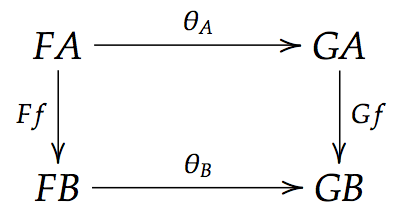
\includegraphics[width=0.4\linewidth]{diagrammeNaturel}
\begin{tikzcd}
	F(A) \arrow[r,"\theta_{A}"] \arrow[d,"F(f)"] & G(A) \arrow[d,"G(f)"] \\
	F(B) \arrow[r,"\theta_{B}"] & G(B)
\end{tikzcd}

}
\noindent
On note $\theta : F \Rightarrow G$, voire $\theta : F \Rightarrow G : \Ccal \longrightarrow \Dcal$.
\end{df}




\begin{df}
Soit une cat�gorie,
un morphisme $f:A\to B$ est un \textbf{\emph{isomorphisme}} s'il existe un morphisme $f^{-1}:B\to A$ tel que $f^{-1}\circ f=id_{A}$ et $f\circ f^{-1}=id_{B}$.
\end{df}


% def cat�gorie mono�dale
\begin{df}
Une \textbf{\emph{cat�gorie mono�dale}} est une cat�gorie $\Ccal$ munie d'un bifoncteur \\${\otimes:\Ccal\times\Ccal \longrightarrow \Ccal}$ (pour lequel on utilise une notation infixe) avec d'un objet particulier $e$, %tel que les morphismes suivants existent
%
%\begin{itemize}
%\item
%pour tous objets $A$, $B$, $C$, un isomorphisme naturel
%%\linebreak
%${\alpha_{A,B,C} : (A\otimes B)\otimes C \to A\otimes(B\otimes C)}$ permettant de parler d'associativit� ;
%\item
%pour tout objet $A$, des isomorphismes naturels ${\lambda_{A}:e\otimes A\to A}$ et ${\rho_{A}:A\otimes e\to A}$ %justifiant le nom d'\textbf{unit�} pour $e$ ;
%permettant d'appeler $e$ l'objet \textbf{unit�} ;
%\end{itemize}
telle qu'il existe des \textbf{isomorphismes naturels}
\begin{itemize}
\item
${\alpha_{A,B,C} : (A\otimes B)\otimes C \to A\otimes(B\otimes C)}$, permettant de parler d'associativit� ;
\item
${\lambda_{A}:e\otimes A\to A}$ ;
\item
${\rho_{A}:A\otimes e\to A}$,
permettant avec le pr�c�dent d'appeler $e$ l'objet \textbf{unit�} ;
\end{itemize}

\noindent
et tel que les diagrammes suivants commutent pour tous objets $A$, $B$, $C$, $D$. 

%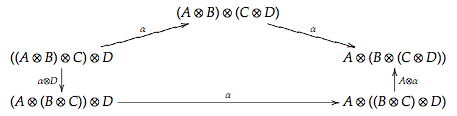
\includegraphics[width=\linewidth]{diagrammeMonoidalePenta}
%{\centering
%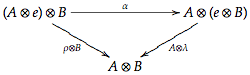
\includegraphics[width=0.5\linewidth]{diagrammeMonoidaleTri}
%			
%}
{\centering
\begin{tikzcd}
	& (A\otimes B)\otimes(C\otimes D) \arrow[rd,"\alpha_{A,B,C\otimes D}"] & \\
	((A\otimes B)\otimes C)\otimes D 
			\arrow[ru,"\alpha_{A\otimes B,C,D}"] 
			\arrow[d,"\alpha_{A,B,C}\otimes id_{D}"] 
		& & A\otimes(B\otimes(C\otimes D)) \\
	(A\otimes(B\otimes C)\otimes D 
			\arrow[rr,"\alpha_{A,B\otimes C,D}"]
		& & A\otimes((B\otimes C)\otimes D)
			\arrow[u,"id_{A}\otimes\alpha_{B,C,D}"]
\end{tikzcd}
\begin{tikzcd}
	(A\otimes e)\otimes B
			\arrow[rr,"\alpha_{A,e,B}"]
			\arrow[rd,"\rho_{A}\otimes id_{B}"]
		& & A\otimes(e\otimes B)
			\arrow[ld,"id_{A}\otimes\lambda_{B}"] \\
	& A\otimes B &
\end{tikzcd}
			
}
\noindent
Ces diagrammes sont appel�s \emph{diagrammes pentagonal} et \emph{triangulaire}. Leur commutativit� est la \emph{propri�t� de coh�rence}.
%On a omis les indices de $\alpha$, $\lambda$, $\rho$ et �crit $A$ pour $id_{A}$ : par exemple, comprendre $\alpha\otimes D$ comme $\alpha_{A,B,C}\otimes id_{A}$.
%On omet souvent les indices de $\alpha$, $\lambda$, $\rho$ lorsqu'il n'y a pas d'ambigu�t�. Ici, on �crit aussi $A$ pour $id_{A}$ : par exemple, comprendre $\alpha\otimes D$ comme ${\alpha_{A,B,C}\otimes id_{A}}$.

\vspace{2mm}

\noindent\textbf{Pr�cision.} On parle d'isomorphismes naturels car il y a bien des transformations naturelles associ�es. En fait la condition sur $\alpha$ est $\alpha : F \Rightarrow G :\Ccal\times\Ccal\times\Ccal \longrightarrow \Ccal$ avec $F:(x,y,z) \mapsto (x\otimes y)\otimes z$ et $G:(x,y,z) \mapsto x\otimes(y\otimes z)$ o� $x$, $y$, $z$ sont trois objets ou trois morphismes de $\Ccal$. On �crit $\alpha_{A,B,C}$ pour $\alpha_{(A,B,C)}$. Les $\alpha_{A,B,C}$ sont bien des morphismes de $\Ccal$, qui est la cat�gorie d'arriv�e de $F$ et $G$. On veut aussi ${\lambda : (e\otimes\bullet) \Rightarrow Id_{\Ccal} : \Ccal \longrightarrow \Ccal}$ o� $(e\otimes\bullet) : \left\{
\begin{array}{l}
	A \mapsto e\otimes A \\
	f \mapsto id_{e}\otimes f
\end{array}
\right.$ et o� $Id_{\Ccal}$ est le foncteur identit� sur $\Ccal$. Il y a une condition similaire pour $\rho$.


\end{df}


%L'op�rateur $\otimes$ qu'on a d�finit sur les d�notations de formules puis sur les d�notations de preuves constitue un \emph{bifoncteur} de la cat�gorie $\CProofs$, c'est-�-dire un foncteur $\otimes : \Ccal\times\Ccal \longrightarrow \Ccal$. $\Ccal$ munie de $\otimes$ est presque une \textbf{cat�gorie mono�dale} avec comme objet unit� $[\1]$, la d�notation de la formule $\1$, �l�ment neutre pour le connecteur $\otimes$.

On munit la cat�gorie $\CProofs$ du bifoncteur $\otimes$ et on choisit comme objet unit� $[\1]$, la d�notation de la formule $\1$, �l�ment neutre pour le connecteur $\otimes$. On obtient une \textbf{cat�gorie mono�dale}, ou presque une cat�gorie mono�dale, selon les choix effectu�s pour d�finir le proc�d� d'�limination de la coupure.
%La cat�gorie $\Ccal$ munie du bifoncteur $\otimes$ est presque une \textbf{cat�gorie mono�dale} avec comme objet unit� $[\1]$, la d�notation de la formule $\1$, �l�ment neutre pour le connecteur $\otimes$.
En effet, on peut d�finir des morphismes $\alpha_{A,B,C}$, $\lambda_{A}$, $\rho_{A}$ comme les d�notations des preuves suivantes\\

\def\alphaABC{
$\alpha_{A,B,C}$ :
	\AXC{}
	\RightLabel{$(id)$}
	\UIC{$A\vdash A$}
	  \AXC{}
	  \RightLabel{$(id)$}
	  \UIC{$B\vdash B$}
	    \AXC{}
	    \RightLabel{$(id)$}
	    \UIC{$C\vdash C$}
	  \RightLabel{$(\otimes R)$}
	  \BIC{$B,C \vdash B\otimes C$}
	\RightLabel{$(\otimes R)$}
	\BIC{$A,B,C \vdash A\otimes(B\otimes C)$}
	\RightLabel{$(\otimes L)$}
	\UIC{$A\otimes B,C \vdash A\otimes(B\otimes C)$}
	\RightLabel{$(\otimes L)$}
	\UIC{$(A\otimes B)\otimes C \vdash A\otimes(B\otimes C)$}
\DP
}

\def\lambdaA{
$\lambda_{A}$ :
	\AXC{}
	\RightLabel{$(id)$}
	\UIC{$A\vdash A$}
	\RightLabel{$(\1 L)$}
	\UIC{$\1,A\vdash A$}
	\RightLabel{$(\otimes L)$}
	\UIC{$\1\otimes A\vdash A$}
\DP
}

\def\rhoA{
$\rho_{A}$ : 
	\AXC{}
	\RightLabel{$(id)$}
	\UIC{$A\vdash A$}
	\RightLabel{$(\1 L)$}
	\UIC{$A,\1\vdash A$}
	\RightLabel{$(\otimes L)$}
	\UIC{$A\otimes\1\vdash A$}
\DP
}

%\begin{tabular}{p{0.5\linewidth}p{0.5\linewidth}}
%	\multicolumn{2}{l}{\quad\; \alphaABC} \\ \\
%	\lambdaA & \rhoA
%\end{tabular}
% alpha : \qquad\qquad, 2 autres : \quad

\noindent
\resizebox{\linewidth}{!}{
\alphaABC \quad \lambdaA \quad \rhoA
}

\

\noindent
Il s'agit bien de transformations naturelles, et on a bien la propri�t� de coh�rence.
\idees{d�monstrations, ou au moins explications, exemples de preuves �quivalentes ?}
%
La d�finition d'une \emph{cat�gorie mono�dale} exige que ces morphismes $\alpha$, $\lambda$, $\rho$ soient des isomorphismes. On n'�crit plus les indices, qui sont toujours les m�mes. On peut d�finir des morphismes naturels $\bar\alpha_{A,B,C} : A\circ(B\circ C) \to (A\circ B)\circ C$ \,,\; $\bar\lambda_{A} : A \to e\circ A$ \,,\; $\bar\rho_{A} : A \to A\circ e$\,, par exemple $\bar\lambda_{A}$ est la d�notation de 
\resizebox{3cm}{!}{
	\AXC{}
	\RightLabel{$(\1 R)$}
	\UIC{$\vdash \1$}
		\AXC{}
		\RightLabel{$(id)$}
		\UIC{$A\vdash A$}
	\RightLabel{$(\otimes R)$}
	\BIC{$A\vdash \1\otimes A$}
\DP
}
. On pense naturellement � ces morphismes quand on cherche des inverses de $\alpha$, $\lambda$ et $\rho$. On a bien ${\lambda\circ\bar\lambda = id_{A}}$ et ${\rho\circ\bar\rho=id_{A}}$. En revanche, si on consid�re un p.�.c. ``strict'', on n'a aucune des �galit�s suivantes : ${\bar\lambda\circ\lambda = id_{e\circ A}}$\,,\; ${\bar\rho\circ\rho=id_{A\circ e}}$\,,\; ${\bar\alpha\circ\alpha=id_{(A\circ B)\circ C}}$\,,\; ${\alpha\circ\bar\alpha=id_{A\circ(B\circ C)}}$\,. Si on consid�re au contraire la version plus ``large'' du p.�.c., on a bien toutes ces �galit�s. Les transformations autoris�es qui ont �t� ajout�es au p.�.c. strict pour obtenir cette version large sont d'ailleurs express�ment choisies pour satisfaire ces �galit�s. Dans la suite, on suppose toujours qu'on a choisi la version ``large'' du p.�.c., donc $\CProofs$ est bien une cat�gorie mono�dale.
%On obtient alors que $\CProofs$ est une \textbf{cat�gorie mono�dale}. Dans la suite, on se met toujours dans ce cas



%En revanche, si on consid�re un p.�.c. ``strict'', ces morphismes $\alpha$, $\lambda$, $\rho$ ne sont pas des isomorphismes. On n'�crit plus les indices, qui sont toujours les m�mes. On peut d�finir des morphismes naturels $\bar\alpha_{A,B,C} : A\circ(B\circ C) \to (A\circ B)\circ C$ \,,\; $\bar\lambda_{A} : A \to e\circ A$ \,,\; $\bar\rho_{A} : A \to A\circ e$\,, par exemple $\bar\lambda_{A}$ est la d�notation de 
%\resizebox{3cm}{!}{
%	\AXC{}
%	\RightLabel{$(\1 R)$}
%	\UIC{$\vdash \1$}
%		\AXC{}
%		\RightLabel{$(id)$}
%		\UIC{$A\vdash A$}
%	\RightLabel{$(\otimes R)$}
%	\BIC{$A\vdash \1\otimes A$}
%\DP
%}
%. On pense naturellement � ces morphismes quand on cherche des inverses de $\alpha$, $\lambda$ et $\rho$. On a bien ${\lambda\circ\bar\lambda = id_{A}}$ et ${\rho\circ\bar\rho=id_{A}}$, mais on n'a aucune des �galit�s suivantes : ${\bar\lambda\circ\lambda = id_{e\circ A}}$\,,\; ${\bar\rho\circ\rho=id_{A\circ e}}$\,,\; ${\bar\alpha\circ\alpha=id_{(A\circ B)\circ C}}$\,,\; ${\alpha\circ\bar\alpha=id_{A\circ(B\circ C)}}$\,.
%
%Cependant en ajoutant des transformations ...



%\def\noninverseUn{
%	\AXC{}
%	\RightLabel{$(id)$}
%	\UIC{$A\vdash A$}
%	\RightLabel{$(\1 L)$}
%	\UIC{$A,\1\vdash A$}
%	\RightLabel{$(\otimes L)$}
%	\UIC{$A\otimes\1\vdash A$}
%		\AXC{}
%		\RightLabel{$(id)$}
%		\UIC{$A\vdash A$}
%			\AXC{}
%			\RightLabel{$(\1 R)$}
%			\UIC{$\vdash \1$}
%		\RightLabel{$(\otimes R)$}
%		\BIC{$A\vdash A\otimes\1$}
%	\RightLabel{$(cut)$}
%	\BIC{$A\otimes\1\vdash A\otimes\1$}
%	\noLine
%	\UIC{}
%	\noLine
%	\UIC{$p_{1}$}
%\DP
%}
%\def\noninverseDeux{
%	\AXC{}
%	\RightLabel{$(id)$}
%	\UIC{$A\vdash A$}
%	\RightLabel{$(\1 L)$}
%	\UIC{$A,\1\vdash A$}
%	\RightLabel{$(\otimes L)$}
%	\UIC{$A\otimes\1\vdash A$}
%		\AXC{}
%		\RightLabel{$(\1 R)$}
%		\UIC{$\vdash \1$}
%	\RightLabel{$(\otimes R)$}
%	\BIC{$A\otimes\1\vdash A\otimes\1$}
%	\noLine
%	\UIC{}
%	\noLine
%	\UIC{$p_{2}$}
%\DP
%}
%\def\noninverseTrois{
%	\AXC{}
%	\RightLabel{$(id)$}
%	\UIC{$A\vdash A$}
%		\AXC{}
%		\RightLabel{$(id)$}
%		\UIC{$\1 \vdash \1$}
%	\RightLabel{$(\otimes R)$}
%	\BIC{$A,\1\vdash A\otimes\1$}
%	\RightLabel{$(\otimes L)$}
%	\UIC{$A\otimes\1\vdash A\otimes\1$}
%	\noLine
%	\UIC{}
%	\noLine
%	\UIC{$p_{3}$}
%\DP
%}
%\noindent
%\resizebox{\linewidth}{!}{
%%\begin{tabular}{ccc}
%%	\noninverseUn & \noninverseDeux & \noninverseTrois
%%\end{tabular}
%\noninverseUn \quad \noninverseDeux \quad \noninverseTrois
%}


%


\subsection{\'Echange et cat�gorie mono�dale sym�trique}

\def\sizesymetrie{0.27\textwidth}
\begin{floatingfigure}[r]{\sizesymetrie}
\centering
\resizebox{\sizesymetrie}{!}{
	\AXC{}
	\RightLabel{$(id)$}
	\UIC{$B\vdash B$}
		\AXC{}
		\RightLabel{$(id)$}
		\UIC{$A\vdash A$}
	\RightLabel{$(\otimes R)$}
	\BIC{$B,A \vdash B\otimes A$}
	\RightLabel{$(exchange)$}
	\UIC{$A,B \vdash B\otimes A$}
	\RightLabel{$(\otimes L)$}
	\UIC{$A\otimes B \vdash B\otimes A$}
\DP
}
\\
\end{floatingfigure}

La logique lin�aire est commutative : la r�gle d'�change ... permet de construire la preuve canonique de $A\otimes B \vdash B\otimes A$ ci-contre. On peut alors ajouter un nouvel isomorphisme naturel � $\CProofs$ pour en faire une cat�gorie mono�dale sym�trique. Des variantes ``non commutatives'' ont �t� �tudi�es dans la litt�rature, o� la r�gle d'�change est supprim�e ou affaiblie. %Dans ce dernier cas, on peut parfois obtenir une cat�gorie mono�dale non pas sym�trique, mais \emph{tress�e}
Dans ce dernier cas, on peut parfois obtenir quand m�me une cat�gorie mono�dale tress�e.

\vspace{3mm}
%\

\begin{df}
Soit $\Ccal$ une cat�gorie mono�dale, avec les notations pr�c�dentes. C'est une \textbf{\emph{cat�gorie mono�dale tress�e}} s'il existe un \textbf{isomorphisme naturel} $\gamma_{A,B} : A\otimes B \to B\otimes A$ tel que les \emph{diagrammes hexagonaux} suivants commutent.
\vspace{1mm}

\noindent
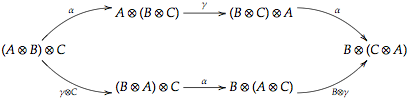
\includegraphics[width=0.48\linewidth]{diagrammeHexa1}
\quad
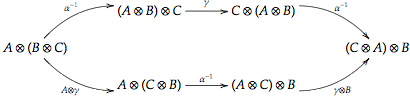
\includegraphics[width=0.48\linewidth]{diagrammeHexa2}

\begin{tikzcd}
	& A\otimes(B\otimes C)
		\arrow[r,"\alpha_{A,e,B}"]
	& (B\otimes C)\otimes A
& \\
	(A\otimes B)\otimes C
		\arrow[ru,"\alpha_{A,e,B}"]
		\arrow[ru,"\alpha_{A,e,B}"]	
	& & & B\otimes(C\otimes A)
%	(A\otimes e)\otimes B
%			\arrow[rr,"\alpha_{A,e,B}"]
%			\arrow[rd,"\rho_{A}\otimes id_{B}"]
%		& & A\otimes(e\otimes B)
%			\arrow[ld,"id_{A}\otimes\lambda_{B}"] \\
%	& A\otimes B &
\end{tikzcd}

\end{df}



\begin{df}
Soit $\Ccal$ une cat�gorie mono�dale tress�e, avec les notations pr�c�dentes. C'est une \textbf{\emph{cat�gorie mono�dale sym�trique}} si pour tous objets $A$, $B$, on a $\gamma_{B,A}=\gamma_{A,B}^{-1}$. Dans ce cas, on n'a pas besoin de v�rifier la commutativit� du second diagramme de la d�finition pr�c�dente, qui est entra�n�e par la commutativit� du premier diagramme appliqu�e � $\gamma_{B,A}$.
\end{df}

Dans $\Ccal$, on d�finit $\gamma_{A,B}$ comme la d�notation de la preuve canonique de $A\otimes B \vdash B\otimes A$ donn�e pr�c�demment. %Si on a assoupli l'�quivalence d'�limination de la coupure pour que $\Ccal$ soit une cat�gorie mono�dale, on 
On obtient alors une \textbf{cat�gorie mono�dale sym�trique}.
\idees{vrai ? d�monstrations, explications, exemples ?}


%



\subsection{Implication lin�aire et cat�gorie mono�dale ferm�e}

Int�ressons-nous maintenant � l'implication lin�aire $\multimap$. Ce connecteur logique induit encore une fois un op�rateur sur les d�notations de formules, qui a un sens en th�orie des cat�gories.

\begin{df}
Soit $\Ccal$ une cat�gorie mono�dale, toujours avec les m�mes notations. Une \textbf{\emph{structure ferm�e � gauche}} sur $\Ccal$ consiste en un op�rateur $\multimap$ sur les objets et pour tous objets $A$, $B$, un morphisme $eval_{A,B} : A\otimes(A\multimap B)\to B$, v�rifiant la propri�t� d'universalit� suivante : pour tout objet $X$ et tout morphisme $f:A\otimes X\to B$, il existe un unique morphisme $h:X\to A\multimap B$ tel que le diagramme suivant commute.

\noindent
{\centering
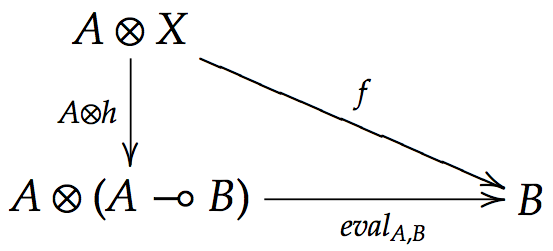
\includegraphics[width=4cm]{diagrammeFermeeGauche}

}
On dit alors que $\Ccal$ est une \textbf{\emph{cat�gorie mono�dale ferm�e}}.
\end{df}


\def\sizesymetrie{0.3\textwidth}
\begin{floatingfigure}[r]{\sizesymetrie}
\centering
\resizebox{\sizesymetrie}{!}{
	\AXC{}
	\RightLabel{$(id)$}
	\UIC{$A\vdash A$}
		\AXC{}
		\RightLabel{$(id)$}
		\UIC{$B\vdash B$}	
	\RightLabel{$(\multimap L)$}
	\BIC{$A,(A\multimap B) \vdash B$}
	\RightLabel{$(\otimes L)$}
	\UIC{$A\otimes(A\multimap B) \vdash B$}
\DP
}
\\
\end{floatingfigure}

On munit $\CProofs$ de l'op�rateur $\multimap$ sur les d�notations de formules correspondant � l'implication lin�aire. On d�finit $eval_{A,B}$ comme la d�notation de la preuve ci-contre. On obtient alors une \textbf{cat�gorie mono�dale ferm�e}.
\idees{Est-ce vrai ? Est-ce qu'on peut expliquer facilement comment obtenir $h$ � partir de $f$ ?}


%





%%%%%%%%%%%%%%

\end{document}






\subsection{``Avec'' et produit cart�sien}


\subsection{Cat�gorie libre}







\pagebreak





% def cat�gorie
\begin{df}
Une \textbf{\emph{cat�gorie}} consiste en une collection d'\emph{objets} et une collection de \emph{morphismes}, cette derni�re munie d'une op�rations binaire partielle $\circ$ appel�e \emph{composition}, avec les propri�t�s suivantes.

\begin{itemize}

\item
\`A chaque morphisme $f$ est associ� un couple d'objets $(A,B)$ ; on �crit $f:A\to B$.
On dit que $A\to B$ est le \emph{type} de $f$, et que $f$ est un morphisme \emph{de} $A$ \emph{vers} $B$, et encore que $A$ est le \emph{domaine} ou la \emph{source} de $f$, et $B$ le \emph{codomaine} ou la \emph{cible} de $f$.

\item
Pour tous objets $A$, $B$, $C$ et morphismes $f$, $g$ tels que $f:A\to B$ et $g:B\to C$, le morphisme $g\circ f$ existe et $g\circ f:A\to C$.

\item
\textbf{Identit�.}
Pour tout objet $A$, il existe un morphisme particulier $id_{A}:A\to A$ appel� \emph{identiti� sur $A$}, tel que 
%pour tous objet $B$ et morphismes $f:B\to A$ et $g:A\to B$, $id_{A}\circ f=f$ et $g\circ id_{A}=g$.
pour tout objet $B$, pour tout $f:B\to A$, $id_{A}\circ f=f$ et pour tout $g:A\to B$, $g\circ id_{A}=g$.

\item
\textbf{Associativit�.}
Pour tous $f:A\to B$, $g:B\to C$, $h:C\to D$, on a $h\circ(g\circ f) = (h\circ g)\circ f$.

\end{itemize}
\end{df}

On d�signe souvent une cat�gorie par la collection de ses objets.


% def cat�gorie mono�dale
\begin{df}
%Une \textbf{\emph{cat�gorie mono�dale}} est une cat�gorie $\C$ munie d'un bifoncteur ${\otimes:\C\times\C \longrightarrow \C}$ tel que
%
%\begin{itemize}
%%\item
%%pour tous objets $A$, $B$, $C$, il existe une isomorphisme naturel d'associativit�
%%\linebreak
%%${\alpha_{A,B,C} : (A\otimes B)\otimes C \to A\otimes(B\otimes C)}$ ;
%%\item
%%il existe un objet $e$, unitaire
%\item
%une \textbf{associativit�} est fournie par un morphisme naturel pour tous objets $A$, $B$, $C$ : ${\alpha_{A,B,C} : (A\otimes B)\otimes C \to A\otimes(B\otimes C)}$ ;
%\item
%il existe un objet $e$ \textbf{unitaire} gr�ce � des morphismes naturels pour tout objet $A$ : ${\lambda_{A}:e\otimes A\to A}$ et ${\rho_{A}:A\otimes e\to A}$.
% 
%\end{itemize}

Une \textbf{\emph{cat�gorie mono�dale}} est une cat�gorie $\Ccal$ munie d'un bifoncteur ${\otimes:\Ccal\times\Ccal \longrightarrow \Ccal}$ et d'un objet $e$, tel que les morphismes suivants existent

\begin{itemize}
\item
pour tous objets $A$, $B$, $C$, un isomorphisme
%\linebreak
${\alpha_{A,B,C} : (A\otimes B)\otimes C \to A\otimes(B\otimes C)}$ permettant de parler d'associativit� ;
\item
pour tout objet $A$, des isomorphismes ${\lambda_{A}:e\otimes A\to A}$ et ${\rho_{A}:A\otimes e\to A}$ justifiant le nom d'\textbf{unit�} pour $e$ ;
\end{itemize}

\noindent
et tel que les diagrammes suivants commutent pour tous objets $A$, $B$, $C$, $D$. On a omis les indices de $\alpha$, $\lambda$, $\rho$ et �crit $A$ pour $id_{A}$ : par exemple, comprendre $\alpha\otimes D$ comme $\alpha_{A,B,C}\otimes id_{A}$.

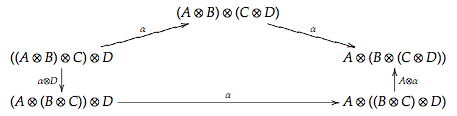
\includegraphics[width=\linewidth]{diagrammeMonoidalePenta}
\centering{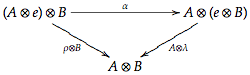
\includegraphics[width=0.5\linewidth]{diagrammeMonoidaleTri}}

\end{df}





\pagebreak

\`A chaque preuve $\pi$ on associe une \emph{d�notation} $[\pi]$, qu'on veut invariante par �limination de la coupure.

\

Les objets sont les formules et les morphismes sont des d�notations de preuves. Les morphismes d'une formule $A$ vers une formule $B$ sont les d�notations des diff�rentes preuves du s�quent $A\vdash B$ (si le s�quent n'est pas prouvable, il n'y en a pas).

Soit $A$, $B$, $C$ des formules, $\pi_{1}$ une preuve de $A\vdash B$ et $\pi_{2}$ une preuve de $B\vdash C$. On d�finit $[\pi_{2}]\circ[\pi_{1}]$ comme la d�notation de la preuve suivante de $A\vdash C$
\begin{prooftree}
	\AXC	{$\pi_{1}$}
	\noLine
	\UIC{$A\vdash B$}
	\AXC	{$\pi_{2}$}
	\noLine
	\UIC{$B\vdash C$}
	\RightLabel{$(cut)$}
	\BIC{$A\vdash C$}
\end{prooftree}

L'identit� $id_{A}$ sur une formule $A$ est la d�notation de la preuve
{\centerAlignProof
	\AXC	{}
	\RightLabel{$(Id)$}
	\UIC{$A\vdash A$}
	\DP
}.
Soit $\pi$ une preuve de $A\vdash B$, l'�limination de la coupure transforme la preuve
\\
\begin{center}
	\AXC	{}
	\RightLabel{$(Id)$}
	\UIC{$A\vdash A$}
	\AXC	{$\pi$}
	\noLine
	\UIC{$A\vdash B$}
	\RightLabel{$(cut)$}
	\BIC{$A\vdash B$}
	\DP
\qquad\qquad en \qquad\qquad
	\AXC	{$\pi$}
	\noLine
	\UIC{$A\vdash B$}
	\DP
\end{center}

\noindent
donc on a bien $[\pi]\circ id_{A}=[\pi]$. De m�me pour $\pi$ une preuve de $B\vdash A$, on a $id_{A}\circ[\pi]=[\pi]$.

L'associativit� vient de ce que les preuves
\\
\begin{center}
	\AXC	{$\pi_{1}$}
	\noLine
	\UIC{$A\vdash B$}
	\AXC	{$\pi_{2}$}
	\noLine
	\UIC{$B\vdash C$}
	\RightLabel{$(cut)$}
	\BIC{$A\vdash C$}
	\AXC	{$\pi_{3}$}
	\noLine
	\UIC{$C\vdash D$}
	\RightLabel{$(cut)$}
	\BIC{$A\vdash D$}
	\DP
\quad et \quad
	\AXC	{$\pi_{1}$}
	\noLine
	\UIC{$A\vdash B$}
	\AXC	{$\pi_{2}$}
	\noLine
	\UIC{$B\vdash C$}
	\AXC	{$\pi_{3}$}
	\noLine
	\UIC{$C\vdash D$}
	\RightLabel{$(cut)$}
	\BIC{$B\vdash D$}
	\RightLabel{$(cut)$}
	\BIC{$A\vdash D$}
	\DP
\end{center}

\noindent
sont �quivalentes � �limination de la coupure pr�s.







\end{document}



\pagebreak


\documentclass[11pt, openany]{article}
%\usepackage{pstricks,pstricks-add,pst-math,pst-xkey}
\usepackage[frenchb]{babel}
%\usepackage{slashbox}
\usepackage{graphicx}
\usepackage{amsmath,amssymb,amstext}
\usepackage[latin1]{inputenc}
\usepackage[OT1]{fontenc}
%\usepackage{fancybox}
\usepackage{a4wide}
%\usepackage{fancyvrb}
\usepackage{pgf,tikz} %arbres
%\usetikzlibrary{arrows}
\usepackage{xcolor}
%\usepackage{multicol}
%\usepackage[cm]{fullpage}
\usepackage{amsthm} %pour les th�or�mes sans num�ro
\usepackage{array,multirow,makecell}
\usepackage{mathrsfs}

\usepackage{floatflt}

\usepackage{bussproofs}\EnableBpAbbreviations


\bibliographystyle{ieeetr}  


\newcounter{moncompteur}
\newtheorem{q}[moncompteur]{\textbf{Question}}{}
\newtheorem{prop}[moncompteur]{\textbf{Proposition}}{}
\newtheorem{df}[moncompteur]{\textbf{D�finition}}{}
\newtheorem*{df*}{\textbf{D�finition}}{}
\newtheorem{rem}[moncompteur]{\textbf{Remarque}}{}
\newtheorem{theo}[moncompteur]{\textbf{Th�or�me}}{}
\newtheorem*{theo*}{\textbf{Th�or�me}}{}
\newtheorem{conj}[moncompteur]{\textbf{Conjecture}}{}
\newtheorem{cor}[moncompteur]{\textbf{Corollaire}}{}
\newtheorem{lm}[moncompteur]{\textbf{Lemme}}{}
\newtheorem*{lm*}{\textbf{Lemme}}{}
%\newtheorem{nota}[moncompteur]{ \textbf{Notation}}{}
%\newtheorem{conv}[moncompteur]{ \textbf{Convention}}{}
\newtheorem{exa}[moncompteur]{\textbf{Exemple}}{}
\newtheorem{ex}[moncompteur]{\textbf{Exercice}}{}
%\newtheorem{app}[moncompteur]{ \textbf{Application}}{}
%\newtheorem{prog}[moncompteur]{ \textbf{Algorithme}}{}
%\newtheorem{hyp}[moncompteur]{ \textbf{Hypoth�se}}{}
%\newenvironment{dem}{\noindent\textbf{Preuve}\\}{\flushright$\blacksquare$\\}
%\newenvironment{dem}{\noindent\textbf{Preuve.} }{\hfill$\blacksquare$\\}

%\newenvironment{myindentpar}[1]%
%{\begin{list}{}%
%         {\setlength{\leftmargin}{#1}}%
%         \item[]%
%}
%{\end{list}}



%\newcommand{\R}{\mathbb{R}}
%\newcommand{\K}{\mathbb{K}}
%\newcommand{\N}{\mathbb{N}}
%\newcommand{\Z}{\mathbb{Z}}
%\newcommand{\C}{\mathbb{C}}
%\newcommand{\U}{\mathbb{U}}
%\newcommand{\Q}{\mathbb{Q}}
%\newcommand{\card}{\mathrm{card}}


\newcommand{\s}{\sigma}
%\newcommand{\l}{\lambda}
%\newcommand{\a}{\alpha}
%\newcommand{\r}{\rho}

%m�moire
\newcommand{\Ccal}{\mathcal{C}}
\newcommand{\Dcal}{\mathcal{D}}
\newcommand{\1}{\boldsymbol{1}}
\newcommand{\CProofs}{
%?\mathcal{C}?
\mathcal{CP}
}
%

\newcommand{\subsectionDescription}[1]{
\addtocontents{toc}{%\textit{
%\qquad\qquad
\hangindent=3.5\parindent \hangafter=0
\noindent
#1
}%}
}


\newcommand{\idees}[1]{
\textsf{(#1)}
}



%stage
\newcommand{\LK}{$\mathbf{LK}$}
\newcommand{\LJ}{$\mathbf{LJ}$}
\newcommand{\LJT}{$\mathbf{LJT}$}
\newcommand{\LSJ}{$\mathbf{LSJ}$}
\newcommand{\LSJn}{$\mathbf{LSJ\boldsymbol\ell}$}


\newcommand{\Sig}{\mathfrak S}
\newcommand{\G}{\Gamma}
\newcommand{\D}{\Delta}
\newcommand{\Th}{\Theta}
\newcommand{\Gp}{\Gamma}
\newcommand{\Dp}{\Delta}
\newcommand{\Gt}{\widetilde\Gamma}
\newcommand{\Dt}{\widetilde\Delta}

\newcommand{\imp}{\to\negthickspace}

\newcommand{\surj}{
%\mathrm{surj}
\boldsymbol
\Phi
}
\newcommand{\To}{\Rightarrow}
\newcommand{\forget}{\mathsf{forget}}



\newcommand{\autour}[5]{
^{#2}_{#3}#1^{#4}_{#5}
}




\begin{document}
\renewcommand{\labelitemi}{$\diamond$}
\vspace{2cm}~~\\


%regles et instances
\def\regle{
\def\defaultHypSeparation{\hskip .05in}
	\AXC	{$prem_{1}$}
	\AXC	{...}
	\AXC	{$prem_{p}$}
	\RightLabel{$(\mathcal R)$}
	\TIC{$concl$}
	\DP
}
\def\instance{
\def\defaultHypSeparation{\hskip .05in}
	\AXC	{$\s_{1}$}
	\AXC	{...}
	\AXC	{$\s_{p}$}
	\RightLabel{$(\mathcal R)$}
	\TIC{$\s$}
	\DP
}
\def\instanceAx{
\centerAlignProof
	\AXC	{\qquad}
	\RightLabel{$(\mathcal A)$}
	\UIC{$\s$}
	\DP
}
\def\instancedeux{
\def\defaultHypSeparation{\hskip .05in}
	\AXC	{$\s_{1}$}
	\AXC	{$\s_{2}$}
	\BIC{$\s$}
	\DP
}


%LJ
%LJ, axiomes
\def\LJid{
	\AXC	{}
	\RightLabel{$(id)$}
	\UIC{$A,\G \To A$}
	\DP
}
\def\LJbotL{
	\AXC	{}
	\RightLabel{$(\bot L)$}
	\UIC{$\bot,\G \To D$}
	\DP
}
%LJ,r�gles logiques
\def\LJetL{
	\AXC	{$A,B,\G \To D$}
	\RightLabel{$(\land L)$}
	\UIC{$A\land B,\G \To D$}
	\DP
}
\def\LJetR{
	\AXC	{$\G \To A$}
	\AXC	{$\G \To B$}
	\RightLabel{$(\land R)$}
	\BIC{$\G \To A\land B$}
	\DP
}
\def\LJouL{
	\AXC	{$A,\G \To D$}
	\AXC	{$B,\G \To D$}
	\RightLabel{$(\lor L)$}
	\BIC{$A\lor B,\G \To D$}
	\DP
}
\def\LJouRun{
	\AXC	{$\G \To A$}
	\RightLabel{$(\lor R_{1})$}
	\UIC{$\G \To A\lor B$}
	\DP
}
\def\LJouRdeux{
	\AXC	{$\G \To B$}
	\RightLabel{$(\lor R_{2})$}
	\UIC{$\G \To A\lor B$}
	\DP
}
\def\LJimpL{
	\AXC	{$\G \To A$}
	\AXC	{$B,\G \To D$}
	\RightLabel{$(\to L)$}
	\BIC{$A\to B,\G \To D$}
	\DP
}
\def\LJimpR{
	\AXC	{$A,\G \To B$}
	\RightLabel{$(\to R)$}
	\UIC{$\G \To A\to B$}
	\DP
}
%LJ, r�gles structurelles
\def\LJechange{
	\AXC	{$\G_{1},A,B,\G_{2} \To D$}
	\RightLabel{$(permut.\ L)$}
	\UIC{$\G_{1},B,A,\G_{2} \To D$}
	\DP
}
\def\LJcontraction{
	\AXC	{$A,A,\G \To D$}
	\RightLabel{$(contraction\ L)$}
	\UIC{$A,\G \To D$}
	\DP
}
\def\LJweakening{
	\AXC	{$\G \To D$}
	\RightLabel{$(weakening\ L)$}
	\UIC{$A,\G \To D$}
	\DP
}
%LJ, coupure
\def\LJcut{
	\AXC	{$\G_{1} \To A$}
	\AXC	{$A,\G_{2} \To D$}
	\RightLabel{$(cut)$}
	\BIC{$\G_{1},\G_{2} \To D$}
	\DP
}


%LK
\def\LKetR{
	\AXC	{$\G \To A,\D$}
	\AXC	{$\G \To B,\D$}
	\RightLabel{$(\land R)$}
	\BIC{$\G \To A\land B,\D$}
	\DP
}
\def\LKouR{
	\AXC	{$\G \To A,B,\D$}
	\RightLabel{$(\lor R)$}
	\UIC{$\G \To A\lor B,\D$}
	\DP
}

\def\LKTiersExclu{
	\AXC	{}
	\RightLabel{(id)}
	\UIC	{$A \To A, \bot$}
	\RightLabel{$(\to R)$}
	\UIC	{$\To A, (A\to\bot)$}
	\RightLabel{$(\lor R)$}
	\UIC{$\To A\lor (A\to\bot)$}
	\DP
}


%LJ ajustement
\def\LJimpLcontr{
	\AXC	{$\G,A\to B \To A$}
	\AXC	{$\G,B \To D$}
	\RightLabel{$(\to L)$}
	\BIC{$\G,A\to B \To D$}
	\DP
}
\def\LJimpLcontrA{
	\AXC	{$\G,A\to B \To A$}
	\AXC	{$\G,B \To A$}
	\RightLabel{$(\to L)$}
	\BIC{$\G,A\to B \To A$}
	\DP
}

\def\LJnnTiersExclu{
%	\AXC	{}
%	\RightLabel{id}
%	\UIC	{$A \To A, \bot$}
%	\RightLabel{$\to R$}
%	\UIC	{$\To A, (A\to\bot)$}
%	\RightLabel{$\lor R$}
	
	\AXC	{}
	\RightLabel{(id)}
	\UIC	{$A \;\To\; A$}
	\RightLabel{$(\lor R_{1})$}
	\UIC	{$A \;\To\; A\lor (A\to\bot)$}
	
		\AXC	{}
		\RightLabel{$(\bot L)$}
		\UIC	{$\bot,A \;\To\; \bot$}
	
	\RightLabel{$(\to L)$}
	\BIC	{$A,(A\lor (A\to\bot))\to\bot \;\To\; \bot$}
	\RightLabel{$(\to R)$}
	\UIC	{$(A\lor (A\to\bot))\to\bot \;\To\; A\to\bot$}
	\RightLabel{$(\lor R_{2})$}
	\UIC	{\colorbox{yellow}{$(A\lor (A\to\bot))\to\bot \;\To\; A\lor (A\to\bot)$}}
	
		\AXC	{}
		\RightLabel{$(\bot L)$}
		\UIC	{$\bot,(A\lor (A\to\bot))\to\bot \;\To\; \bot$}
	
	\RightLabel{$(\to L)$}
	\BIC	{$(A\lor (A\to\bot))\to\bot \,,\; (A\lor (A\to\bot))\to\bot \;\To\; \bot$}
	\RightLabel{$(contraction\ L)$}
	\UIC	{$(A\lor (A\to\bot))\to\bot \;\To\; \bot$}
	\RightLabel{$(\to R)$}
	\UIC{$\;\To\; ((A\lor (A\to\bot))\to\bot)\to\bot$}
	\DP
}





%LJT
\def\LJTimpLun{
	\AXC	{$B,A,\G \;\To\; D$}
	\RightLabel{$(\to L_{1})$}
	\UIC{$A\to B, A,\G \;\To\; D$}
	\DP
}
\def\LJTimpLdeux{
	\AXC	{$A_{1}\to(A_{2}\to B) \,,\; \G \;\To\; D$}
	\RightLabel{$(\to L_{2})$}
	\UIC{$(A_{1}\land A_{2})\to B \,,\; \G \;\To\; D$}
	\DP
}

%%%%%%%%%%%%

%LSJ

\def\LSJfauxL{
	\AXC	{}
	\RightLabel{$(\bot L)$}
	\UIC{$\Th\,; \bot, \G \To \D$}
	\DP
}
\def\LSJid{
	\AXC	{}
	\RightLabel{$(id)$}
	\UIC{$\Th\,; A,\G \To A,\D$}
	\DP
}
\def\LSJetL{
	\AXC{$\Th\,; A, B,\G \To \D$}
	\RightLabel{$(\land L)$}
	\UIC{$\Th\,; A\land B,\G \To  \D$}
	\DP
}
\def\LSJetR{
	\AXC{$\Th\,; \G \To A,\D$}
	\AXC{$\Th\,; \G \To B,\D$}
	\RightLabel{$(\land R)$}
	\BIC{$\Th\,; \G \To A\land B,\D$}
	\DP
}
\def\LSJouL{
	\AXC{$\Th\,; A,\G \To \D$}
	\AXC{$\Th\,; B,\G \To \D$}
	\RightLabel{$(\lor L)$}
	\BIC{$\Th\,; A\lor B,\G \To \D$}
	\DP
}
\def\LSJouR{
	\AXC{$\Th\,; \G \To A,B,\D$}
	\RightLabel{$(\lor R)$}
	\UIC{$\Th\,; \G \To A\lor B,\D$}
	\DP
}
\def\LSJimpL{
	\AXC{$\Th\,; B,\G \To \D$}
	\AXC{$B,\Th\,; \G \To A,\D$}
	\AXC{$B\,; \Th,\G \To A$}
	\RightLabel{$(\to L)$}
	\TIC{$\Th\,; A\to B,\G \To \D$}
	\DP
}
\def\LSJimpR{
	\AXC{$\Th\,; A,\G \To B,\D$}
	\AXC{$\emptyset\,; A,\Th,\G \To B$}
	\RightLabel{$(\to R)$}
	\BIC{$\Th\,; \G \To A\to B,\D$}
	\DP
}



% LSJL


\def\LSJLfauxL{
	\AXC	{}
	\RightLabel{$(\bot L)$}
	\UIC{$i:\bot, \Gp \To_{n} \Dp$}
	\DP
}
\def\LSJLid{
	\AXC	{}
	\RightLabel{$(id)$}
	\UIC{$i:A,\Gp \To_{n} n:A,\Dp$}
	\DP
}
\def\LSJLetL{
	\AXC{$i:A,i:B,\Gp \To_{n} \Dp$}
	\RightLabel{$(\land L)$}
	\UIC{$i:A\land B,\Gp \To_{n} \Dp$}
	\DP
}
\def\LSJLetR{
	\AXC{$\Gp \To_{n} n:A,\Dp$}
	\AXC{$\Gp \To_{n} n:B,\Dp$}
	\RightLabel{$(\land R)$}
	\BIC{$\Gp \To_{n} n:A\land B,\Dp$}
	\DP
}
\def\LSJLouL{
	\AXC{$i:A,\Gp \To_{n} \Dp$}
	\AXC{$i:B,\Gp \To_{n} \Dp$}
	\RightLabel{$(\lor L)$}
	\BIC{$i:A\lor B,\Gp \To_{n} \Dp$}
	\DP
}
\def\LSJLouR{
	\AXC{$\Gp \To_{n} n:A,n:B,\Dp$}
	\RightLabel{$(\lor R)$}
	\UIC{$\Gp \To_{n} n:A\lor B,\Dp$}
	\DP
}
\def\LSJLimpL{
	\AXC{$i:B,\Gp \To_{n} \Dp$}
	\AXC{$n+1:B,\Gp \To_{n} n:A,\Dp$}
	\AXC{$n+2:B,\Gp \To_{n+1} n+1:A, \Dp$}
	\RightLabel{$(\to L)$}
	\TIC{$i:A\to B,\Gp \To_{n} \Dp$}
	\DP
}
\def\LSJLimpR{
	\AXC{$0:A,\Gp \To_{n} n:B,\Dp$}
	\AXC{$0:A,\Gp \To_{n+1} n+1:B, \Dp$}
	\RightLabel{$(\to R)$}
	\BIC{$\Gp \To_{n} n:A\to B,\Dp$}
	\DP
}


% �quivalence LSJL LSJ

\def\instanceR{
\def\defaultHypSeparation{\hskip .05in}
	\AXC	{$\s_{1}$}
	\AXC	{...}
	\AXC	{$\s_{p}$}
	\RightLabel{$(\mathcal R)$}
	\TIC{$\s$}
	\DP
}
\def\instanceRp{
\def\defaultHypSeparation{\hskip .05in}
	\AXC	{$\s'_{1}$}
	\AXC	{...}
	\AXC	{$\s'_{p}$}
	\RightLabel{$(\mathcal R')$}
	\TIC{$\s'$}
	\DP
}
\def\instanceAx{
\centerAlignProof
	\AXC	{\qquad}
	\RightLabel{$(\mathcal A)$}
	\UIC{$\s$}
	\DP
}
\def\instanceAxp{
\centerAlignProof
	\AXC	{\qquad}
	\RightLabel{$(\mathcal A')$}
	\UIC{$\s'$}
	\DP
}
\def\instanceid{
\centerAlignProof
	\AXC	{\qquad}
	\RightLabel{(id)}
	\UIC{$\s$}
	\DP
}
\def\instanceidp{
\centerAlignProof
	\AXC	{\qquad}
	\RightLabel{(id$'$)}
	\UIC{$\s'$}
	\DP
}
\def\instanceetR{
\def\defaultHypSeparation{\hskip .05in}
	\AXC	{$\s_{1}$}
	\AXC	{$\s_{2}$}
	\RightLabel{$(\land R)$}
	\BIC{$\s$}
	\DP
}
\def\instanceetRp{
\def\defaultHypSeparation{\hskip .05in}
	\AXC	{$\s'_{1}$}
	\AXC	{$\s'_{2}$}
	\RightLabel{($\land R'$)}
	\BIC{$\s'$}
	\DP
}
\def\instanceimpL{
\def\defaultHypSeparation{\hskip .in}
	\AXC	{$\s_{1}$}
	\AXC	{$\s_{2}$}
	\AXC	{$\s_{3}$}
	\RightLabel{($\to L$)}
	\TIC{$\s$}
	\DP
}
\def\instanceimpLp{
\def\defaultHypSeparation{\hskip .in}
	\AXC	{$\s'_{1}$}
	\AXC	{$\s'_{2}$}
	\AXC	{$\s'_{3}$}
	\RightLabel{($\to L'$)}
	\TIC{$\s'$}
	\DP
}





\tableofcontents

\pagebreak






\section{Logique intuitionniste propositionnelle : approche par le calcul de s�quents \LJ}




Il existe de nombreuses approches de la logique intuitionniste : on choisit ici celle par le calcul de s�quents \LJ\ introduit par Gentzen. 
Elle fournit une d�finition de la prouvabilit� d'une formule en logique intuitionniste qui n'est pas la plus courante ni la plus rapide � exposer ; mais elle permet de pr�senter un premier calcul de s�quents avec de nombreuses d�finitions qui seront utiles par la suite.
%Cela permet de se familiariser avec les calculs de s�quents, avant de discuter




%Il existe de nombreuses approches de la logique intuitionniste : on choisit ici celle par un calcul de s�quents.

\

On s'int�resse � la partie propositionnelle de la logique intuitionniste : les formules sont construites � partir de la constante $\bot$, de variables propositionnelles et des connecteurs binaires $\land$, $\lor$, $\to$. Une formule est \emph{atomique} si elle est r�duite � une variable propositionnelle ou $\bot$. La notation $\lnot A$ signifie $A\to\bot$.






%\subsection{LJ : le calcul originel de la logique intuitionniste}
%\subsection{De \LK\ � \LJ}
\subsection{D�finition du calcul \LJ}


%Un calcul de s�quents se caract�rise en g�n�ral par sa propre d�finition d'un s�quent, ainsi qu'un ensemble de r�gles. Voici
%Comme la plupart des calculs de s�quents, le calcul \LJ\ se caract�rise par une d�finition de ses \emph{s�quents} ainsi qu'un ensemble de \emph{r�gles}.
Les �l�ments qui caract�risent g�n�ralement un calcul de s�quents sont une d�finition de ses \emph{s�quents} et un ensemble de \emph{r�gles}. Pr�sentons ceux du calcul \LJ.

\

\noindent
\textbf{Multiensembles et notations.}
On s'int�resse � des \emph{multiensembles}, c'est-�-dire des collections o� le nombre d'occurrences est pris en compte, mais non l'ordre des �l�ments. Cela permettra de ne pas avoir besoin de r�gles explicites d'�change. On utilise des lettres romaines (typiquement $A$, $B$, $D$, $G$) pour d�signer les formules et des lettres grecques ($\G$, $\D$) pour les multiensembles de formules. La notation `` $A,\G$ '' repr�sente le multiensemble obtenu � partir de $\G$ en ajoutant une occurrence de $A$.

\begin{df}
%est la donn�e de
%est constitu� de
Un \textbf{\emph{s�quent}} de \LJ\ consiste en un multiensemble de formules $\G$ (les ``hypoth�ses'') et une formule $D$ (la ``conclusion'') ; on �crit $\G \To D$.
\end{df}



Les \textbf{\emph{r�gles}} du calcul \LJ\ sont donn�es dans la figure~\ref{fig:reglesLJ}.  Pour une r�gle ${\regle,}$ $\mathcal R$ est le nom de la r�gle, $prem_{1}$, ... , $prem_{p}$ sont les \textbf{\emph{pr�misses}}, et $concl$ la \textbf{\emph{conclusion}}. 
%%%%%%%%%%%%
%%%%%%%%%%%%
%%%%%%%%%%%%
%On pourra d�signer pr�cis�ment $prem_{k}$ par la \emph{$k$-i�me pr�misse} ou \emph{pr�misse num�ro $k$}.
$prem_{k}$ sera appel�e la \emph{$k$-i�me pr�misse} ou \emph{pr�misse num�ro $k$}.
Les pr�misses et la conclusion sont des s�quents o� $A$, $B$, $D$ sont des formules quelconques et $\G$ un multiensemble de formules quelconques. 
%La distinction entre r�gles \emph{logiques} et \emph{structurelles} sera expliqu�e plus loin.
 Les \textbf{\emph{axiomes}} sont les r�gles sans pr�misse.
On distingue deux grandes familles de r�gles. Les \emph{r�gles logiques} remplacent une formule de la conclusion par une ou des formules plus simples. La formule remplac�e, appel�e \emph{formule principale}, doit avoir une forme donn�e en fonction de la r�gle. Les \emph{r�gles structurelles} manipulent la structure du s�quent en enlevant, dupliquant, d�pla\c cant des formules dont on n'a pas besoin de conna�tre la forme. Elles d�pendent du choix de structure du s�quent : si on avait 
%choisi de r�pr�senter 
repr�sent�
$\G$ par une liste et non un multiensemble, on aurait eu besoin d'ajouter une r�gle d'�change\LJechange.

%On distingue g�n�ralement deux sortes de r�gles. Les \emph{r�gles logiques} remplacent une formule de la conclusion par une ou des formules plus simples. La formule remplac�e, appel�e \emph{formule principale}, doit avoir une forme donn�e en fonction de la r�gle. Les \emph{r�gles structurelles} manipulent la structure du s�quent en enlevant, dupliquant, d�pla\c cant des formules dont on n'a pas besoin de conna�tre la forme. Elles d�pendent du choix de structure du s�quent : pour le calcul \LJ, si on avait choisi de r�pr�senter $\G$ par une liste et non un multiensemble, on aurait eu besoin d'ajouter une r�gle d'�change \echange.



Cette pr�sentation est � peu pr�s celle donn�e par Dyckhoff dans \cite{LJT}. Elle diff�re de celle de Gentzen, mais elle en est suffisamment proche pour qu'on puisse quand m�me l'appeler le calcul \LJ. On peut d'ailleurs facilement passer d'une d�finition � l'autre � l'aide des r�gles structurelles.

{
\renewcommand{\arraystretch}{2}

\begin{figure}[h]
\centering

%$\begin{tabular}{cc|}
%	\LJbotL & \LJId \\ \hline
%	\LJetL & \LJetR \\
%	\LJouL & \quad\LJouRun \quad \LJouRdeux \\
%	\LJimpL & \LJimpR 
%%	\multicolumn{2}{c}{\impL}\\\\
%%	\multicolumn{2}{c}{\impR}
%\end{tabular}$

%\def\identite{
%\begin{tabular}{cc}
%	\emph{Identit�} \qquad&\qquad \LJId
%\end{tabular}
%}
%\def\coupure{
%\begin{tabular}{cc}
%	\emph{Coupure} & \LJcut
%\end{tabular}
%}
%\def\logiques{
%$\begin{tabular}{cc}
%%	\LJbotL & \LJId \\ \hline
%%	\multicolumn{2}{c}{\emph{R�gles logiques}} \\
%	\LJbotL & \emph{R�gles logiques} \\
%	\LJetL & \LJetR \\
%	\LJouL & \LJouRun \LJouRdeux \\
%	\LJimpL & \LJimpR 
%\end{tabular}$
%}
%\def\structurelles{
%$\begin{tabular}{c}
%	\emph{R�gles structurelles} \\
%	\LJweakening \\
%	\LJcontraction
%\end{tabular}$
%}
%
%%$\begin{tabular}{cc|}
%%%	\LJbotL & \LJId \\ \hline 
%%	\multicolumn{2}{c}{\logiques}
%%\end{tabular}$
%$\begin{tabular}{|c|c|}
%	\hline
%	\identite & \coupure \\
%	\hline 
%	{\logiques} & \structurelles \\
%	\hline
%\end{tabular}$

\resizebox{\textwidth}{!}{

$\begin{tabular}{|cc|c|}
	\hline
	\textbf{\large{Identit�}} & \LJId & \textbf{\large{Coupure}} \\
	\cline{1-2}
	\LJbotL & \textbf{\large{R�gles logiques}} & \LJcut \\[4pt]
	\cline{3-3}
	\LJetL & \LJetR & \textbf{\large{R�gles structurelles}} \\
	\LJouL & \LJouRun \LJouRdeux & \LJweakening \\
	\LJimpL & \LJimpR & \LJcontraction \\[4pt]
	\hline
%
%	\emph{R�gles structurelles} \\
%	\LJweakening \\
%	\LJcontraction
\end{tabular}$

}

\caption{R�gles du calcul \LJ}
\label{fig:reglesLJ}
\end{figure}
}

%\
%
%On dispose de \textbf{r�gles}, donn�es sous la forme \regle. $\mathcal R$ est le nom de la r�gle. $prem_{1}$, ... , $prem_{p}$ sont les 
%%(resp. premi�re, ... , $p$-i�me) 
%\textbf{pr�misses}, et $concl$ la \textbf{conclusion}. Les pr�misses et la conclusion sont des s�quents o� $A$, $B$, $D$ sont des formules quelconques et $\G$ un multiensemble de formules quelconques.
%
%Les \textbf{axiomes} sont les r�gles sans pr�misse. Un calcul de s�quents comporte en g�n�ral deux sortes de r�gles en plus de quelques axiomes : des \emph{r�gles logiques} et des \emph{r�gles structurelles}. Pour les r�gles logiques, il existe une unique formule de la conclusion dont on conna�t le connecteur : c'est la \textbf{formule principale}, qui dispara�t g�n�ralement dans les pr�misses au profit de formules plus simples. Les r�gles structurelles ne se pr�occupent pas des connecteurs, mais, comme leur nom l'indique, de la structure du s�quent. Elles d�pendent fortement du choix de d�finition d'un s�quent : les r�gles d'�change comme\echange\ font partie des r�gles structurelles lorsqu'on retient les formules de $\G$ sous la forme d'une liste ; comme nous travaillons avec un mutiensemble, nous n'en avons pas besoin.
%
%Les axiomes et r�gles logiques de \LJ\ sont donn�es dans la figure~\ref{fig:reglesLJ}. Comme r�gle structurelle, on ne consid�re que\contraction\ : cela suffit pour avoir un calcul complet (voir ??). 
%%Cette pr�sentation du calcul \LJ\ diff�re un peu de celle de Gentzen, mais on peut facilement passer de l'une � l'autre � l'aide des r�gles structurelles de Gentzen.
%Cette pr�sentation diff�re de celle de Gentzen, mais elle en est suffisamment proche pour qu'on puisse quand m�me l'appeler le calcul \LJ. On peut d'ailleurs facilement passer d'une d�finition � l'autre � l'aide des r�gles structurelles, si on rajoute la r�gle structurelle \weakening\ qui est juste mais pas n�cessaire pour la compl�tude de notre approche.




%\subsection{Prouvabilit�}
%
%
%
%Une \textbf{\emph{instance}} d'une r�gle $\mathcal R$ a la m�me forme que la r�gle : \instance, mais ici les $\s_{i}$ et $\s$ sont des s�quents connus explicitement ; bien entendu il faut qu'il s'agisse de s�quents qui correspondent � la forme donn�e par la d�finition de la r�gle. %Par exemple \etL\ devient une instance de la r�gle $\land L$ (qui a la m�me �criture que la r�gle) lorsqu'on conna�t les formules $A$ et $B$ et toutes les formules de $\Th$, $\G$, $\D$.
%
%Une \textbf{\emph{preuve}} (ou \emph{arbre de preuve}) est un arbre dont les n\oe uds sont �tiquet�s par un s�quent et une r�gle et ont la m�me arit� que le nombre de pr�misses de la r�gle, et tel que : pour tout n\oe ud de s�quent $\s$ et de r�gle $\mathcal R$, si $\s_{1}$, ... , $\s_{p}$ sont les s�quents associ�s � chacun de ses fils respectivement, alors\instance\ est une instance de $\mathcal R$. Les feuilles d'un tel arbre sont les n\oe uds auxquels est associ� un axiome.
%
%\begin{df*}
%Un s�quent $\s$ est \textbf{\emph{prouvable}} par le calcul \LJ\ s'il existe un arbre de preuve tel que le s�quent associ� � la racine est $\s$. De mani�re �quivalente, on peut d�finir l'ensemble des s�quents prouvables comme le plus petit ensemble v�rifiant : pour toute instance \instance\ d'une r�gle, si pour tout $i$, $\s_{i}$ est prouvable, alors $\s$ est prouvable (en particulier pour toute instance \instanceAx\ d'un axiome $\mathcal A$, $\s$ est prouvable).
%\end{df*}
%
%Ceci nous permet de d�finir la prouvabilit� en logique intuitionniste.
%
%\begin{df*}
%Une formule $A$ est \textbf{\emph{prouvable en logique intuitionniste}} si le s�quent $\;\To A$ est prouvable par le calcul \LJ\ (on �crit $\;\To A$ pour $\emptyset \To A$).
%\end{df*}
%
%\noindent
%\textbf{Interpr�tation d'un s�quent.}
%%Les s�quents sont des structures pratiques pour le calcul de s�quents o� ils sont manipul�s � l'aide de r�gles, mais ils 
%%Les s�quents, en plus d'�tre des structures pratiques pour le calcul de s�quents o� ils sont manipul�s � l'aide de r�gles, 
%Les s�quents, en plus d'�tre des structures pratiques � manipuler � l'aide de r�gles, 
%ont en eux-m�mes une interpr�tation logique tr�s simple gr�ce � la propri�t� suivante : un s�quent $\G \To D$ est prouvable par le calcul \LJ\ si, et seulement si, la formule $\left(\bigwedge_{G\in\G}G\right)\to D$ est prouvable en logique intuitionniste.
%



\subsection{Prouvabilit� d'un s�quent}
\label{ProuvabiliteSequent}

Les d�finitions suivantes s'appliquent aux calculs de s�quents en g�n�ral, pas seulement \LJ.
Une \textbf{\emph{instance}} d'une r�gle $\mathcal R$ a la m�me forme que la r�gle : \instance, mais ici les $\s_{i}$ et $\s$ sont des s�quents connus explicitement ; bien entendu il faut qu'il s'agisse de s�quents qui correspondent � la forme donn�e par la d�finition de la r�gle. %Par exemple \etL\ devient une instance de la r�gle $\land L$ (qui a la m�me �criture que la r�gle) lorsqu'on conna�t les formules $A$ et $B$ et toutes les formules de $\Th$, $\G$, $\D$.
Une \textbf{\emph{preuve}} (ou \textbf{\emph{arbre de preuve}}) est un arbre dont les n\oe uds sont �tiquet�s par un s�quent et une r�gle et ont la m�me arit� que le nombre de pr�misses de la r�gle, et tel que : pour tout n\oe ud de s�quent $\s$ et de r�gle $\mathcal R$, si $\s_{1}$, ... , $\s_{p}$ sont les s�quents associ�s � chacun de ses fils respectivement, alors\instance\ est une instance de $\mathcal R$. Les feuilles d'un tel arbre sont les n\oe uds auxquels est associ� un axiome.

\begin{df}
Un s�quent $\s$ est \textbf{\emph{prouvable}} \emph{dans} 
%(ou \emph{par}) 
%ou \emph{par}
\emph{un calcul de s�quents} s'il existe un arbre de preuve tel que le s�quent associ� � la racine est $\s$. De mani�re �quivalente, on peut d�finir l'ensemble des s�quents prouvables comme le plus petit ensemble v�rifiant : pour toute instance \instance\ d'une r�gle, si pour tout $i$, $\s_{i}$ est prouvable, alors $\s$ est prouvable (en particulier pour toute instance \instanceAx\ d'un axiome $\mathcal A$, $\s$ est prouvable).
\end{df}

\subsection{Une d�finition de la prouvabilit� en logique intuitionniste}

On peut maintenant donner une d�finition de la prouvabilit� d'une formule en logique intuitionniste. L'id�e est qu'un s�quent $\G\To D$ repr�sente la formule $\left(\bigwedge_{G\in\G}G\right)\to D$.

\begin{df}
Une formule $A$ est \textbf{\emph{prouvable en logique intuitionniste}} si le s�quent $\;\To A$ est prouvable par le calcul \LJ\ (on �crit $\;\To A$ pour $\emptyset \To A$).
\end{df}

Il existe de nombreuses autres mani�res d'aborder la logique intuitionniste. Celle-ci n'est pas la plus courante, mais a permis d'introduire des d�finitions sur les calculs de s�quents qui seront utiles par la suite.
%par exemple avec les mod�les de Kripke (?).





\subsection{Comparaison avec la logique classique (calcul \LK)}
%\
%\noindent
%\emph{Remarque.}
%Le calcul \LJ\ a �t� d�riv� d'un calcul \LK\
%La logique classique peut �tre d�finie � l'aide d'un calcul de s�quents appel� \LK, tr�s similaire � \LJ\ (en fait, c'est \LJ\ qui a �t� d�riv� de \LK\ pour passer de la logique classique � la logique intuitionniste). 
%La logique classique peut �tre d�finie � l'aide d'un calcul de s�quents appel� \LK, dont \LJ\, qui en a �t� d�riv� pour la logique intuitionniste, est tr�s proche.
La logique classique peut �tre d�finie � l'aide d'un calcul de s�quents appel� \LK, dont \LJ\ a �t� d�riv� pour la logique intuitionniste. Un s�quent de \LK\ comporte un autre multiensemble $\D$ de ``conclusions'' au lieu d'une unique conclusion $D$ : on �crit $\G \To \D$. Un tel s�quent a �galement une interpr�tation logique : 
%il est prouvable par \LK\ si, et seulement si, la formule $\left(\bigwedge_{G\in\G}G\right)\to\left(\bigvee_{D\in\D}D\right)$ est vraie en logique classique.
il repr�sente la formule $\left(\bigwedge_{G\in\G}G\right)\to\left(\bigvee_{D\in\D}D\right)$ en logique classique.
%
Les r�gles %sont modifi�es
diff�rent en cons�quence : par exemple\LKetR\ remplace ${\LJetR\,.}$ Bien entendu, on ajoute aussi des r�gles structurelles agissant sur $\D$.
 Mais surtout, on n'a plus qu'une r�gle pour le $\lor$ � droite : ${\LKouR\,.}$ (Dans d'autres d�finitions, on conserve deux r�gles distinctes, mais la r�gle que nous donnons ici peut �tre d�duite de ces deux r�gles et de r�gles structurelles.)
 
\begin{floatingfigure}%[h]
	[r]{3.7cm}
\centering
\LKTiersExclu

%\caption{Preuve dans \LK\ de $A\lor\lnot A$}
\caption{Preuve de $A\lor\lnot A$ dans \LK}
\label{fig:LKTiersExclu}
\end{floatingfigure}

C'est la possibilit� d'avoir plusieurs formules dans la partie droite du s�quent qui permet de prouver davantage de s�quents dans \LK\ que dans \LJ. On comprend ainsi la diff�rence entre le ``ou'' classique et le ``ou'' intuitionniste. En logique classique, prouver $A\lor B$, c'est prouver le s�quent $\;\To A,B$ : les deux formules sont encore pr�sentes. Un bon exemple est la preuve du principe du tiers exclu $A\lor\lnot A$ (figure~\ref{fig:LKTiersExclu} ; on rappelle que $\lnot A$ est une notation pour $A\to\bot$) : si on peut appliquer l'axiome Id � la formule $A$ (ce qui n�cessite deux occurrences distinctes de la formule, une de chaque c�t�), c'est bien parce qu'on a conserv� les deux parties de la formule initiale. Tandis qu'en logique intuitionniste, pour prouver $A\lor B$ c'est-�-dire $\;\To A\lor B$, les seules r�gles applicables sont $\lor R_{1}$ et $\lor R_{2}$ : il faut donc prouver $\;\To A$ ou prouver $\;\To B$ ; une fois qu'on a choisi lequel on va prouver, on n'a plus acc�s � l'autre. Ainsi, on ne peut pas prouver $A\lor\lnot A$, car ni $\;\To A$ ni $\;\To \lnot A$ n'est prouvable.

 %on ne peut prouver le s�quent $\To A$, ni le s�quent $\To 
%, o� on applique l'axiome Id � une occurrence de $A$ venant du $\lnot A$ 



%%%%
%
%%\section{Avantages et inconv�nients de diff�rents calculs de s�quents pour la logique intuitionniste}
%\section{Application du calcul de s�quents � la recherche de preuve automatis�e. Comparaison des diff�rents syst�mes}
%
%Un calcul de s�quents est g�n�ralement d�fini par sa propre d�finition d'un s�quent ainsi qu'un ensemble de r�gles. Il est souvent attach� � une logique : � partir d'une formule, on peut construire un s�quent qui est prouvable si et seulement si la formule est ``prouvable'' ou ``vraie'' dans la logique en question (l'appellation d�pend de la logique). Il existe plusieurs calculs de s�quents pour la logique intuitionniste, sans parler des nombreuses autres logiques existantes.
%
%\
%
%\noindent
%\textbf{Algorithme.}
%Un calcul de s�quents sugg�re naturellement un algorithme de recherche de preuve : pour essayer de prouver un s�quent, on choisit une r�gle dont il peut �tre la conclusion et on essaie de prouver les pr�misses correspondantes. Si elles sont toutes prouvables (notamment, s'il n'y en a pas : si le s�quent est la conclusion d'un axiome), alors par d�finition le s�quent initial est aussi prouvable. Sinon, on essaie une autre r�gle (sauf dans certains cas o� on peut conclure gr�ce � la notion de r�gle ou pr�misse inversible que nous verrons plus loin). Si on a essay� toutes les r�gles applicables au s�quent sans succ�s (pour chacune, au moins une pr�misse est non prouvable), on conclut que le s�quent initial n'est pas prouvable.
%
%Un tel algorithme est correct par construction et d'apr�s la d�finition de la prouvabilit� d'un s�quent. En revanche, les causes possibles de non terminaison sont nombreuses. Assurer la terminaison est une des raisons qui rendent certaines propri�t�s sur les calculs de s�quents tr�s int�ressantes.
%
%
%\
%
%\noindent
%\textbf{Classification des r�gles.}
%On distingue g�n�ralement deux sortes de r�gles. Les \emph{r�gles logiques} remplacent une formule de la conclusion par une ou des formules plus simples. La formule remplac�e, appel�e \emph{formule principale}, doit avoir une forme donn�e en fonction de la r�gle. Les \emph{r�gles structurelles} manipulent la structure du s�quent en enlevant, dupliquant, d�pla\c cant des formules dont on n'a pas besoin de conna�tre la forme. Elles d�pendent du choix de structure du s�quent : pour le calcul \LJ, si on avait choisi de r�pr�senter $\G$ par une liste et non un multiensemble, on aurait eu besoin d'ajouter une r�gle d'�change \echange.
%
%\
%
%\noindent
%\textbf{Coupure.}
%La r�gle de coupure (figure~1, ``cut'') condamne l'algorithme � elle seule, puisqu'il peut y avoir une infinit� de pr�misses associ�es � une conclusion donn�e. Heureusement, cette r�gle est souvent non n�cessaire : de nombreux calculs de s�quents poss�dent la propri�t� d'�limination de la coupure, si bien qu'on peut faire comme si cette r�gle n'existait pas. C'est une propri�t� souvent difficile � d�montrer, mais on ne s'y int�ressera pas. D�sormais, on pr�sentera des calculs sans donner de r�gle de coupure.
%
%
%\
%
%\noindent
%\textbf{R�gles structurelles et coupure � �viter.}
%
%
%
%
%La r�gle de coupure (figure~1, ``cut'') condamne l'algorithme � elle seule, puisqu'il peut y avoir une infinit� de pr�misses associ�es � une conclusion donn�e. Pour commencer, on veut donc un calcul o� le nombre d'instances ayant une conclusion donn�e est toujours fini. Mais m�me ainsi, comme pour essayer de prouver un s�quent, on rappelle l'algorithme sur d'autres s�quents, il faut un argument soigneux de terminaison : par exemple, associer � chaque s�quent une ``taille'' enti�re positive, telle que pour toute instance des r�gles, les ``tailles'' de toutes les pr�misses sont strictement inf�rieures � celle de la conclusion. Comme on le verra, la propri�t� de la sous-formule est bien pratique pour ce point-l�.
%
%%il n'a pas de raison de terminer a priori. 
%
%%:  si on obtient qu'un s�quent est prouvable, on  a en fait trouv� un arbre de preuve correspondant par construction de l'algorithme ; si on obtient qu'il n'est pas prouvable, cela signifie qu'il n'existe aucune instance de r�gle dont il est la conclusion et dont les pr�misses sont prouvables, donc il ne peut pas �tre associ� � la racine d'un arbre de preuve.
%
%
%
%
%\subsection{\LJ\ : existence de cycles}
%
%
%
%
%
%
%\
%
%
%n�cessit� de contraction ou r��criture de $\to L$ (preuve de $\lnot\lnot(A\lor\lnot A)$)
%
%LJT


%%%%%%%%%


%\section{D'un calcul de s�quents � une recherche de preuve automatis�e. Avantages et inconv�nients de diff�rents calculs}
\section{Propri�t�s favorisant l'application d'un calcul de s�quents � la recherche automatis�e de preuve et exemples de calculs}


Il existe plusieurs calculs de s�quents pour la logique intuitionniste, sans parler des nombreuses autres logiques existantes. Un tel calcul comporte ses propres d�finition d'un s�quent, r�gles, et construction pour chaque formule d'un s�quent qui est prouvable par le calcul si et seulement si la formule est prouvable en logique intuitionniste. En d�river l'algorithme de recherche de preuve ci-apr�s est assez naturel. Sa correction est imm�diate par construction. En revanche, la terminaison pose probl�me. 
%Il faut parfois complexifier beaucoup l'algorithme pour l'assurer. Afin d'�viter de devoir le faire, il faut certaines propri�t�s sur le calcul de s�quents. 
Elle n'est pas toujours assur�e, et m�me quand elle l'est, souvent difficile � prouver.
Nous pr�sentons %l'algorithme g�n�rique, puis 
quelques propri�t�s sur les calculs de s�quents
qui sont int�ressantes pour assurer la terminaison et am�liorer la complexit� de l'algorithme qui leur est associ�. Enfin, nous donnons deux exemples de calculs de s�quents existants pour la logique intuitionniste, ant�rieurs au calcul que nous utilisons pour l'impl�mentation.



\subsection{Algorithme de recherche de preuve}

%Un calcul de s�quents sugg�re naturellement un algorithme de recherche de preuve : pour essayer de prouver un s�quent, 
On consid�re un calcul de s�quents. Pour d�terminer si un s�quent est prouvable,
on choisit une r�gle dont il peut �tre la conclusion et on 
%essaie de prouver les 
applique r�cursivement la recherche de preuve aux
pr�misses correspondantes. Si elles sont toutes prouvables (en particulier, s'il n'y en a pas : si le s�quent est la conclusion d'un axiome), alors par d�finition le s�quent initial est aussi prouvable ; de plus, si on a calcul� un arbre de preuve pour chaque pr�misse, on en obtient un pour le s�quent initial. Sinon, on essaie une autre r�gle (sauf dans certains cas o� on peut conclure gr�ce � la notion de r�gle ou pr�misse inversible que nous verrons plus loin). Si on a essay� toutes les r�gles applicables au s�quent sans succ�s, c'est-�-dire que pour chacune, au moins une pr�misse est non prouvable (en particulier, s'il n'y a aucune r�gle applicable : si le s�quent n'est la conclusion d'aucune instance), on conclut que le s�quent initial n'est pas prouvable.

Cet algorithme est correct par construction et d'apr�s la d�finition de la prouvabilit� d'un s�quent. En revanche, 
%sans certaines conditions, il ne termine pas toujours.
il y a des causes possibles de non terminaison, qui se regroupent en deux cat�gories : ``largeur'' infinie, ``profondeur'' infinie. Pour �viter une ``largeur'' infinie,
il faut que pour un s�quent donn�, le nombre d'instances dont il est conclusion soit fini.
En ce qui concerne le probl�me de ``profondeur'' d� � la r�cursivit�, on peut souvent
%associer � chaque s�quent une valeur dans un ensemble bien ordonn�, de sorte que pour toute instance de r�gle, les valeurs associ�es aux pr�misses sont toutes strictement inf�rieures � celle associ�e � la conclusion. 
munir les s�quents d'un ordre bien fond�, de sorte que pour toute instance de r�gle, les pr�misses sont toutes strictement inf�rieures � la conclusion.
%Comme on le verra, la propri�t� de la sous-formule est bien pratique pour cela.
%La propri�t� de la sous-formule qu'on verra plus loin est bien pratique pour cela.
%associer � chaque s�quent un entier positif, de sorte que pour toute instance de r�gle, les entiers associ�s aux pr�misses sont tous strictement inf�rieurs � celui associ� � la conclusion. Comme on le verra, la propri�t� de la sous-formule est bien pratique pour cela.

\

\noindent
\textit{Remarque : la r�gle de coupure.}
La r�gle de coupure, par exemple pour \LJ\ : \\${\LJcut,}$ rend l'algorithme propos� inutilisable parce qu'il ne termine jamais. En effet, on explore ind�finiment en ``largeur'', car le nombre d'instances dont un s�quent donn� est conclusion est infini, $A$ pouvant �tre n'importe quelle formule. Heureusement, cette r�gle est souvent non n�cessaire. De nombreux calculs la formulent car c'est une bonne chose que l'implication repr�sent�e par un s�quent soit transitive, mais s'en passent ensuite gr�ce � un \emph{th�or�me d'�limination de la coupure} (souvent difficile � �tablir). Quoi qu'il en soit, on ne s'int�resse d�sormais qu'� des calculs dans lesquels cette r�gle n'est pas �nonc�e.

\subsection{Propri�t�s int�ressantes des calculs de s�quents}

\subsectionDescription{
%Remarque : la r�gle de coupure.
Absence de contraction.
Propri�t� de la sous-formule.
Inversibilit� de certaines r�gles ou pr�misses.
Localit� des r�gles.
}

%Nous pr�sentons %l'algorithme g�n�rique, puis 
%quelques propri�t�s sur les calculs de s�quents
%qui sont int�ressantes pour assurer la terminaison et am�liorer la complexit� de l'algorithme qui leur est associ�.

Un calcul de s�quents peut pr�senter certaines des propri�t�s suivantes, qui contribuent � assurer la terminaison ou � am�liorer la complexit� de l'algorithme pr�c�dent.

\

\noindent
\textbf{Absence de contraction.}
%Les r�gles de duplication, par exemple 
Certaines r�gles, comme la contraction � gauche de \LJ\ : 
%
%\noindent
\linebreak
${\LJcontraction}$, sont probl�matiques pour la terminaison de l'algorithme. En effet, pour essayer de prouver $\G,A\To D$, on peut �tre amen� � essayer de prouver $\G,A,A\To D$, puis en appliquant encore la m�me r�gle � essayer de prouver $\G,A,A,A\To D$, et ainsi de suite, sans fin. 
%On parle de duplication car au cours de notre recherche de preuve, on passe de la conclusion � la pr�misse en dupliquant la formule $A$. 
Il est parfois possible d'adapter l'algorithme � une possibilit� de contraction en prenant certaines pr�cautions, comme on le verra pour le calcul \LJ.
%Il est tout de m�me possible d'adapter l'algorithme � une duplication dans certains cas, comme on le verra pour le calcul \LJ.

\

\noindent
\textbf{Propri�t� de la sous-formule.}
La formule $B$ est une \textbf{\emph{sous-formule}} de la formule $A$ si $B$ est �gale � $A$ ou si $A$ est de la forme $A_{1}\diamond A_{2}$ o� $\diamond$ est un connecteur et [$B$ est une sous-formule de $A_{1}$ ou $B$ est une sous-formule de $A_{2}$]. Un calcul de s�quents v�rifie la \textbf{\emph{propri�t� de la sous-formule}} si tout s�quent prouvable $\s$ admet une preuve telle que toute formule apparaissant dans (un s�quent de) cette preuve est une sous-formule d'une formule de $\s$. 
%En particulier, le s�quent $\To A$ a une preuve dans laquelle toute formule est une sous-formule de $A$.
%
La propri�t� de la sous-formule est tr�s utile pour un calcul de s�quents. 
%Souvent, le calcul pr�sente une propri�t� un peu plus forte, qui assure la terminaison de l'algorithme : toutes les r�gles sont des r�gles logiques o� on passe de la conclusion aux pr�misses en rempla\c cant une formule principale d'une forme donn�e par une ou plusieurs sous-formules strictes. Dans ce cas
Souvent, elle fait partie des arguments qui permettent de montrer la terminaison. Elle fournit en effet un ordre bien fond� sur les formules, qu'il reste � �tendre de fa\c con bien choisie aux s�quents.
%Elle permet de montrer assez facilement la terminaison de l'algorithme dans le cas o� toutes les r�gles sont des r�gles logiques : on remplace une formule d'une forme donn�e dans la conclusion par des
%
%La propri�t� de la sous-formule
Elle est �galement utile lors de l'impl�mentation : si on veut appliquer la recherche de preuve � un s�quent donn�, on peut conna�tre � l'avance la liste exhaustive de toutes les formules susceptibles d'appara�tre. On peut donc effectuer une indexation pr�liminaire, puis repr�senter les formules par des objets de taille constante, par exemple des entiers, au lieu d'arbres qui peuvent �tre co�teux en m�moire. Voir la sous-section ? pour un exemple d�taill� d'une telle indexation.

\

\noindent
\textbf{Inversibilit� de certaines r�gles ou pr�misses.}
Dans l'algorithme propos�, il peut �tre assez long de montrer qu'un s�quent n'est pas prouvable, puisqu'on essaie toutes les instances dont il est la conclusion. La notion d'inversibilit� permet de terminer beaucoup plus rapidement dans certains cas. 
Une pr�misse $prem_{i}$ d'une r�gle\regle(aussi appel�e \emph{$i$-�me pr�misse de $\mathcal R$}) est \textbf{\emph{inversible}} si on a : si $prem_{i}$ est non prouvable, alors $concl$ est non prouvable. Une r�gle est \textbf{\emph{inversible}} si toutes ses pr�misses sont inversibles. Ainsi, si au cours de la recherche de preuve, on obtient qu'une pr�misse inversible est non prouvable, on peut directement conclure que la conclusion ne l'est pas non plus, sans avoir besoin d'essayer d'autre r�gle.

\

\noindent
\textbf{Localit� des r�gles.} 
L'algorithme n�cessite de savoir d�terminer, pour un s�quent donn�, toutes les instances dont il est conclusion, et en particulier calculer les pr�misses de ces instances. 
Pour une instance, la \emph{formule principale} est la formule de la conclusion qui est remplac�e dans les pr�misses par d'autres formules (r�gles logiques), ou dupliqu�e ou supprim�e (r�gles structurelles). Dans le cas des r�gles logiques, la formule principale doit avoir une forme particuli�re, par exemple pr�senter un connecteur donn�.
Souvent, pour une conclusion et une r�gle donn�es et un choix de formule principale autoris� par la r�gle, il existe une unique instance correspondante, dont on peut facilement calculer toutes les pr�misses.
%
Parfois, on a aussi le sens inverse : � partir de la $k$-i�me pr�misse, si on conna�t la r�gle et le num�ro $k$ et la formule principale, on peut construire la conclusion. On dit qu'une r�gle est \textbf{\emph{locale}} si on a cette derni�re propri�t� pour toutes les pr�misses de toutes ses instances.
%
Si toutes les r�gles sont locales (et si on cherche juste � d�cider si un s�quent est prouvable sans demander d'arbre de preuve le cas �ch�ant), alors on peut ne garder qu'un seul s�quent en m�moire � tout moment, plus des informations (num�ro de pr�misse, formule principale) qui sont moins co�teuses. %C'est donc plus efficace en terme de complexit� spatiale.
Lorsqu'on s'int�resse � une instance dont le s�quent retenu est conclusion, on transforme ce s�quent en une pr�misse, sur laquelle on relance l'algorithme. Et inversement, on a parfois besoin de revenir � la conclusion � partir d'une pr�misse et des informations suppl�mentaires retenues : par exemple pour ensuite calculer une autre pr�misse de l'instance, ou encore pour essayer d'appliquer une autre r�gle � la conclusion si on a trouv� une pr�misse non prouvable et non inversible.
Ainsi, si toutes les r�gles du calcul sont locales, on peut am�liorer la complexit� spatiale de l'algorithme.

%L'algorithme n�cessite de savoir d�terminer, pour un s�quent donn�, toutes les instances dont il est conclusion, et en particulier calculer les pr�misses de ces instances. Pour une instance, la \emph{formule principale} est la formule de la conclusion qui joue un r�le particulier : elle est remplac�e dans les pr�misses par une ou plusieurs formules plus simples (r�gles logiques ; dans ce cas la formule doit avoir une forme particuli�re, par exemple pr�senter un connecteur donn�), ou dupliqu�e ou supprim�e (r�gles structurelles). Sous certaines conditions (notamment, absence de r�gle de coupure) souvent v�rifi�es, on peut facilement calculer, � partir d'une conclusion donn�e et d'une r�gle et d'un choix de formule principale %adapt�e � 
%autoris� par la r�gle, toutes les pr�misses de la seule instance correspondante. Mais ce n'est pas tout. Lorsqu'on s'int�resse � une pr�misse, on risque d'avoir � nouveau besoin plus tard de la conclusion, par exemple pour calculer une autre pr�misse, ou essayer une autre instance s'il y a une pr�misse non inversible non prouvable.
%%
%Une solution consiste � retenir la conclusion pendant qu'on effectue la recherche de preuve sur les diff�rentes pr�misses, mais cela peut �tre co�teux en m�moire. Une autre solution est possible si on sait retrouver la conclusion � partir de n'importe quelle pr�misse et %d'informations moins co�teuses : le 
%du num�ro de la pr�misse concern�e et de la formule principale. Une r�gle dont toutes les instances v�rifient ce qui pr�c�de est dite \textbf{\emph{locale}}. Si toutes les r�gles sont locales, on peut ne garder qu'un seul s�quent en m�moire � tout moment, plus des informations (num�ro de pr�misse et formule principale) qui sont moins co�teuses. C'est donc plus efficace en terme de complexit� spatiale.





\subsection{Deux exemples de calculs de s�quents pour la logique intuitionniste}

%\subsectionDescription{
%LJ.
%LJT.
%}
%\subsectionDescription{LJLJT}

\noindent
\textbf{\LJ.}
%Le calcul \LJ\ pr�sent� dans la premi�re partie %peut difficilement �tre appliqu� � une recherche automatique de preuve tel quel.
%a besoin de quelques ajustements pour pouvoir �tre appliqu� � la recherche automatique de preuves
Pour appliquer le calcul \LJ\ pr�sent� dans la premi�re partie � la recherche automatique de preuves, il faut quelques ajustements sur le calcul lui-m�me et sur l'algorithme propos�. Il faut notamment enlever la r�gle de coupure (figure~\ref{fig:reglesLJ}, \emph{cut}), ce qui est possible car le calcul reste �videmment correct, mais surtout complet. Pour la m�me raison, on peut aussi enlever la r�gle \emph{weakening}. En revanche, on ne peut pas supprimer purement et simplement la r�gle\LJcontraction. On ne pourrait 
%en effet 
par exemple
plus prouver la formule %bien connue 
${\lnot\lnot(A\lor\lnot A)}$%, dont une preuve est donn�e en figure ?
.
%\ (voir figure~\ref{fig:LJnnTiersExclu}). 
Mais comme on l'a vu, cette r�gle pose un probl�me de terminaison de l'algorithme. Une solution consiste � remplacer les deux r�gles $contraction\ L$ et \LJimpL\ par une seule r�gle \LJimpLcontr. On n'a alors plus d'appels r�cursifs sur des s�quents strictement croissants $\G,A\To D$ puis $\G,A,A\To D$ puis $\G,A,A,A\To D$ etc. En revanche, on peut avoir un appel r�cursif sur un s�quent d�j� rencontr�, par exemple si $D=A$, une pr�misse est identique � la conclusion dans \LJimpLcontrA. On ajoute alors un syst�me de d�tection de cycles en retenant tous les s�quents rencontr�s. L'algorithme obtenu est correct et termine. On a la propri�t� de la sous-formule. Les r�gles sont toutes inversibles et locales sauf $\to L$, dont seule la deuxi�me pr�misse est inversible. Mais la d�tection de cycles est tr�s co�teuse.

%\begin{figure}[h]
%\centering
%\LJnnTiersExclu
%
%\caption{Preuve dans \LJ\ de $\lnot\lnot(A\lor\lnot A)$% : on a besoin de la r�gle $contraction\ L$
%. Sans la r�gle $contraction\ L$, le s�quent surlign� serait $\;\To A\lor\lnot A$ qui n'est pas prouvable.
%}
%\label{fig:LJnnTiersExclu}
%\end{figure}

\

\noindent
\textbf{\LJT.}
Le calcul \LJT\ est introduit par R. Dyckhoff dans \cite{LJT} pour pallier le probl�me de cycles de \LJ. Il n'y a pas de r�gle de contraction, et la r�gle $\to L$ est remplac�e par quatre r�gles selon la structure de $A$ dans la formule principale $A\to B$ : par exemple \LJTimpLun o� $A$ doit �tre %\emph{atomique} c'est-�-dire 
r�duite � une variable, ou encore \LJTimpLdeux. On n'a pas la propri�t� de la sous-formule, mais on peut quand m�me d�terminer toutes les formules susceptibles d'appara�tre lorsqu'on essaie de prouver un s�quent donn�. Dyckhoff montre que l'algorithme termine en choisissant bien un bon ordre sur les formules puis sur les s�quents. Toutes les r�gles sont inversibles et locales sauf une des r�gles qui remplacent $\imp L$, qui comporte deux pr�misses dont seule la deuxi�me est inversible.




%%%%%


\section{Le calcul de s�quents utilis� pour l'impl�mentation : \LSJ, l�g�rement modifi� en \LSJn}

Le calcul de s�quents utilis� pour l'impl�mentation est \LSJn, une variante de \LSJ. Le calcul \LSJ\ est pr�sent� par M. Ferrari, C. Fiorentini et G. Fiorino dans \cite{LSJ}. Il pr�sente des priopri�t�s tr�s int�ressantes pour l'application � la recherche de preuve. \LSJn\ est fondamentalement le m�me calcul, %o� les s�quents sont repr�sent�s
avec une repr�sentation des s�quents un peu plus riche en informations. Il a �t� propos� par mon ma�tre de stage D. Larchey-Wendling. \LSJn\ h�rite de toutes les bonnes propri�t�s de \LSJ, en ajoutant la localit� des r�gles.

%

\subsection{S�quents et r�gles de \LSJ}

%L'article \cite{LSJ} d�finit le calcul de s�quents \LSJ. Une s�mantique naturelle des s�quents est propos�e � l'aide des mod�les de Kripke, mais nous ne la pr�sentons pas. En effet, ce qui nous int�resse est l'existence, pour toute formule, d'un s�quent qui est prouvable dans le calcul \LSJ\ si, et seulement si, la formule est prouvable en logique intuitionniste. Nous renvoyons � l'article pour les d�monstrations, notamment celles de la correction et de la compl�tude du calcul.



\begin{df}
Un \textbf{\emph{s�quent}} de \LSJ\ est la donn�e de trois multiensembles $\Th$, $\G$ et $\D$ de formules ; on �crit $\Th\;;\;\G\;\To\;\D$.
\end{df}


%On a vu que dans \LJ, le s�quent repr�sente ... et dans \LK,
On a vu que dans les calculs \LK\ et \LJ, le s�quent $\G \To \D$ repr�sente la formule \\${\left(\bigwedge_{G\in\G}G\right)\to\left(\bigvee_{D\in\D}D\right)}$, respectivement en logique classique et en logique intuitionniste, avec $\D$ contenant exactement une formule pour \LJ. C'est une interpr�tation courante en calcul de s�quents. Pour \LSJ, on ne sait pas repr�senter un s�quent $\Th\,;\,\G\To\D$ par une seule formule.
%Une s�mantique pour les s�quents
On a cependant le r�sultat suivant : un s�quent $\emptyset\,;\,\G\To\D$ est prouvable dans \LSJ\ si et seulement si la formule ${\left(\bigwedge_{G\in\G}G\right)\to\left(\bigvee_{D\in\D}D\right)}$ est prouvable en logique intuitionniste.
$\G$ et $\D$ ont donc une signification ordinaire.
En revanche, $\Th$ est propre � \LSJ, et difficile � interpr�ter. On peut dire que $\Th$ contient des formules gard�es en r�serve, non accessibles directement (une formule de $\Th$ ne peut pas �tre \emph{formule principale}), mais qui peuvent �tre transf�r�es dans $\G$ et ainsi devenir accessibles. On verra que les seules r�gles qui agissent sur $\Th$ sont celles qui concernent le connecteur $\to$.
L'article \cite{LSJ} propose bien une interpr�tation du s�quent $\Th\;;\;\G\;\To\;\D$ pour $\Th$ quelconque, en utilisant des mod�les de Kripke. Nous ne la d�taillons pas, car ce qui nous int�resse surtout est la propri�t� suivante qui d�coule du r�sultat �nonc� sur un s�quent avec $\Th$ vide.
%Une interpr�tation du s�quent $\Th\;;\;\G\;\To\;\D$ pour $\Th$ quelconque est 


%\
%La d�finition d'un s�quent \emph{prouvable} est celle qui a �t� donn�e en \ref{ProuvabiliteSequent} pour le calcul \LJ.
%La d�finition d'un s�quent \emph{prouvable} a �t� donn�e en \ref{ProuvabiliteSequent}.

%\begin{prop}\label{propSignificationSequent}
%%Soit $\G$, $\D$ des multiensembles de formules. Le s�quent $\emptyset\;;\;\G\;\To\;\D$ est \textbf{prouvable} dans \LSJ, c'est-�-dire non r�futable, si et seulement si la formule $\bigwedge_{A\in\G}A\,\to\,\bigvee_{B\in\D}B$ est valide en logique intuitionniste.
%Un s�quent $\emptyset\;;\;\G\;\To\;\D$ est \textbf{r�futable} si, et seulement si, la formule $\bigwedge_{A\in\G}A\,\to\,\bigvee_{B\in\D}B$ n'est pas valide en logique intuitionniste. Un s�quent est \textbf{prouvable} dans \LSJ\ si, et seulement si, il n'est pas r�futable.
%\end{prop}

\begin{prop}
Soit $A$ une formule, elle est valide en logique intuitionniste si et seulement si le s�quent \;$\emptyset\,;\,\emptyset\To A$ est  prouvable dans \LSJ.
\end{prop}

\def\mywidth{0.6\textwidth}
\begin{floatingfigure}[r]{\mywidth}
\centering

\resizebox{\mywidth}{!}{

$\begin{array}{cc}
	\LSJfauxL & \Id \\\\
	\LSJetL & \LSJetR \\\\
	\LSJouL & \LSJouR \\\\
	\multicolumn{2}{c}{\LSJimpL}\\\\
	\multicolumn{2}{c}{\LSJimpR}
\end{array}$

}

\caption{Les r�gles du calcul \LSJ}
\label{fig:reglesLSJ}
\end{floatingfigure}

Les \textbf{\emph{r�gles}} du calcul \LSJ\ sont donn�es dans la figure~\ref{fig:reglesLSJ}. Toutes les r�gles sont des \emph{axiomes} ou des \emph{r�gles logiques}. Il n'y a pas de \emph{r�gle structurelle} ni de r�gle de \emph{coupure}.

\

\noindent
\textbf{Propri�t�s de \LSJ.}
(Pour les \\d�monstrations, voir \cite{LSJ}.)
Le calcul \LSJ\ est sans contraction et v�rifie la propri�t� de la sous-formule.
L'algorithme d�crit dans la deuxi�me partie termine pour \LSJ.
Les r�gles $\land L$, $\land R$, $\lor L$ et $\lor R$ sont inversibles ;
les deux premi�res pr�misses de ${\imp L}$ et la premi�re pr�misse de ${\imp R}$ sont inversibles ;
la troisi�me pr�misse de ${\imp L}$ et la deuxi�me pr�misse de ${\imp R}$ ne sont pas inversibles.

%On remarque que les r�gles $\land L$, $\land R$, $\lor L$ et $\lor R$ sont locales. En revanche, les r�gles $\to L$ et $\to R$ ne sont pas locales : pour chacune, les formules repr�sent�es par $\D$ dans la conclusion n'apparaissent nulle part dans la derni�re pr�misse, il n'est donc pas possible de retrouver la conclusion en connaissant uniquement cette pr�misse, la formule principale et le num�ro de la pr�misse, puisqu'il n'y a aucun moyen d'en d�duire ce qui se trouve dans $\D$. C'est pour cette raison qu'on introduit le calcul \LSJn, dans lequel toutes les r�gles sont locales.

\

\noindent
\textbf{Non localit� de certaines r�gles.}
Les r�gles $\to L$ et $\to R$ ne sont pas locales : pour chacune, les formules repr�sent�es par $\D$ dans la conclusion n'apparaissent nulle part dans la derni�re pr�misse, il n'est donc pas possible de retrouver la conclusion en connaissant uniquement cette pr�misse, la formule principale et le num�ro de la pr�misse, puisqu'il n'y a aucun moyen d'en d�duire ce qui se trouve dans $\D$. C'est pour cette raison qu'on introduit le calcul \LSJn, dans lequel toutes les r�gles sont locales.


%

\subsection{S�quents et r�gles de \LSJn}

Le calcul \LSJn\ est tr�s proche du calcul \LSJ : chaque r�gle de \LSJn\ est l'adaptation directe d'une r�gle de \LSJ\ � une autre structure des s�quents. Contrairement � \LSJ, les r�gles de \LSJn\ sont toutes locales.
Pour cela, les s�quents de \LSJn\ repr�sentent chacun un s�quent de \LSJ, avec un peu plus d'informations : celles qui sont parfois n�cessaires pour retrouver la conclusion � partir d'une pr�misse. Cette repr�sentation est exhaustive et correcte. On d�finit en effet une surjection $\surj$ de l'ensemble des s�quents de \LSJn\ dans l'ensemble des s�quents de \LSJ, et on montre dans la sous-section suivante qu'un s�quent de \LSJn\ est prouvable dans \LSJn\ si, et seulement si, son image par $\surj$ est prouvable dans \LSJ.

\begin{df}
Un \textbf{\emph{s�quent}} de \LSJn\ est la donn�e de deux multiensembles $\Gp$ et $\Dp$ de couples \emph{``~entier~:~formule~''}, et d'un entier naturel $n$, tels que tous les entiers pr�sents dans $\Gp$ sont $\leq n+1$ et tous ceux pr�sents dans $\Dp$ sont $\leq n$ ; on �crit $\Gp \Rightarrow_{n} \Dp$.
\end{df}

\noindent
\textbf{Lien avec les s�quents de \LSJ\ : l'application $\surj$.}
Soit $M$ un multiensemble de couples ``~\emph{entier~:~formule}~'', l'entier d'un couple �tant appel� son indice. On note $M_{k}$ le multiensemble obtenu � partir de $M$ en ne gardant que les couples d'indice $k$, et $M_{\leq k}$ celui obtenu en ne gardant que les couples d'indice inf�rieur � $k$. On note $\forget(M)$ le multiensemble de formules obtenu en oubliant l'indice et ne gardant que la formule de chaque couple de $M$.
On d�finit l'application $\surj$ de 
l'ensemble des s�quents de \LSJn\ dans l'ensemble des s�quents de \LSJ
%$\Sig'$ dans $\Sig$
, qui � $\G' \To_{n} \D'$ associe $\Th\, ;\G \To \D$ %\quad 
\noindent
o�~:~
$\left\{
\begin{array}{l}
%	\Th = \{ A \:|\: n+1:A \in \G'\} \\
%	\G = \{ A \:|\: \exists i\leq n,\ i:A \in \G'\} \\
%	\D = \{ A \:|\: n:A \in \D'\}
	\Th = \forget (\G'_{n+1}) \\
	\G = \forget (\G'_{\leq n}) \\
	\D = \forget (\D'_{n})
\end{array}
\right.$.
C'est une \textbf{surjection} : en effet tout s�quent $\Th \,;\G\To\D$ de \LSJ\ a au moins pour ant�c�dent le s�quent $\G' \To_{0} \D'$, 
avec ${\G' = 0 : \G \cup 1:\Th}$ et ${\D'=0:\D}$, o� par exemple $0 : \G$ est le multiensemble de couples obtenu � partir de $\G$ en rempla\c cant chaque occurrence d'une formule $A$ par une occurrence du couple $0:A$.
%o� $\G'$ est l'union de $0 : \G$ (le multiensemble de couples obtenu � partir de $\G$ en rempla\c cant chaque occurrence d'une formule $A$ par une occurrence du couple $0:A$) avec $1:\Th$, et o� $\D'=0:\D$.



\def\mywidthbis{0.79\textwidth}%0.79
\begin{floatingfigure}[r]{\mywidthbis}
\centering

\resizebox{\mywidthbis}{!}{

%\emph{$n$ et parfois $i$ d�signent toujours des entiers naturels, avec $i\leq n$}

$\begin{array}{cc}
	\multicolumn{2}{c}{\emph{$n$ et parfois $i$ d�signent toujours des entiers naturels, avec $i\leq n$}} \\\\
	\LSJLfauxL & \Id \\\\
	\LSJLetL & \LSJLetR \\\\
	\LSJLouL & \LSJLouR \\\\
	\multicolumn{2}{c}{\LSJLimpL}\\\\
	\multicolumn{2}{c}{\LSJLimpR}
\end{array}$

}

\caption{Les r�gles du calcul \LSJn}
\label{fig:reglesLSJn}
\end{floatingfigure}

\

Les \textbf{\emph{r�gles}} du calcul \LSJn\ sont donn�es dans la figure~\ref{fig:reglesLSJn}. Chacune correspond � une r�gle de \LSJ.

\

\LSJn\ pr�sente les m�mes propri�t�s que \LSJ, auxquelles s'ajoute la localit� de toutes les r�gles.

\

%

\subsection{\'Equivalence entre \LSJn\ et \LSJ}

On note $\Sig$ l'ensemble des s�quents de \LSJ, et $\Sig'$ l'ensemble des s�quents de \LSJn.
Soit $\sigma\in\Sig$, on note $\vdash\sigma$ si $\sigma$ est prouvable dans \LSJ\ ; soit $\sigma'\in\Sig'$, on note $\vdash'\sigma'$ si $\sigma'$ est prouvable dans \LSJn.
Montrons que pour tous $\s\in\Sig$ et $\s'\in\Sig'$ tels que $\s=\surj(\s')$, on a $\vdash\s$ si et seulement si $\vdash\s'$, o� $\surj$ est la surjection de $\Sig'$ sur $\Sig$ d�finie pr�c�demment.

Soit $\mathcal R$ une r�gle de \LSJ. On note $\mathcal R'$ la r�gle de \LSJn\ qui lui correspond. On �crit \instanceR\ et \instanceRp\ des instances de ces r�gles.

\begin{lm}
Soit $\sigma\in\Sig$ et $\sigma'\in\Sig'$ tels que $\sigma=\surj(\sigma')$ et soit $\mathcal R$ une r�gle de \LSJ.

1) Si \instanceR alors il existe $\s'_{1}$, ... , $\s'_{p}$ tels que pour tout $k$, $\s_{k} = \surj (\s'_{k})$, et \instanceRp.

2) Si \instanceRp, posons pour tout $k$, $\s_{k} = \surj (\s'_{k})$, alors \instanceR.

\noindent
Pour un axiome $\mathcal A$, cela signifie simplement : \instanceAx si et seulement si \instanceAxp.
\end{lm}

\begin{proof}
On le montre pour chaque r�gle ; c'est une cons�quence assez directe de la d�finition de $\surj$. Faisons-le par exemple pour Id et $\to\negthickspace L$. \`A chaque fois, on se donne $\s = \Th\, ;\G \To \D$ et $\s' = \G' \To_{n} \D' \in\Sig'$ tels que $\s=\surj(\s')$.

%\noindent
\textbf{Id}: \quad On a\instanceId\ si et seulement s'il existe une formule $A$ appartenant � la fois � $\G$ et $\D$, ce qui �quivaut, par d�finition de $\surj$, � : il existe $A$ et $i\leq n$ tels que $n:A\in\D'$ et $i:A\in\G'$, c'est-�-dire \instanceIdp.


%\noindent 
%$\boldsymbol\land \boldsymbol R$ :	\quad
%%
%1) Si \instanceetR\ alors il existe des formules $A$ et $B$ et un multiensemble $\Dt$ tels que $\D = A \land B, \Dt$ et $\s_{1} = \Th\, ;\G \To A,\Dt$ et $\s_{2} = \Th\, ;\G \To B,\Dt$.
% Posons $\Dt' = \D' - n:A \land B$ le multiensemble obtenu en retirant une seule occurrence de $n:A\land B$ � $\D'$ (qui contient cet �l�ment parce que $\D$ contient $A\land B$ et par d�finition de $\surj$),
% et $\s'_{1} = \G' \To_{n} n:A,\Dt'$ et $\s'_{2} = \G' \To_{n} n:B,\Dt'$.
% Alors on a bien $\s_{1}=\surj(\s'_{1})$ et $\s_{2}=\surj(\s'_{2})$ (en remarquant que 
% %$\Dt = \{ C \:|\: n:C \in \Dt'\}$
%$\Dt = \forget (\Dt'_{n})$
%), et \instanceetRp (en remarquant que $\s' = \G' \To_{n} n:A \land B,\Dt'$).
%%
%\quad2)~
%Si \instanceetRp\ alors il existe $A$, $B$ et $\Dt'$ tels que $\D' = n:A \land B, \Dt'$ et $\s'_{1} = \G' \To_{n} n:A,\Dt'$ et $\s'_{2} = \G' \To_{n} n:B,\Dt'$ ; 
% on pose $\Dt = \D - A \land B$ le multiensemble obtenu en retirant une seule occurrence de $A\land B$ � $\D$,
% et $\s_{1}=\surj(\s'_{1})$ et $\s_{2}=\surj(\s'_{2})$ ; on obtient $\s = \Th\, ;\G \To A\land B,\Dt$ et $\s_{1} = \Th\, ;\G \To A,\Dt$ et $\s_{2} = \Th\, ;\G \To B,\Dt$\; d'o�\instanceetR.

%\noindent 
$\boldsymbol\to \negthickspace \boldsymbol L$ :	\quad
%
1) Si \instanceimpL\ alors il existe $A$, $B$ et $\Gt$ tels que $\G=A\to B,\Gt$ et $\s_{1} = \Th\, ;B,\Gt \To \D$ et $\s_{2} = B,\Th\, ;\Gt \To A,\D$ et $\s_{3} = B \,; \Th,\Gt \To A$ ; et il existe $i\leq n$ tel que $i:A\to B\in\G'$. On pose $\Gt' = \G' - i:A\to B$ (on retire une seule occurrence de $i:A\to B$ de $\G'$) et $\s'_{1} = i:B,\Gt' \To_{n} \D'$ et $\s'_{2} = n+1:B,\Gt' \To_{n} n:A,\D'$ et $\s'_{3} = n+2:B,\Gt' \To_{n+1} n+1:A, \D'$ et on v�rifie qu'on a bien
$\s_{1}=\surj(\s'_{1})$ et $\s_{2}=\surj(\s'_{2})$ et $\s_{3}=\surj(\s'_{3})$ (en remarquant que 
$\Gt = \forget (\Gt'_{\leq n})$
), et aussi\instanceimpLp).
\linebreak
%
\quad2)~
Si \instanceimpLp\ alors il existe $i$, $A$, $B$ et $\Gt'$ tels que $\G'=i:A\to B,\Gt'$ et $\s'_{1}$, $\s'_{2}$ et $\s'_{3}$ ont la forme donn�e ci-dessus ; on pose $\Gt = \G - A\to B$ (on retire une seule occurrence de $A\to B$ de $\G$), alors les images $\s_{1}$, $\s_{2}$ et $\s_{3}$ par $\surj$ de $\s'_{1}$, $\s'_{2}$ et $\s'_{3}$ respectivement s'�crivent comme ci-dessus et donc ${\instanceimpL.}$
\end{proof}


\begin{theo}
Soit $\sigma\in\Sig$ et $\sigma'\in\Sig'$ tels que $\sigma=\surj(\sigma')$, alors $\vdash \sigma$ si et seulement si $\vdash' \sigma'$.
%Soit $\sigma$ un s�quent de \LSJ\ et $\sigma'$ un s�quent de \LSJn\ tels que $\sigma=\surj(\sigma')$, alors $\vdash \sigma$ si et seulement si $\vdash' \sigma'$.
\end{theo}

\begin{proof}
Par r�currence sur la \emph{taille} de $\s\in\Sig$, c'est-�-dire la somme des tailles des formules des trois multiensembles apparaissant dans $\s$.

\

\noindent
On initialise pour tout $\sigma = \Th\, ;\G \To \D$ tel que toutes les formules dans $\G$ et dans $\D$ sont atomiques : soit $\sigma' = \G' \To_{n} \D' \in\Sig'$ tel que $\sigma=\surj(\sigma')$. Alors toutes les formules associ�es � un $i \leq n$ dans $\G'$ et toutes les formules associ�es � $n$ dans $\D'$ sont aussi atomiques. En �tudiant la forme des conclusions des r�gles non axiomatiques de \LSJ\ comme de \LSJn,
on remarque que si $\s$ (resp. $\s'$) est la conclusion d'une r�gle de \LSJ\ (resp. \LSJn), alors la r�gle est un axiome. L'initialisation est donc un cas particulier de ce qui suit avec $p=0$ (ce qui entra�ne qu'on n'utilise en fait pas l'hypoth�se de r�currence).

% on obtient que : $\vdash \s$ si et seulement si $\s$ est une cons�quence directe d'un axiome de \LSJ, et $\vdash' \s'$ si et seulement si $\s'$ est une cons�quence directe d'un axiome de \LSJn. Or d'apr�s le lemme, pour $\mathcal A$ axiome de \LSJ, \instanceAx si et seulement si \instanceAxp. On en d�duit $\vdash \sigma$ si et seulement si $\vdash' \sigma'$.

\

\noindent
Soit $\s = \Th\, ;\G \To \D \in\Sig$. Soit $\sigma' = \G' \To_{n} \D' \in\Sig'$ tel que $\sigma=\surj(\sigma')$.

On suppose $\vdash \s$. Alors il existe une r�gle $\mathcal R$ de \LSJ\ et $\s_{1}$, ... , $\s_{p} \in\Sig$ (avec �ventuellement $p$ nul) tels que $\vdash \s_{k}$ pour tout $k$ et\instanceR. D'apr�s le lemme, il existe $\s'_{1}$, ... , $\s'_{p} \in\Sig'$ tels que $\s_{k}=\surj(\s'_{k})$ pour tout $k$ et\instanceRp. Pour tout $k$, on applique l'hypoth�se de r�currence � $\s_{k}$ qui a une \emph{taille} strictement inf�rieure � celle de $\s$, et on obtient $\vdash' \s'_{k}$. On en d�duit $\vdash' \s'$.

On suppose $\vdash' \s'$. Alors il existe une r�gle $\mathcal R'$ de \LSJn\ et $\s'_{1}$, ... , $\s'_{p} \in\Sig'$ tels que $\vdash' \s'_{k}$ pour tout $k$ et\instanceRp. On pose $\s_{k}=\surj(\s'_{k})$ pour tout $k$. D'apr�s le lemme on a \instanceR, en particulier on peut appliquer l'hypoth�se de r�currence aux $\s_{k}$ donc $\vdash \s_{k}$ pour tout $k$, d'o� $\vdash \s$.
\end{proof}








\section{Impl�mentation}
\subsection{Indexation}
\subsection{Structure de donn�es pour le s�quent}

\section{Perspective de certification}
\subsection{Un langage simple pour faciliter la certification}
\subsection{Compilation d'un programme sp�cifique � une formule donn�e}
\subsection{Comparaison de diff�rentes impl�mentations}



\bibliographystyle{plain}
\bibliography{LSJn}


%\end{document}

%%%%%

\pagebreak

\section*{Efficacit� de \LSJ}


L'�tude qui suit porte sur le calcul \LSJ. En effet, \LSJn\ h�rite de toutes les propri�t�s int�ressantes de \LSJ, en apportant une localit� des r�gles qui facilite une impl�mentation �conome en m�moire.


\subsection{Propri�t� de la sous-formule et indexation}

$B$ est une \textbf{sous-formule} de $A$ si $B=A$ ou si $A$ est de la forme $A_{1}$`connecteur'$A_{2}$ et ($B$ est une sous-formule de $A_{1}$ ou $B$ est une sous-formules de $A_{2}$). Un calcul de s�quents v�rifie la \textbf{propri�t� de la sous-formule} si tout s�quent prouvable $\s$ admet une preuve telle que toute formule apparaissant dans (un s�quent de) la preuve est une sous-formule d'une formule de $\s$. En particulier, le s�quent $\To A$ a une preuve dans laquelle toute formule est une sous-formule de $A$.

Le calcul \LSJ v�rifie la propri�t� de la sous-formule : on le constate ais�ment en observant chaque r�gle.

La propri�t� de la sous-formule est tr�s recherch�e en calcul des s�quents. D'une part, elle donne une borne sur les formules qu'il faudra manipuler au cours d'une recherche de preuve, qui sont �videmment toutes plus petites que la formule qu'on essaie de prouver. Mais surtout, elle permet de conna�tre � l'avance la liste exhaustive des formules qu'on pourra rencontrer. On peut donc � l'avance les num�roter : ainsi, les formules d'un s�quents sont simplement repr�sent�es par un entier. Il faut quelques informations sur ces num�ros : par exemple pour une formule $A\land B$, il faut savoir qu'il s'agit d'un ``et'', et pouvoir d�terminer $A$ et $B$. Il faut aussi pouvoir reconna�tre quand l'axiome Id (une m�me formule appara�t des deux c�t�s du s�quent) s'applique : pour cela on associe � chaque formule une classe, qui correspond � une classe d'�quivalence de la relation d'�galit� structurelle. La taille de toutes ces informations r�unies est lin�aire en la taille de la formule de d�part (c'est-�-dire le nombre de n\oe uds de l'arbre qui la repr�sente, qui est aussi le nombre de sous-formules avec multiplicit�). Un exemple est donn� par la figure~\ref{fig:indexation}.

La propri�t� de la sous-formule est encore plus int�ressante dans le cadre de la recherche de preuve compil�e : conna�tre � l'avance les formules qui appara�tront permet d'�crire pour chacune des fonctions agissant sur le s�quent, au lieu de les calculer au cours de la recherche de preuve (voir ??).

\begin{figure}[h]
%\centering
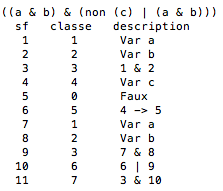
\includegraphics[width=0.3\linewidth]{indexation} %Quelques_formules.f12
\caption{Indexation de la formule $(a\land b)\land(\lnot c \lor (a\land b))$}
\label{fig:indexation}
\end{figure}

%\subsection{Absence de duplication}
%
%
%\
%
%\
%\subsection{Inversibilit� de certaines pr�misses de $\to L$ et $\to R$}
%
%
%$((\bigwedge_{i=1}^{n}p_{i} \lor (\lnot\lnot p_{1}\to f) \lor \bigvee_{i=2}^{n}(p_{i}\to f))\to f)\to f$
%
%\
%
%$(\;[ \;(p_{1}\land p_{2} \land ... \land p_{n}) \lor (\lnot\lnot p_{1}\to f) \lor (p_{2}\to f) \lor ... \lor (p_{n}\to f)\;]\to f\;)\to f$
%
%\
%
%$1:f \quad\To_{0}\quad 0:  p1 \land ( p2 \land p3 )  \;,\; 0: \lnot\lnot p1 \to f  \;,\;  0: p2 \to f  \;,\;  0: p3 \to f  \;,\; 0: f$
%
%\
%
%$f\;;\;\emptyset \quad\To\quad p_{1} \land p_{2} \land ... \land p_{n} \;,\; \lnot\lnot p_{1}\to f \;,\; p_{2}\to f \;,\; ...  \;,\; p_{n}\to f \;,\; f$
%
%
%
%\section{Quelques explications sur l'impl�mentation}
%
%\subsection{Pr�calculs : indexation, classes, priorit�s}
%
%\subsection{Gestion efficace des formules du s�quent : insertion et suppression, choix de la formule principale}
%
%
%
%\section{Vers une recherche de preuve compil�e et certifi�e}
%
%\subsection{Un langage simple pour la certification}
%
%\subsection{Compilation : des fonctions pour chaque sous-formule}
%
%











\section{Impl�mentation}
\subsection{Indexation}

cf ``Propri�t� de la sous-formule et indexation'' + explication sur les classes (et priorit�s) et les champs axiomes du s�quent



\subsection{Structure de donn�es pour le s�quent}




Comme toutes les r�gles de \LSJn\ sont locales, on peut n'avoir � tout moment qu'un seul s�quent en m�moire. Un s�quent de \LSJn\ consiste en deux multiensembles $\G$ et $\D$ de couples ``\emph{ indice\!:\,formule }'' et %un entier $n$ : l'\emph{indice} du s�quent. L'indice 
un \emph{indice} du s�quent $n$. Les indices sont des entiers, et gr�ce � l'indexation, les formules sont aussi des entiers. La question qui se pose est le choix de structure de donn�es pour $\G$ et $\D$.

Consid�rons une des r�gles les plus simples : \LSJLetL. Au cours de l'algorithme de recherche de preuve, on peut �tre amen� � vouloir transformer notre s�quent courant, alors �gal � la conclusion, en la pr�misse. On veut pour cela retirer $i:A\land B$ de $\G$ et y ajouter $i:A$ et $i:B$. On peut aussi avoir besoin de faire la transformations inverse, c'est-�-dire retirer les deux derniers couples et rajouter le premier. Un des objectifs est donc que ces op�rations soient rapides.



On d�finit la complexit� d'une �tape comme la somme des complexit�s dans le pire cas de l'ajout d'un couple, du retrait d'un couple, et du choix d'un couple principal.
%
De simples listes entra�nent bien s�r une complexit� de l'ordre du cardinal des multiensembles. On peut obtenir un choix de couple principal en temps constant avec des listes tri�es, et


\


Au cours de l'algorithme, on manipule un ``s�quent'', cens� repr�senter un s�quent du calcul \LSJn, contenant les informations suivantes :

\noindent-\;
des informations de taille constante : l'indice $n$ du s�quent, et des bool�ens $id$ et $fauxL$, indiquant si les axiomes de m�me nom sont applicables au s�quent ;

\noindent-\;
les couples \emph{indice}: \emph{formule} contenus dans les champs $\G$ et $\D$ du s�quent.

Comme nous l'avons expliqu� en introduisant le calcul \LSJn, le but de celui-ci est de pouvoir effectuer la recherche de preuve en ne gardant � chaque instant qu'un seul s�quent en m�moire.

\


Int�ressons-nous maintenant � la complexit� temporelle.

Celle-ci d�pend du nombre de r�gles qu'on essaie d'appliquer, c'est-�-dire le nombre d'appels r�cursifs � la fonction \emph{prouvable} (?) dont le pseudo-code est donn� en figure ? page ?. Ce nombre d�pend de la taille de la formule et des connecteurs pr�sents dedans (et selon l'ordre dans lequel on choisit les formules principales cela peut beaucoup varier pour une m�me formule, mais on s'int�resse � la complexit� dans le pire cas). Mais il ne d�pend pas de notre choix d'impl�mentation (sauf pour l'ordre des ``implique'', mais encore une fois pas si on regarde le pire cas).










\bibliographystyle{plain}
\bibliography{LSJn}

\end{document}





%%%%%%%%%%%%%%%%%%%%%%%%%%%%%%%
\pagebreak
.
\pagebreak

\section{Le calcul \LSJ}

L'article \cite{LSJ} d�finit un calcul de s�quents \LSJ. Une s�mantique naturelle des s�quents est d�finie � l'aide des mod�les de Kripke, mais nous ne la pr�sentons pas. En effet, ce qui nous int�resse est l'existence, pour toute formule, d'un s�quent qui est prouvable dans le calcul \LSJ\ si, et seulement si, la formule est prouvable en logique intuitionniste. Nous renvoyons � l'article pour les d�monstrations, notamment celle de la compl�tude du calcul.

\subsection{Les s�quents}

On s'int�resse � des \emph{multiensembles}, c'est-�-dire des collections o� le nombre d'occurrences est pris en compte, mais non l'ordre des �l�ments. Cela permettra de ne pas avoir besoin de r�gles explicites d'�change.

Un \textbf{s�quent} est la donn�e de trois multiensembles $\Th$, $\G$ et $\D$ de formules ; on �crit alors $\Th\;;\;\G\;\To\;\D$.

Une d�finition d'un s�quent \textbf{r�futable} est donn�e dans l'article � l'aide des mod�les de Kripke. Nous ne la d�taillons pas ici, car ce qui nous int�resse surtout est la propri�t� suivante qui en d�coule, d�montr�e dans l'article. La d�finition de \textbf{prouvable} sera donn�e plus tard car elle est li�e aux r�gles du calcul, mais ceci illustre son int�r�t.
\begin{prop}\label{propSignificationSequent}
%Soit $\G$, $\D$ des multiensembles de formules. Le s�quent $\emptyset\;;\;\G\;\To\;\D$ est \textbf{prouvable} dans \LSJ, c'est-�-dire non r�futable, si et seulement si la formule $\bigwedge_{A\in\G}A\,\to\,\bigvee_{B\in\D}B$ est valide en logique intuitionniste.
Un s�quent $\emptyset\;;\;\G\;\To\;\D$ est \textbf{r�futable} si, et seulement si, la formule $\bigwedge_{A\in\G}A\,\to\,\bigvee_{B\in\D}B$ n'est pas valide en logique intuitionniste. Un s�quent est \textbf{prouvable} dans \LSJ\ si, et seulement si, il n'est pas r�futable.

\end{prop}
\begin{cor}
Soit $A$ une formule, elle est valide en logique intuitionniste si et seulement si le s�quent $\emptyset;\emptyset\To A$ est  prouvable dans \LSJ.
\end{cor}

Les multiensembles $\G$ et $\D$, et leur signification dans la propri�t� \ref{propSignificationSequent} sont des �l�ments habituels en calcul des s�quents. En revanche, $\Th$ est propre � \LSJ, et est difficile � interpr�ter car contrairement au cas o� $\Th$ est vide, un s�quent avec $\Th$ quelconque ne peut pas �tre repr�sent� par une formule. On peut dire est que $\Th$ contient des formules gard�es en r�serve, non visibles directement dans le s�quent (une formule de $\Th$ ne peut pas �tre \emph{formule principale}), mais qui peuvent �tre transf�r�es dans $\G$ et ainsi devenir visibles. On verra que les seules r�gles qui agissent sur $\Th$ sont celles qui concernent le connecteur $\to$.

Pour un s�quent $\Th\;;\;\G\;\To\;\D$, on appellera les formules de $\G$ les \textbf{formules de gauche}, celles de $\D$ les \textbf{formules de droite}, et celles de $\Th$ les \textbf{formules de r�serve} du s�quent (appellations non conventionnelles).

%

\subsection{Les r�gles}

%Une r�gle est de la forme\regle o� $\mathcal R$ est le nom de la r�gle, et $prem_{1}$, ... , $prem_{p}$, $concl$ d�crivent des s�quents d'une certaine forme. Par exemple $\Th\;;\;A\lor B,\G\;\To\;\D$ repr�sente n'importe quel s�quent o� au moins une des formules de gauche est une disjonction, et si $\Th\;;\;A,\G\;\To\;\D$ se trouve dans la m�me r�gle, cela repr�sente un s�quent obtenu � partir du pr�c�dent en rempla\c cant une disjonction de gauche $A\lor B$ par son premier terme $A$.



Les r�gles du calcul \LSJ\ sont donn�es dans la figure~\ref{fig:reglesLSJ}. La notation $A,\G$ repr�sente le multiensemble obtenu � partir de $\G$ en ajoutant une occurrence de $A$. Pour une r�gle \regle, $\mathcal R$ est le nom de la r�gle, $prem_{1}$, ... , $prem_{p}$ sont les (resp. premi�re, ... , $p$-i�me) \textbf{pr�misses}, et $concl$ la \textbf{conclusion}. Les \textbf{axiomes} sont les r�gles sans pr�misse. Pour toutes les autres r�gles, une unique formule appara�t de mani�re explicite dans la conclusion : c'est la \textbf{formule principale}. Les r�gles dites de gauche, ou d'introduction � gauche, contenant un $L$ dans leur nom, sont celles o� la formule principale se trouve � gauche dans la conclusion, de m�me pour les r�gles de droite.

\begin{figure}
\centering

$$\begin{array}{cc}
	\LSJfauxL & \Id \\\\
	\LSJetL & \LSJetR \\\\
	\LSJouL & \LSJouR \\\\
	\multicolumn{2}{c}{\LSJimpL}\\\\
	\multicolumn{2}{c}{\LSJimpR}
\end{array}$$

\caption{Les r�gles du calcul \LSJ}
\label{fig:reglesLSJ}
\end{figure}


Une \textbf{instance} d'une r�gle $\mathcal R$ a la m�me forme que la r�gle : \instance, mais ici les $\s_{i}$ et $\s$ sont des s�quents connus explicitement ; bien entendu il faut qu'il s'agisse de s�quents qui ont bien la forme donn�e par la d�finition de la r�gle. Par exemple \LSJetL\ devient une instance de la r�gle $\land L$ (qui a la m�me �criture que la r�gle) lorsqu'on conna�t les formules $A$ et $B$ et toutes les formules de $\Th$, $\G$, $\D$.

Une \textbf{preuve} est un arbre dont les n\oe uds sont �tiquet�s par un s�quent et une r�gle et ont la m�me arit� que le nombre de pr�misses de la r�gle, et tel que : pour tout n\oe ud de s�quent $\s$ et r�gle $\mathcal R$, si $\s_{1}$, ... , $\s_{p}$ sont les s�quents associ�s � chacun de ses fils respectivement, alors \instance\ est une instance de $\mathcal R$. Les feuilles d'un tel arbre sont les n\oe uds auxquels est associ� un axiome.

Un s�quent est \textbf{prouvable} s'il existe une preuve � la racine de laquelle il est associ�.

De mani�re �quivalente, on peut d�finir l'ensemble des formules prouvables comme le plus petit ensemble v�rifiant : pour toute instance \instance\ d'une r�gle de \LSJ, si pour tout $i$, $\s_{i}$ est prouvable, alors $\s$ est prouvable (en particulier pour toute instance \instanceAx\ d'un axiome $\mathcal A$, $\s$ est prouvable).



\subsection{Conditions de non-prouvabilit�}

Pour montrer qu'un s�quent est prouvable, il suffit d'en exhiber une preuve. Comment montrer le contraire ? D'apr�s la d�finition pr�c�dente, un s�quent n'est pas prouvable s'il n'existe aucune instance de r�gle\instance telle que tous les $\s_{i}$ sont prouvables. Or les $\s_{i}$ ne d�pendent que de $\s$, $\mathcal R$ et du choix de la formule principale : il est donc possible de tester toutes les instances possibles. Cela fournit un premier algorithme de recherche de preuve : r�cursivement, pour chercher si un s�quent $\s$ est prouvable, on consid�re toutes les instances de r�gles dont $\s$ est la conclusion et pour chacune on d�termine r�cursivement si chaque pr�misse est prouvable. Si on trouve une instance telle que toutes les pr�misses sont prouvables, alors $\s$ est prouvable (et on obtient une preuve de $\s$ si on conna�t une preuve de chacune de ces pr�misses), sinon $\s$ n'est pas prouvable. Cet algorithme est tr�s long. En fait, c'est � peu pr�s ce qu'on se retrouve � faire dans les cas extr�mement d�favorables. Mais heureusement, on a un proc�d� bien plus �conome en moyenne gr�ce � la notion de r�gle ou pr�misse inversible.

Une pr�misse $prem_{i}$ d'une r�gle\regle(aussi appel�e $i$-�me pr�misse de $\mathcal R$) est \textbf{inversible} si on a : si $prem_{i}$ est non prouvable, alors $concl$ est non prouvable. Une r�gle est \textbf{inversible} si toutes ses pr�misses sont inversibles.

On admet, une d�monstration se trouvant dans l'article \cite{LSJ} :

\noindent- les r�gles $\land L$, $\land R$, $\lor L$ et $\lor R$ sont inversibles~;

\noindent- les deux premi�res pr�misses de $\to L$ et la premi�re pr�misse de $\to R$ sont inversibles~;

\noindent- la troisi�me pr�misse de $\to L$ et la deuxi�me pr�misse de $\to R$ ne sont pas inversibles.



\subsection{Algorithme}


On en d�duit le proc�d� suivant pour essayer d'appliquer une r�gle � un s�quent avec un formule principale donn�e : on essaie de prouver les pr�misses inversibles, puis l'�ventuelle pr�misse non inversible (dans \LSJ\ il y en a au plus une). D�s qu'on trouve qu'une pr�misse inversible est non prouvable, on s'arr�te : le s�quent initial n'est pas prouvable non plus. Si toutes les pr�misses sont prouvables, le s�quent initial est �galement prouvable. Dans le dernier cas (seule la pr�misse non inversible est non prouvable), on essaie une application de r�gle avec une autre formule principale.

Il ne reste plus qu'� d�cider dans quel ordre les formules qui peuvent l'�tre sont choisies comme formule principale pour essayer d'appliquer une r�gle. On choisit de traiter en premier les r�gles inversibles, car on sait alors qu'il n'y aura pas besoin d'essayer d'autre application de r�gle sur le m�me s�quent. 
% : apr�s avoir examin� au pire toutes les pr�misses, on sait si le s�quent est prouvable.
Parmi celles-ci, on privil�gie celles qui n'ont qu'une pr�misse ($\land L$ et $\lor R$) sur les autres, qui en ont deux ($\lor L$ et $\land R$).

%L'algorithme est le suivant.

\begin{figure}[!h]
%\centering
\def\true{\emph{vrai}}
\def\false{\emph{faux}}
\def\lett{\textbf{soit }}
\def\if{\textbf{si} }
\def\then{\textbf{alors} }
\def\return{\textbf{retourner} }
\def\select{\textbf{s�lectionner} }
\def\from{\textbf{dans} }

\textbf{fonction} estProuvable ($\s$)

\quad \lett $\s=\Th;\G\To\D$

\quad \if ($\bot\in\G$) \then \return \true

\quad \if ($\G\cap\D\neq\emptyset$) \then \return \true

\quad \if ($\G$ et $\D$ ne contiennent que des formules \emph{atomiques}) \then \return \false


\quad \if (il existe $A\land B\in\G$) \then $\{$

\quad \quad \select $H=A\land B$ \from $\G$

\quad \quad \return estProuvable($prem(\land L, \s, H)$)

\quad $\}$


\quad \if (il existe $A\lor B\in\D$) \then $\{$

\quad \quad \select $H=A\lor B$ \from $\D$

\quad \quad \return estProuvable($prem(\lor R, \s, H)$)

\quad $\}$

\quad ...


\caption{Algorithme}
\label{fig:algo}
\end{figure}



\subsection{?}




On voit imm�diatement que l'algorithme n�cessite de pouvoir d�duire d'un s�quent, d'une r�gle et d'une formule principale contenue dans le s�quent et sur laquelle la r�gle peut agir, les s�quents correspondant aux diff�rentes pr�misses. Ce n'est pas difficile : pour les axiomes il n'y a rien � faire ; pour les autres r�gles, la formule principale $H$ �tant de la forme $A \text{ 'connecteur' } B$, il suffit d'enlever $H$ du s�quent et, selon le connecteur et le c�t� o� se trouvait $H$, d'ajouter $A$ ou $B$ � $\Th$, $\G$, $\D$ ou nulle part.

Mais ce n'est pas tout. Lorsqu'on essaie d'appliquer une r�gle\instancedeux\ au s�quent $\s$, on lance une recherche de preuve sur $\s_{1}$ qu'on a obtenu comme d�crit ci-dessus. Si on obtient que $\s_{1}$ est prouvable, on lance alors la recherche de preuve sur $\s_{2}$. On doit donc d�terminer $\s_{2}$. On a vu qu'on sait le faire � partir de $\s$. Une solution consiste donc � retenir $\s$ pendant qu'on effectue la recherche de preuve sur $\s_{1}$, mais cela peut �tre co�teux en m�moire. Une autre solution, que nous avons privil�gi�e, consiste � �tre capable de retrouver $\s$ � partir de $\s_{1}$ ainsi que de la formule principale, de la r�gle et du num�ro de la pr�misse (ici $1$). On a dans ce cas besoin de pouvoir retrouver la conclusion � partir de n'importe laquelle des pr�misses, pas seulement par exemple de la premi�re pr�misse pour une r�gle qui n'en a que deux. En effet, utiliser $\s_{1}$ pour retrouver $\s$ suppose qu'� la fin de la recherche de preuve pour $\s_{1}$, on conna�t $\s_{1}$. Or, l'id�e ici est de n'avoir vraiment qu'un seul s�quent en m�moire � tout moment. Ainsi, � la fin de la recherche de preuve pour $\s$, on doit conna�tre $\s$, donc on doit aussi pouvoir d�duire $\s$ de $\s_{2}$ en connaissant la formule principale et le fait qu'on est en train de s'int�resser � la deuxi�me pr�misse.

En r�sum�, on aimerait (bien que ce ne soit pas n�cessaire) que toutes les r�gles soient \textbf{locales}, avec la d�finition suivante.

\begin{df}
Une r�gle est \textbf{locale} si pour toute instance\instance\ de cette r�gle et pour tout $i$ entre $1$ et $p$, on peut d�duire $\s$ � partir de $\s_{i}$ et de la formule principale et de $i$.
\end{df}

On remarque que $\land L$, $\land R$, $\lor L$ et $\lor R$ sont locales. Les axiomes sont �galement locaux, la d�finition n'ayant pas grand int�r�t pour eux. En revanche, les r�gles $\to L$ et $\to R$ ne sont pas locales : pour chacune, les formules repr�sent�es par $\D$ dans la conclusion n'apparaissent nulle part dans la derni�re pr�misse, il n'est donc pas possible de retrouver la conclusion en connaissant uniquement cette pr�misse, la formule principale et le num�ro de la pr�misse, puisqu'il n'y a aucun moyen d'en d�duire ce qui se trouve dans $\D$.

C'est pour cette raison qu'on introduit le calcul \LSJn, dans lequel toutes les r�gles sont locales.

\section{Le calcul \LSJn}


%On utilise les d�finitions et notations de l'article~\cite{LSJ}.
%.
%
%\
%
%Le syst�me \LSJn\ a pour objectif de faire les m�mes calculs que \LSJ, mais en manipulant des s�quents qui contiennent un peu plus d'information, afin de pouvoir faire le ``back-tracking'' n�cessaire � l'algorithme de \LSJ\ en n'ayant � tout moment en m�moire qu'un seul s�quent.
%
%Pour cela, on veut que les s�quents de \LSJn\ repr�sentent de mani�re exhaustive et pertinente ceux de \LSJ\ : on montre qu'il existe une surjection de l'ensemble des s�quents de \LSJn\ dans l'ensemble des s�quents de \LSJ, telle qu'un s�quent de \LSJn\ est prouvable dans \LSJn\ si, et seulement si, son image est prouvable dans \LSJ.
%
%\
%
%Le calcul \LSJn, tr�s proche du calcul \LSJ, manipule des s�quents contenant un peu plus d'information afin de n'avoir que des r�gles locales. 
%Plus pr�cis�ment, chaque s�quent de \LSJn\ a un indice (un entier naturel), et chaque formule du s�quent a �galement un indice.
%Plus pr�cis�ment, chaque s�quent a un indice $n$, qui d�termine lesquelles de ses formules, qui ont aussi chacune un indice $i$, sont \emph{actives}, c'est-�-dire peuvent �tre la formule principale lors d'une application de r�gle : pour les formules de gauche, la condition est $i\leq n$, et pour celles de droite $i=n$. Ainsi, pour la derni�re pr�misse des deux r�gles li�es � $\to$ par exemple, les formules de droite de la conclusion peuvent �tre conserv�e dans le s�quent sans �tre actives. Il suffit de modifier l'indice du s�quent pour changer les formules actives.

Le calcul \LSJn\ est tr�s proche du calcul \LSJ\ : chaque r�gle de \LSJn\ correspond � une r�gle de \LSJ, et des arbres de preuve dans les deux syst�mes pour la m�me formule sont fortement li�s. Mais contrairement � \LSJ, les r�gles de \LSJn\ sont toutes locales. Pour cela, les s�quents de \LSJn\ repr�sentent chacun un s�quent de \LSJ, avec un peu plus d'informations : celles qui sont parfois n�cessaire pour retrouver la conclusion � partir d'une pr�misse. Cette repr�sentation est exhaustive et correcte. On montre en effet qu'il existe une surjection de l'ensemble des s�quents de \LSJn\ dans l'ensemble des s�quents de \LSJ, telle qu'un s�quent de \LSJn\ est prouvable dans \LSJn\ si, et seulement si, son image est prouvable dans \LSJ.


\subsection{Formalisme de \LSJn}


Un s�quent de \LSJn\ est la donn�e de deux multiensembles $\Gp$ et $\Dp$ de couples $entier~:~formule$, et d'un entier naturel $n$, tels que tous les entiers pr�sents dans $\Gp$ sont $\leq n+1$ et tous ceux pr�sents dans $\Dp$ sont $\leq n$ ; on �crit $\Gp \Rightarrow_{n} \Dp$.

\

Les r�gles du calcul \LSJn\ sont d�crite dans la figure~\ref{fig:reglesLSJn}. Chacune correspond � une r�gle de \LSJ.


\begin{figure}[h]
\centering

\emph{$n$ et parfois $i$ d�signent toujours des entiers naturels, avec $i\leq n$}
$$\begin{array}{cc}
	\LSJLfauxL & \Id \\\\
	\LSJLetL & \LSJLetR \\\\
	\LSJLouL & \LSJLouR \\\\
	\multicolumn{2}{c}{\LSJLimpL}\\\\
	\multicolumn{2}{c}{\LSJLimpR}
\end{array}$$

\caption{Les r�gles du calcul \LSJn}
\label{fig:reglesLSJn}
\end{figure}




\subsection{\'Equivalence avec \LSJ}


On note $\Sig$ l'ensemble des s�quents de \LSJ, et $\Sig'$ l'ensemble des s�quents de \LSJn.

Soit $\sigma\in\Sig$, on note $\vdash\sigma$ si $\sigma$ est prouvable dans \LSJ\ ; soit $\sigma'\in\Sig'$, on note $\vdash'\sigma'$ si $\sigma'$ est prouvable dans \LSJn.

\

Soit $M$ un multiensemble de couples $entier:formule$, l'entier d'un couple �tant appel� son indice. On note $M_{k}$ le multiensemble obtenu � partir de $M$ en ne gardant que les couples d'indice $k$, et $M_{\leq k}$ celui obtenu en ne gardant que les couples d'indice inf�rieur � $k$. On note $\forget(M)$ le multiensemble de formules obtenu en oubliant l'indice et ne gardant que la formule de chaque couple de $M$.

On d�finit l'application $\surj$ de %l'ensemble des s�quents de \LSJn\ dans l'ensemble des s�quents de \LSJ,
$\Sig'$ dans $\Sig$, qui � $\G' \To_{n} \D'$ associe $\Th\, ;\G \To \D$ %\quad 

\noindent
o� :\;
$\left\{
\begin{array}{l}
%	\Th = \{ A \:|\: n+1:A \in \G'\} \\
%	\G = \{ A \:|\: \exists i\leq n,\ i:A \in \G'\} \\
%	\D = \{ A \:|\: n:A \in \D'\}
	\Th = \forget (\G'_{n+1}) \\
	\G = \forget (\G'_{\leq n}) \\
	\D = \forget (\D'_{n})
\end{array}
\right.$.

C'est une application surjective : en effet tout s�quent $\Th \,;\G\To\D$ de \LSJ\ a au moins pour ant�c�dent le s�quent $\G' \To_{0} \D'$, 
%avec $\G' = \{ 0:A \:|\: A \in \G\} \cup \{ 1:A \:|\: A \in \Th\}$ et $\D' = \{ 0:A \:|\: A \in \D\}$.
o� $\G'$ est l'union de $0 : \G$ (le multiensemble de couples obtenu � partir de $\G$ en rempla\c cant chaque occurrence d'une formule $A$ par une occurrence du couple $0:A$) avec $1:\Th$, et o� $\D'=0:\D$.

\




Soit $\mathcal R$ une r�gle de \LSJ. On note $\mathcal R'$ la r�gle de \LSJn\ qui lui correspond. On �crit \instanceR\ et \instanceRp\ des instances de ces r�gles.


\begin{lm}
Soit $\sigma\in\Sig$ et $\sigma'\in\Sig'$ tels que $\sigma=\surj(\sigma')$ et soit $\mathcal R$ une r�gle de \LSJ.

1) Si \instanceR alors il existe $\s'_{1}$, ... , $\s'_{p}$ tels que pour tout $k$, $\s_{k} = \surj (\s'_{k})$, et \instanceRp.

2) Si \instanceRp, posons pour tout $k$, $\s_{k} = \surj (\s'_{k})$, alors \instanceR.

\noindent
Pour un axiome $\mathcal A$, cela signifie simplement : \instanceAx si et seulement si \instanceAxp.
\end{lm}

\begin{proof}
On le montre pour chaque r�gle ; c'est une cons�quence assez directe de la d�finition de $\surj$. Faisons-le par exemple pour Id, $\land R$ et $\to L$. \`A chaque fois, on se donne $\s = \Th\, ;\G \To \D$ et $\s' = \G' \To_{n} \D' \in\Sig'$ tels que $\s=\surj(\s')$.

\

%\noindent-\quad 
\noindent Id :\quad On a\instanceId\ si et seulement s'il existe une formule $A$ appartenant � la fois � $\G$ et $\D$, ce qui �quivaut, par d�finition de $\surj$, � : il existe $A$ et $i\leq n$ tels que $n:A\in\D'$ et $i:A\in\G'$, c'est-�-dire \instanceIdp.

\

\noindent $\land R$ :	\quad

1) Si \instanceetR\ alors il existe des formules $A$ et $B$ et un multiensemble $\Dt$ tels que $\D = A \land B, \Dt$ et $\s_{1} = \Th\, ;\G \To A,\Dt$ et $\s_{2} = \Th\, ;\G \To B,\Dt$.
 Posons $\Dt' = \D' - n:A \land B$ le multiensemble obtenu en retirant une seule occurrence de $n:A\land B$ � $\D'$ (qui contient cet �l�ment parce que $\D$ contient $A\land B$ et par d�finition de $\surj$),
 et $\s'_{1} = \G' \To_{n} n:A,\Dt'$ et $\s'_{2} = \G' \To_{n} n:B,\Dt'$.
 Alors on a bien $\s_{1}=\surj(\s'_{1})$ et $\s_{2}=\surj(\s'_{2})$ (en remarquant que 
 %$\Dt = \{ C \:|\: n:C \in \Dt'\}$
$\Dt = \forget (\Dt'_{n})$
), et \instanceetRp (en remarquant que $\s' = \G' \To_{n} n:A \land B,\Dt'$).

2) Si \instanceetRp\ alors il existe $A$, $B$ et $\Dt'$ tels que $\D' = n:A \land B, \Dt'$ et $\s'_{1} = \G' \To_{n} n:A,\Dt'$ et $\s'_{2} = \G' \To_{n} n:B,\Dt'$ ; 
 on pose $\Dt = \D - A \land B$ le multiensemble obtenu en retirant une seule occurrence de $A\land B$ � $\D$,
 et $\s_{1}=\surj(\s'_{1})$ et $\s_{2}=\surj(\s'_{2})$ ; on obtient $\s = \Th\, ;\G \To A\land B,\Dt$ et $\s_{1} = \Th\, ;\G \To A,\Dt$ et $\s_{2} = \Th\, ;\G \To B,\Dt$\; d'o�\instanceetR.

\

\noindent $\to L$ :	\quad

1) Si \instanceimpL\ alors il existe $A$, $B$ et $\Gt$ tels que $\G=A\to B,\Gt$ et $\s_{1} = \Th\, ;B,\Gt \To \D$ et $\s_{2} = B,\Th\, ;\Gt \To A,\D$ et $\s_{3} = B \,; \Th,\Gt \To A$ ; et il existe $i\leq n$ tel que $i:A\to B\in\G'$ ;
 on pose $\Gt' = \G' - i:A\to B$ (on retire une seule occurrence de $i:A\to B$ de $\G'$) et $\s'_{1} = i:B,\Gt' \To_{n} \D'$ et $\s'_{2} = n+1:B,\Gt' \To_{n} n:A,\D'$ et $\s'_{3} = n+2:B,\Gt' \To_{n+1} n+1:A, \D'$ et on v�rifie que cela convient.

2) Si \instanceimpLp\ alors il existe $i$, $A$, $B$ et $\Gt'$ tels que $\G'=i:A\to B,\Gt'$ et $\s'_{1}$, $\s'_{2}$ et $\s'_{3}$ ont la forme donn�e ci-dessus ; on pose $\Gt = \G - A\to B$ (on retire une seule occurrence de $A\to B$ de $\G$), alors les images $\s_{1}$, $\s_{2}$ et $\s_{3}$ par $\surj$ de $\s'_{1}$, $\s'_{2}$ et $\s'_{3}$ respectivement s'�crivent comme ci-dessus et donc \instanceimpL.
\end{proof}



\begin{theo}
Soit $\sigma\in\Sig$ et $\sigma'\in\Sig'$ tels que $\sigma=\surj(\sigma')$, alors $\vdash \sigma$ si et seulement si $\vdash' \sigma'$.
%Soit $\sigma$ un s�quent de \LSJ\ et $\sigma'$ un s�quent de \LSJn\ tels que $\sigma=\surj(\sigma')$, alors $\vdash \sigma$ si et seulement si $\vdash' \sigma'$.
\end{theo}

\begin{proof}
Par r�currence sur la \emph{taille} de $\s\in\Sig$, c'est-�-dire la somme des tailles des formules des trois multiensembles apparaissant dans $\s$.

\

\noindent
On initialise pour tout $\sigma = \Th\, ;\G \To \D$ tel que toutes les formules dans $\G$ et dans $\D$ sont atomiques : soit $\sigma' = \G' \To_{n} \D' \in\Sig'$ tel que $\sigma=\surj(\sigma')$. Alors toutes les formules associ�es � un $i \leq n$ dans $\G'$ et toutes les formules associ�es � $n$ dans $\D'$ sont aussi atomiques. En �tudiant la forme des conclusions des r�gles non axiomatiques de \LSJ\ comme de \LSJn,
on remarque que si $\s$ (resp. $\s'$) est la conclusion d'une r�gle de \LSJ\ (resp. \LSJn), alors la r�gle est un axiome. L'initialisation est donc un cas particulier de ce qui suit avec $p=0$ (ce qui entra�ne qu'on n'utilise en fait pas l'hypoth�se de r�currence).

% on obtient que : $\vdash \s$ si et seulement si $\s$ est une cons�quence directe d'un axiome de \LSJ, et $\vdash' \s'$ si et seulement si $\s'$ est une cons�quence directe d'un axiome de \LSJn. Or d'apr�s le lemme, pour $\mathcal A$ axiome de \LSJ, \instanceAx si et seulement si \instanceAxp. On en d�duit $\vdash \sigma$ si et seulement si $\vdash' \sigma'$.

\

\noindent
Soit $\s = \Th\, ;\G \To \D \in\Sig$. Soit $\sigma' = \G' \To_{n} \D' \in\Sig'$ tel que $\sigma=\surj(\sigma')$.

On suppose $\vdash \s$. Alors il existe une r�gle $\mathcal R$ de \LSJ\ et $\s_{1}$, ... , $\s_{p} \in\Sig$ (avec �ventuellement $p$ nul) tels que $\vdash \s_{k}$ pour tout $k$ et\instanceR. D'apr�s le lemme, il existe $\s'_{1}$, ... , $\s'_{p} \in\Sig'$ tels que $\s_{k}=\surj(\s'_{k})$ pour tout $k$ et\instanceRp. Pour tout $k$, on applique l'hypoth�se de r�currence � $\s_{k}$ qui a une \emph{taille} strictement inf�rieure � celle de $\s$, et on obtient $\vdash' \s'_{k}$. On en d�duit $\vdash' \s'$.

On suppose $\vdash' \s'$. Alors il existe une r�gle $\mathcal R'$ de \LSJn\ et $\s'_{1}$, ... , $\s'_{p} \in\Sig'$ tels que $\vdash' \s'_{k}$ pour tout $k$ et\instanceRp. On pose $\s_{k}=\surj(\s'_{k})$ pour tout $k$. D'apr�s le lemme on a \instanceR, en particulier on peut appliquer l'hypoth�se de r�currence aux $\s_{k}$ donc $\vdash \s_{k}$ pour tout $k$, d'o� $\vdash \s$.

\end{proof}






\section{Efficacit� de \LSJ}


L'�tude qui suit porte sur le calcul \LSJ. En effet, \LSJn\ h�rite de toutes les propri�t�s int�ressantes de \LSJ, en apportant une localit� des r�gles qui facilite une impl�mentation �conome en m�moire.


\subsection{Propri�t� de la sous-formule et indexation}

$B$ est une \textbf{sous-formule} de $A$ si $B=A$ ou si $A$ est de la forme $A_{1}$`connecteur'$A_{2}$ et ($B$ est une sous-formule de $A_{1}$ ou $B$ est une sous-formules de $A_{2}$). Un calcul de s�quents v�rifie la \textbf{propri�t� de la sous-formule} si tout s�quent prouvable $\s$ admet une preuve telle que toute formule apparaissant dans (un s�quent de) la preuve est une sous-formule d'une formule de $\s$. En particulier, le s�quent $\To A$ a une preuve dans laquelle toute formule est une sous-formule de $A$.

Le calcul \LSJ v�rifie la propri�t� de la sous-formule : on le constate ais�ment en observant chaque r�gle.

La propri�t� de la sous-formule est tr�s recherch�e en calcul des s�quents. D'une part, elle donne une borne sur les formules qu'il faudra manipuler au cours d'une recherche de preuve, qui sont �videmment toutes plus petites que la formule qu'on essaie de prouver. Mais surtout, elle permet de conna�tre � l'avance la liste exhaustive des formules qu'on pourra rencontrer. On peut donc � l'avance les num�roter : ainsi, les formules d'un s�quents sont simplement repr�sent�es par un entier. Il faut quelques informations sur ces num�ros : par exemple pour une formule $A\land B$, il faut savoir qu'il s'agit d'un ``et'', et pouvoir d�terminer $A$ et $B$. Il faut aussi pouvoir reconna�tre quand l'axiome Id (une m�me formule appara�t des deux c�t�s du s�quent) s'applique : pour cela on associe � chaque formule une classe, qui correspond � une classe d'�quivalence de la relation d'�galit� structurelle. La taille de toutes ces informations r�unies est lin�aire en la taille de la formule de d�part (c'est-�-dire le nombre de n\oe uds de l'arbre qui la repr�sente, qui est aussi le nombre de sous-formules avec multiplicit�). Un exemple est donn� par la figure~\ref{fig:indexation}.

La propri�t� de la sous-formule est encore plus int�ressante dans le cadre de la recherche de preuve compil�e : conna�tre � l'avance les formules qui appara�tront permet d'�crire pour chacune des fonctions agissant sur le s�quent, au lieu de les calculer au cours de la recherche de preuve (voir ??).

\begin{figure}
%\centering
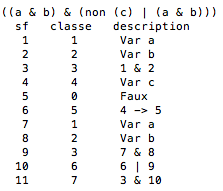
\includegraphics[width=0.3\linewidth]{indexation} %Quelques_formules.f12
\caption{Indexation de la formule $(a\land b)\land(\lnot c \lor (a\land b))$}
\label{fig:indexation}
\end{figure}

%\subsection{Absence de duplication}
%
%
%\
%
%\
%\subsection{Inversibilit� de certaines pr�misses de $\to L$ et $\to R$}
%
%
%$((\bigwedge_{i=1}^{n}p_{i} \lor (\lnot\lnot p_{1}\to f) \lor \bigvee_{i=2}^{n}(p_{i}\to f))\to f)\to f$
%
%\
%
%$(\;[ \;(p_{1}\land p_{2} \land ... \land p_{n}) \lor (\lnot\lnot p_{1}\to f) \lor (p_{2}\to f) \lor ... \lor (p_{n}\to f)\;]\to f\;)\to f$
%
%\
%
%$1:f \quad\To_{0}\quad 0:  p1 \land ( p2 \land p3 )  \;,\; 0: \lnot\lnot p1 \to f  \;,\;  0: p2 \to f  \;,\;  0: p3 \to f  \;,\; 0: f$
%
%\
%
%$f\;;\;\emptyset \quad\To\quad p_{1} \land p_{2} \land ... \land p_{n} \;,\; \lnot\lnot p_{1}\to f \;,\; p_{2}\to f \;,\; ...  \;,\; p_{n}\to f \;,\; f$
%
%
%
%\section{Quelques explications sur l'impl�mentation}
%
%\subsection{Pr�calculs : indexation, classes, priorit�s}
%
%\subsection{Gestion efficace des formules du s�quent : insertion et suppression, choix de la formule principale}
%
%
%
%\section{Vers une recherche de preuve compil�e et certifi�e}
%
%\subsection{Un langage simple pour la certification}
%
%\subsection{Compilation : des fonctions pour chaque sous-formule}
%
%











\section{Impl�mentation}
\subsection{Indexation}

cf ``Propri�t� de la sous-formule et indexation'' + explication sur les classes (et priorit�s) et les champs axiomes du s�quent



\subsection{Structure de donn�es pour le s�quent}

Au cours de l'algorithme, on manipule un ``s�quent'', cens� repr�senter un s�quent du calcul \LSJn, contenant les informations suivantes :

\noindent-\;
des informations de taille constante : l'indice $n$ du s�quent, et des bool�ens $id$ et $fauxL$, indiquant si les axiomes de m�me nom sont applicables au s�quent ;

\noindent-\;
les couples \emph{indice}: \emph{formule} contenus dans les champs $\G$ et $\D$ du s�quent.

Comme nous l'avons expliqu� en introduisant le calcul \LSJn, le but de celui-ci est de pouvoir effectuer la recherche de preuve en ne gardant � chaque instant qu'un seul s�quent en m�moire.

\


Int�ressons-nous maintenant � la complexit� temporelle.

Celle-ci d�pend du nombre de r�gles qu'on essaie d'appliquer, c'est-�-dire le nombre d'appels r�cursifs � la fonction \emph{prouvable} (?) dont le pseudo-code est donn� en figure ? page ?. Ce nombre d�pend de la taille de la formule et des connecteurs pr�sents dedans (et selon l'ordre dans lequel on choisit les formules principales cela peut beaucoup varier pour une m�me formule, mais on s'int�resse � la complexit� dans le pire cas). Mais il ne d�pend pas de notre choix d'impl�mentation (sauf pour l'ordre des ``implique'', mais encore une fois pas si on regarde le pire cas).










\bibliographystyle{plain}
\bibliography{LSJn}

\end{document}















\bibliographystyle{plain}
\bibliography{memoire_stage}


\end{document}
